%*********************************************************************
% gdutthesis: 广东工业大学论文模板
% 2021/11/09 v0.1c
%
% 重要提示:
%   1. 请确保使用 UTF-8 编码保存
%   2. 请使用 XeLaTeX 或 LuaLaTeX 编译
%   3. 请仔细阅读用户文档和 Wiki
%   4. 修改、使用、发布本文档请务必遵循 LaTeX Project Public License
%   5. 不需要的注释可以尽情删除
%*********************************************************************
\let\cleardoublepage\clearpage
\documentclass[
  % type=doctor
  type=master
  % type=promaster
]{gdutthesis}

% 宏包在这里加载
\usepackage{siunitx}[=v2]
\usepackage{zhlipsum,lipsum}
\usepackage{algorithm}
\usepackage{algorithmic}
%\usepackage[gbpub=false]{biblatex}

\gdutsetup{
  style = {
    cover           = {true},
    % cover           = {false},
    % font            = {garamond},
    % font            = {libertinus},
    % font            = {lm},
    % font            = {palatino},
    font            = {times},
    % font            = {times*},
    cjk-font        = {fandol},
    % cjk-font        = {founder},
    % cjk-font        = {mac},
    % cjk-font        = {sourcehan},
    % cjk-font        = {noto},
    % cjk-font        = {windows},
    % cjk-font        = {none},
%    bib-backend     = {bibtex},
     bib-backend     = {biblatex},
    bib-resource    = {gdutthesis-template.bib},
    bib-style       = {numerical},
    % bib-style       = {author-year},
%    fullwidth-stop  = {mapping},
    % fullwidth-stop  = {catcode},
     fullwidth-stop  = {false},
%    hyperlink       = {color},
    % hyperlink       = {border},
     hyperlink       = {none},
    hyperlink-color = {default},
    % hyperlink-color = {autumn},
    % hyperlink-color = {business},
    % hyperlink-color = {classic},
    % hyperlink-color = {elegant},
    % hyperlink-color = {fantasy},
    % hyperlink-color = {material},
    % hyperlink-color = {science},
    % hyperlink-color = {summer},
    % hyperlink-color = {graylevel},
    % hyperlink-color = {prl},
  },
  info = {
    title           = {基于多源信息融合的多旋翼飞行器状态估计方法研究},
    title*          = {Research on state estimation method of multi-rotor aircraft based on multi-source information fusion},
    date            = {2022/5/23},
    author          = {邓正雄},
    author*         = {Deng Zhengxiong},
    supervisor      = {鲁仁全\qquad 教授},
%    supervisor      = {鲁仁全},
    supervisor*     = {Prof. Lu Renquan},
%    author          = {2111904069},
%    author*         = {2111904069},
%    supervisor      = {***},
%    supervisor*     = {***},
    supervisor-two  = {none},
    supervisor-two* = {none},
    department      = {自动化学院},
    department*     = {Automation},
    major           = {控制科学与工程},
    student-id      = {2111904069},
    chairman        = {裴海龙\qquad 教授},
%    chairman        = {***},
    degree          = {工学硕士},
    degree*         = {(Master of Engineering Science)},
    keywords        = {多旋翼, IMU校准, 状态估计, 多传感器融合},
    keywords*       = {Multi-rotor, IMU calibration, State estimation, Multi-sensor fusion},
    secret-level    = {none},
  }
}


\begin{document}

\begin{abstract}
	多旋翼飞行器由于具有体积小、机动性好和悬停能力强的特点,是执行室内外多场景作业的理想平台。
	随着近年来飞行器技术的快速发展,多旋翼飞行器已经广泛应用于各种场景当中。
	对于多旋翼飞行器,其关键技术是飞控系统中的状态估计以及运动控制。
	本文针对恶劣环境下多旋翼飞行器状态估计的安全性要求,提出了以下两个关键技术问题:
	1)如何校准低成本传感器的误差参数从而获得精确可靠的测量值;
	2)如何融合多源信息以提高飞行器状态估计的准确性和鲁棒性。
	因此,本文针对具有重要工程价值的上述关键技术问题设计了包括传感器校准算法、状态估计算法以及控制算法在内的解决方案。
	本研究的具体内容及成果如下:
	
	(1) 针对如何校准低成本传感器误差参数的问题,首先针对IMU的误差,给出了传感器误差模型,分析了各种校准算法的优劣性,并通过实验分析指出,基于残差和分割阈值的校准方法在样本数较少的情况下会影响校准结果的准确性。
	为此提出了新的最优阈值计算的算法,可以保证校准结果的最优性,提高了IMU校准的精度。
	
	(2) 针对多旋翼飞行器的状态估计问题,单一传感器的方法只能在特定的环境中发挥作用,而目前的融合框架不支持以模块化和可扩展的方式融合多个传感器信息。
	为此提出了预测-修正-延时融合框架,可以处理多频率和多延时的传感器系统,并且能在不改动算法的情况下随意增加或减少传感器。
	
	(3) 针对多旋翼飞行器在作业过程中受运动加速度以及磁场干扰的问题,提出了偏航角解耦策略以及运动加速度插值延时补偿算法,能对运动加速度以及磁场干扰具有较好的抑制效果,提高了状态估计的鲁棒性。
	
	(4) 针对多旋翼飞行器设计了控制算法,结合上述提到的状态估计算法形成一个完整的飞行控制系统,通过飞行实验证明了多旋翼飞行器在恶劣环境下状态估计方法的有效性。
%	在这类任务中,必须使MAV能够自主飞行,以减少操作人员的工作量。
%	尽管基于gps的自主导航系统最近在商业化方面取得了成功,但在复杂和可能不使用gps的环境下进行自主导航,会带来具有挑战性的工程问题,需要一种感知、估计、计划、控制和高级态势感知的综合方法。
	
%  随着近年来机器人技术的快速发展,能够实现自主飞行的飞行器已经广泛应用于各种场景当中。
%  在这些应用场景中,飞行器必须能够自主飞行,以尽量减少操作员的工作量。
%  其中多旋翼飞行器具有体积小、悬停能力强、机动性强等优点,是在复杂环境中进行监视和搜救的理想平台。
%  然而,要让多旋翼飞行器在各种场景中自主安全地作业还存在许多需要解决的工程问题。
%  
%  本文以多旋翼飞行器自主飞行为目标,对自主飞行需要用到的关键技术进行研究分析,针对自主飞行过程中的鲁棒性以及精度问题,提出了一种能在各种传感器干扰下进行自主飞行的设计方案。
%  本设计方案包括传感器校准算法、状态估计算法以及控制算法。
%  本文的具体研究内容如下:
  
%  (1)针对IMU校准过程中,阈值计算非最优导致校准结果不准确的问题,提出了新的最优阈值计算的算法,可以保证校准结果的最优性,提高了IMU校准的精度。
  
%  其二,针对单一传感器的方法只能在特定的环境中发挥作用,而目前的融合框架不支持以模块化和可扩展的方式融合多个传感器信息的问题,提出了预测-修正-延时融合框架,可以处理多频率和多延时的传感器系统,并且能在不改动算法的情况下随意增加或减少传感器。
%  因此,飞行器需要融合来自多个传感器的信息以提高状态估计的精度和鲁棒性。

%  其三,针对飞行器在作业过程中,状态估计受运动加速度以及磁场干扰的影响导致控制不稳定的问题,提出了磁场解耦策略以及运动加速度插值延时补偿算法,可以抑制运动加速度以及磁场干扰对状态估计的影响,提高了状态估计的鲁棒性。
  
%  因此,飞行器需要对传感器的扰动进行处理,以保证飞行的安全性。
%  然而,目前的传感器异常处理算法还不完善。
  
%  其四,设计了针对多旋翼飞行器的控制算法,形成一个完整的飞行控制系统,实现自主飞行的功能。
%  因此,需要对这些传感器进行校准以提高传感器的精度。
%  然而,在不使用高精度外部设备下对低成本传感器进行校准是困难的。
%  最后,解决上述这些工程问题需要对状态估计、传感器校准、控制等算法进行综合设计。
%  其中,状态估计是自主飞行中首要和最关键的组成部分。
  
%  本文提出了以状态估计为重点的系统设计,以满足飞行器的稳定飞行的需求。
%  首先,针对多源信息融合问题,提出了预测-修正-延时融合框架,以模块化和可扩展的方式融合多个异构传感器的信息。
%  然后,针对传感器干扰问题,提出了解耦策略以及运动加速度插值延时补偿算法,以对运动加速度以及磁场干扰这类扰动进行处理。
%  其次,针对传感器校准问题,提出了新的最优阈值计算的算法,进一步优化了IMU校准算法,以提高IMU本身输出数据的精度。
%  最后,设计了控制算法,形成一个完整的飞行控制系统。
%  本文提供了大量的实验结果并提出了未来的研究方向。
\end{abstract}

\begin{abstract*}
  Multi-rotor aircraft is an ideal platform for indoor and outdoor multi-scene operations because of its small volume, good maneuverability and strong hover ability.
  With the rapid development of aircraft technology in recent years, multi-rotor aircraft has been widely used in various scenarios.
  For multi-rotor aircraft, the key technologies are state estimation and motion control in flight control system.
  In this thesis, the following two key technical issues are proposed for the safety requirements of state estimation of multi-rotor aircraft in harsh environment:
  1) How to calibrate the error parameters of low-cost sensors to obtain accurate and reliable measurement values;
  2) How to integrate multi-source information to improve the accuracy and robustness of aircraft state estimation.
  Therefore, this thesis designs solutions including sensor calibration algorithm, state estimation algorithm and control algorithm for the above key technical problems with important engineering value.
  The specific contents and results of this study are as follows:
  
  (1) Aiming at the problem of how to calibrate low cost sensor error parameters, first of all, in view of the IMU error, sensor error model is given, and analyzes the advantages and disadvantages of various calibration algorithm, and through the experimental analysis, points out that calibration method based on the residual error and threshold segmentation under the circumstances of less sample will influence the accuracy of the calibration results.
  Therefore, a new optimal threshold calculation algorithm is proposed to ensure the optimality of calibration results and improve the precision of IMU calibration.
  
  (2) For the state estimation problem of multi-rotor aircraft, the method of single sensor can only play a role in a specific environment, and the current fusion framework does not support the fusion of multiple sensor information in a modular and scalable way.
  Therefore, a prediction-correction-delay fusion framework is proposed, which can deal with multi-frequency and multi-delay sensor systems, and add or subtract sensors without changing the algorithm.
  
  (3) Aiming at the problem that multi-rotor aircraft is affected by motion acceleration and magnetic field interference during operation, magnetic field decoupling strategy and motion acceleration interpolation delay compensation algorithm are proposed, which can have good suppression effect on motion acceleration and magnetic field interference and improve the robustness of state estimation.
  
  (4) The control algorithm is designed for multi-rotor aircraft, and a complete flight control system is formed by combining the state estimation algorithm mentioned above. The effectiveness of the state estimation method for multi-rotor aircraft in harsh environment is proved through flight experiments.  
\end{abstract*}

%\begin{notation}
%  $E$ & 能量 \\
%  $F$ & 推力
%\end{notation}

\gduttableofcontents

\mainmatter

\gdutchapter{绪论}{Introduction}

\gdutsection{研究背景及意义}{Background and significance of research}
%飞行器按照构型一般可以分成三大类:固定翼飞行器、直升机、多旋翼。
多旋翼飞行器由于具有体积小、机动性好和悬停能力强的特点,是执行室内外多场景作业的理想平台。
%多旋翼飞行器由于其具有体积小、机动性好和悬停能力强的特点,是室内和室外广泛应用的理想平台,如\autoref{fig:Multirotor}所示。
%飞行器按照构型可分为三大类:固定翼飞行器、直升机飞行器、多旋翼飞行器。
%与直升机和固定翼相比,多旋翼飞行器具有结构简单、体积小、易于控制、机动性强的
随着近年来飞行器技术的快速发展,多旋翼飞行器被广泛应用于各种场景当中,如地理测绘、搜救行动、工业检测、航空摄影、交通运输和智能农业等\cite{zhang2022online,mucher2022detection,singh2022intelligent}。
\begin{figure}[H]
	\centering
	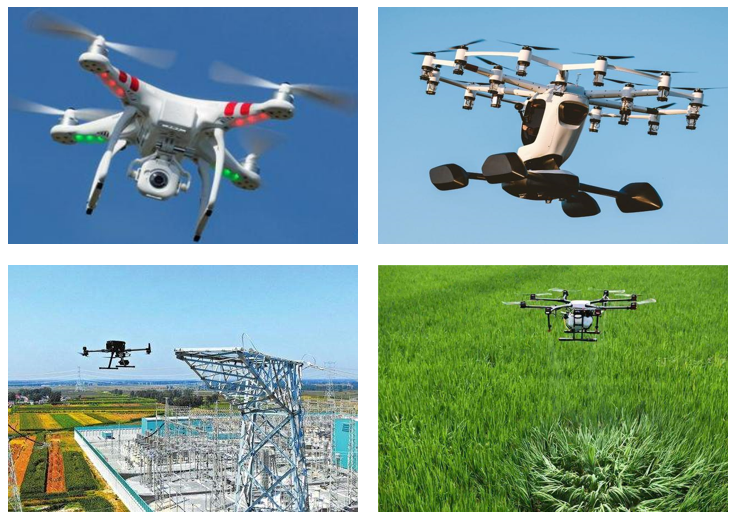
\includegraphics[width=1.0\textwidth]{微信图片_20220506224939.png}
	\bicaption{多旋翼飞行器的在各领域中的应用}{The application of multi-rotor aircraft in various fields}
	\label{fig:Multirotor}
\end{figure}

飞控系统是低成本小型多旋翼飞行器的核心组成部分,其任务是估计飞行器的状态以及控制飞行器的运动。
多旋翼飞行器的飞行性能和飞行安全取决于飞控系统的性能。
对于一般的四旋翼飞行器,标准飞控系统原理框架如\autoref{fig:flightcontrolsystem}所示。
由\autoref{fig:flightcontrolsystem}可见,飞控系统以处理器单元为核心,通过机载传感器获取飞行器的姿态、位置、速度等信息,并根据控制指令对四个电机进行转速调节。
\begin{figure}[H]
	\centering
	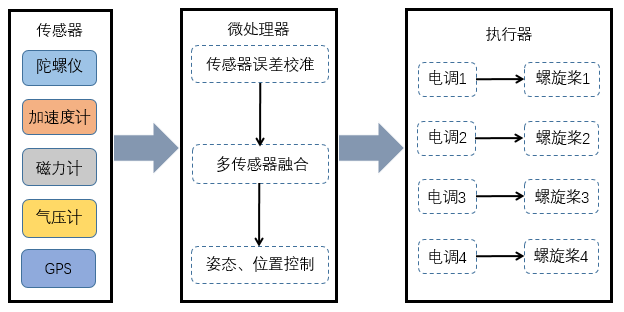
\includegraphics[width=1.0\textwidth]{屏幕截图 2022-06-08 090529.png}
	\bicaption{四旋翼飞行器飞行控制系统结构框图}{Quadrotor aircraft flight control system structure block diagram}
	\label{fig:flightcontrolsystem}
\end{figure}

对于低成本小型多旋翼飞行器来说,飞控系统的状态估计以及运动控制技术是至关重要的。
飞控系统的运动控制通常包括姿态控制、位置/速度控制两部分内容。
其中,姿态控制是运动控制中的重点和难点,也是实现位置、速度控制的基础。
而要实现飞行器的运动控制首先需要知道飞行器的状态。
因此,状态估计是飞行控制系统中首要和最关键的组成部分。

%飞控系统是低成本小型多旋翼飞行器的核心组成部分,其任务是估计飞行器的状态以及控制飞行器的运动。
%多旋翼飞行器的飞行性能和飞行安全取决于飞控系统的性能。
%对于低成本小型多旋翼飞行器来说,飞控系统的状态估计以及运动控制技术是至关重要的。
%
%飞控系统的功能通常包括姿态控制、位置/速度控制两部分功能。
%其中,姿态控制是飞控系统中的重点和难点,也是实现位置、速度控制的基础。
%要实现飞行器的运动控制首先需要知道飞行器的状态。
%对于一般的四旋翼飞行器,标准飞控系统原理框架如\autoref{fig:flightcontrolsystem}所示。
%\begin{figure}[H]
%	\centering
%	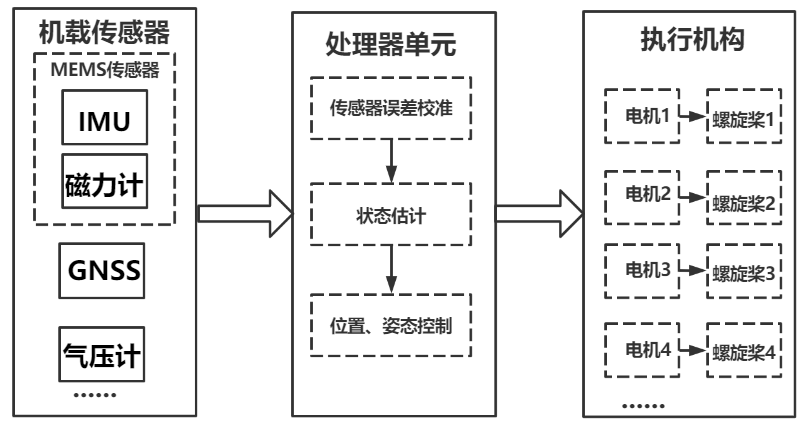
\includegraphics[width=1.0\textwidth]{微信图片_20220504193723.png}
%	\bicaption{四旋翼飞行器飞行控制系统结构框图}{Quadrotor aircraft flight control system structure block diagram}
%	\label{fig:flightcontrolsystem}
%\end{figure}
%
%由\autoref{fig:flightcontrolsystem}可见,飞控系统以处理器单元为核心,通过机载传感器获取飞行器的姿态、位置、速度等信息,并根据控制指令对四个电机进行转速调节。

目前多旋翼飞行器已成功实现商业化,并且有大批科研人员在研究相关的理论和技术\cite{李一博2019微小型飞行器视觉感知与自主导航关键技术研究,cao2015inner,mechali2022fixed}。
但状态估计问题仍然存在许多难题。
一是基于MEMS的IMU的校准问题。
低成本的IMU数据精度较差。
相对于使用高成本的外部设备校准方法而言,低成本且无需外部设备的校准算法是目前研究的重点和热点。
二是多传感器融合问题。
飞行器上通常会搭载IMU、磁力计、气压计、GPS等在内的各种传感器。
其中IMU是多旋翼飞行器最基本的传感器,用于测量飞行器的姿态。
而磁力计则用于测量偏航角,气压计用于测量飞行高度,GPS用于测量飞行器的绝对位置。
一般而言,每个传感器都有其固定的采样频率和延时。
由此引出了如何将多频率和多延时的传感器数据进行融合的问题。
三是传感器扰动抑制问题。
如前所述,多旋翼飞行器上配置了不同的传感器,每个传感器在系统运行过程中都可能受到干扰。
由此引出了如何抑制传感器扰动的问题。

综上所述,对于多旋翼飞行器而言,运动控制中的姿态控制问题和状态估计中的IMU校准、多传感器融合及传感器扰动抑制问题是当前的研究重点。
因此,本课题针对恶劣环境下多旋翼飞行器状态估计的难题,从优化多旋翼飞行器机载IMU传感器性能出发,寻求一融合多频率和多延时的传感器信息的方法,从而有效地提高多旋翼飞行器的状态估计精度及鲁棒性。
本文围绕IMU校准和多传感器数据融合这两个方向上展开研究,并将状态估计与控制结合起来,研发一个完整的飞控系统作为最终目标。
结合相关文献分析\cite{王勇军2021融合多源信息的小型多旋翼无人机位姿估计方法研究},可将本文的研究目的和研究内容归纳为\autoref{fig:research}所示的框图。
\begin{figure}[H]
	\centering
	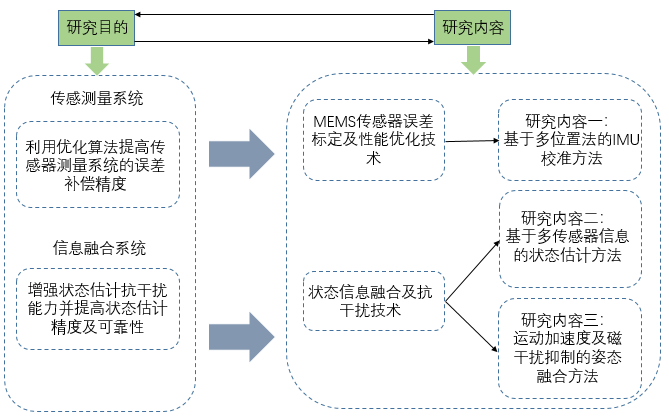
\includegraphics[width=1.0\textwidth]{屏幕截图 2022-06-08 091435.png}
	\bicaption{本课题的研究目的及研究内容关系框图}{The topic research purpose and research content relationship diagram}
	\label{fig:research}
\end{figure}


%在这些场景中,飞行器必须能够自主飞行,以尽量减少操作员的工作量。
%由于多旋翼飞行器具有体积小、悬停能力强、机动性强等优点,其在监视、搜索和救援等场景有很好的应用前景。

%除了上述应用场景外,在人员和地面机器人难以接近或危险复杂环境中,飞行器在监视、搜索和救援任务中具有巨大的潜力。

%在这样的环境中,飞行器要稳定安全地完成作业任务还存在许多挑战。
%首先,所有依赖于单一传感器的方法只能在特定的环境中发挥作用。
%因此,要保证状态估计的稳定性就需要融合更多的传感器,这就引出多源信息融合问题。
%%这里的难点包括如何处理多源信息融合以及如何处理传感器扰动。
%对于多源信息融合问题,由于传感器具有多频率多延时的特性,难点在于算法需要能兼容多个传感器并在不改动程序的情况下能添加或减少传感器。
%其次,每个传感器在运行过程中都有可能受到干扰。
%常见的传感器扰动包括但不限于气压计干扰、磁场干扰、GPS信号异常等。
%飞行器在受到传感器扰动的情况下难以保证安全性。
%对于传感器扰动问题,由于每个传感器的扰动特性不一样,难点在于算法能否有效隔离扰动并不影响状态的连续性。
%再次,飞行器上用的是低成本MEMS传感器,传感器的数据精度限制了状态估计的精度。
%因此需要对传感器进行校准。
%对于传感器校准问题,难点在于在不使用高精度外部设备下对低成本传感器进行校准。
%
%到目前为止,研发一个多旋翼飞行器,并能够在这样的环境中快速自主飞行,需要对状态估计、传感器校准、控制等算法进行综合设计。
%因此,本文将对状态估计、传感器校准和控制这三个问题进行研究。
%其中,状态估计是自主飞行中首要和最关键的组成部分。

\gdutsection{国内外研究现状}{Analysis of the research status at home and abroad}
近年来,人们对应用在多旋翼飞行器的导航与控制算法进行了广泛的研究。
本文回顾了多旋翼飞行器发展过程中出现的一些研究问题及其相关领域的文献。
本节针对IMU校准、多传感器融合、多旋翼飞行控制三个问题的研究现状进行回顾。
\autoref{fig:common}简要概括了这三个问题近年研究较多的主流算法\cite{mahony2008nonlinear,tedaldi2014robust,lee2010geometric,sarkka2017multi,benziane2016attitude,刘烨秋2019基于非线性观测器的飞行器姿态控制方法与应用,王成2018四旋翼无人机飞行控制算法综述,李轾2020两种欠驱动系统的非线性控制方法研究}。
\begin{figure}[H]
	\centering
	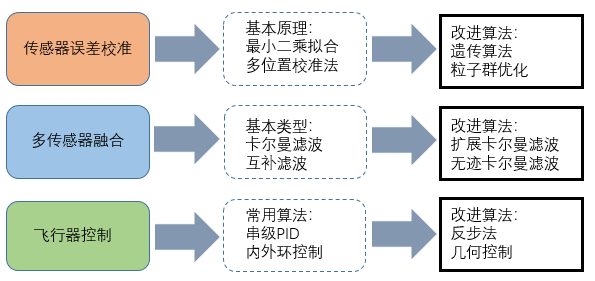
\includegraphics[width=1.0\textwidth]{屏幕截图 2022-06-08 092121.png}
	\bicaption{飞控系统三大环节常用算法概览}{An overview of common algorithms for the three major links of flight control system}
	\label{fig:common}
\end{figure}

\gdutsubsection{IMU校准研究现状}{Research status of IMU calibration}
IMU(惯性测量单元)是机器人工程中常用的传感器。
目前,IMU已被广泛用于惯性导航、姿态估计、视觉惯性导航以及智能手机设备\cite{saha2022tinyodom,qiu2022compensation,jung2022photometric,guo2022robust}。
IMU由一个加速度计和一个陀螺仪组成。
有些IMU还会加入磁力计。
对于一个理想的IMU,三轴传感器应该具备相同的三维正交敏感轴,比例因子应该将每个传感器测量的数字量转换为真实的物理量(如加速度和角速度)。
机器人工程中使用的IMU一般是基于微机电系统技术,简称MEMS。
实际上,基于MEMS的低成本IMU误差通常包括不精确的尺度、传感器敏感轴不对齐和零偏。
IMU校准指的是辨识这些物理量的过程。
对于高精度导航的应用场景,IMU校准的方法是使用成本较高的外部设备来完成。
文献\parencite{hall2000case}具体操作是通过机器人机械臂以一个给定的角速度移动IMU到某个姿态上。
每一次旋转操作结束后,将加速度计的测量值与标准的重力向量进行对比。
而在旋转期间,陀螺仪的测量值与给定的角速度进行对比。
然而,使用机械平台进行校准的方法成本非常高,但实际飞行器中使用的都是廉价的IMU。
文献\parencite{kim2004initial}提出了一种使用光学跟踪系统进行标定的方法,GPS读数用于校准初始偏差和非正交误差。
显然,这些方法的精度非常依赖于所采用的设备的精度,一般会使用运动捕捉系统。
但精度高的运动捕捉系统也十分昂贵。
多位置法最早是文献\parencite{lotters1998procedure}提出的用于实现IMU校准的方法,此方法基于静态加速度的大小必须等于重力的大小这一事实,来校准加速度计的零偏和尺度。
文献\parencite{syed2007new}在文献\parencite{lotters1998procedure}的基础上进行扩展,增加了加速度计轴正交参数。
然而,他们的校准流程需要一个单轴转台。

以上所提到的方法都存在一个缺点:需要一个较精密的外部设备,两个传感器是独立校准的,传感器之间的不对齐无法被检测到。
针对以上不足,Fong等人提出了一种不需要任何外部机械设备的校准方案\cite{fong2008methods}。
与文献\parencite{lotters1998procedure}的方法类似,\parencite{fong2008methods}利用静态加速度的大小必须等于重力的大小这一事实对加速度计进行标定,然后将标定后的加速度计计算的重力向量作为真值,与通过角速度积分得到的重力向量进行对比,得到陀螺仪的标定结果。
文献\parencite{cheuk2012automatic}探讨了磁场的局部稳定性。
Hwangbo等人提出了一种基于迭代矩阵分解的自校准技术,用重力作为加速度计的参考,用相机作为陀螺仪的参考\cite{hwangbo2013imu}。
Tedaldi等人在多位置法的基础上进行改进,提出了一种鲁棒且易于实现的方法来校准IMU,无需任何外部设备\cite{tedaldi2014robust},并且能在优化算法内自动估计静态区间分割的阈值。
本文在文献\parencite{tedaldi2014robust}的基础上,对最优阈值的计算以及参数估计算法进行优化。

\gdutsubsection{多传感器融合研究现状}{Research status of multisensor fusion}
稳定准确地估计一个刚体的状态(即位置和姿态)是机器人实现鲁棒和高性能控制的关键前提。
机器人的状态估计是一个非线性的问题,使用的传感器通常包含非高斯噪声\cite{chen2022nonparametric}。
针对状态估计问题的现有方法有两类,一类是使用扩展的随机线性估计技术\cite{bertsimas2022data,liu2022extended},另一类是使用确定性互补滤波器和非线性观测器设计技术\cite{amor2022three,wang2022nonlinear,wang2022nonlinear}。
在随机线性估计技术中,应用于姿态估计问题的主要算法是扩展卡尔曼滤波(EKF)型方法。
粒子滤波器也被认为是处理非线性的一种方法\cite{wang2022particle}。
由于状态空间的非线性,EKF表现出非鲁棒性和不稳定性\cite{crassidis2007survey}。
相反,非线性观测器利用基础几何来解释问题本质中的非线性。
因此,非线性观测器相比于EKF鲁棒性更强,并具有可证明的几乎全局稳定的性质\cite{thienel2003coupled,mahony2008nonlinear,lageman2009gradient,hua2010attitude,vasconcelos2010nonlinear}。

针对状态估计中的姿态问题,Mahony等人利用旋转的特殊正交群SO(3)的基本李群结构推导了一个互补非线性姿态观测器,并证明了误差系统的几乎全局稳定性\cite{mahony2008nonlinear}。
另一方面,磁场干扰会影响横滚角和俯仰角的估计。
因此,Hua等人考虑了输入信号的解耦,以确保滚转和俯仰估计不受磁场干扰的影响,这是对显式互补滤波器标准实现的一个重要修改,提高了姿态估计的整体质量\cite{hua2011nonlinear}。
此外,大多数现有的姿态观测器/滤波器都依赖于小加速度假设(即$\dot{v}<<g$),因此重力方向测量可以近似于加速度计测量。
然而,许多垂直起降飞行器在快速运动中,飞行器的线性加速度通常是较大的,可能会在姿态估计上产生较大的误差。
针对此问题,Hua等人提出了GPS辅助姿态观测器\cite{hua2010attitude},将GPS线速度的测量值与加速度计的测量值相结合来估计飞行器的加速度,从而提高姿态估计的精度。

以上提到的所有的观测器设计方法都要求对系统的当前输出和输入进行无延迟测量。
然而,在许多实际场景中,系统输出的测量值具有延时(与系统的理想输出比较),而系统输入的测量值可以看作没有延时。
例如,GPS提供的线速度测量值通常相对于飞行器的实际速度是有延时的。
由于各种环境影响和传感器内部处理的延时,延时可以是几百毫秒(甚至半秒)\cite{kingston2004real}。
相比之下,IMU提供的机体角速度和线加速度的测量值几乎是瞬时的。
在状态估计问题中,测量延时会对观测器或滤波器的稳定性和鲁棒性产生负面影响,并降低其性能\cite{battilotti2015nonlinear}。
解决传感器延时问题的经典方法是修改其修正项,使每个延时测量值与相应的后向时移估计值进行比较。
Khosravian等人提出了一种级联观测器-预测器方法来处理李群SO(3)上姿态估计的传感器延时问题\cite{khosravian2016state}。
文献\parencite{khosravian2016state}利用李群SO(3)的代数结构,证明了误差系统的指数收敛性。
结合位置信息,继文献\parencite{mahony2008nonlinear}在SO(3)上的工作之后,Baldwin等人提出了直接在SE(3)上使用全状态反馈和已知特征测量的互补观测器\cite{baldwin2007complementary}。
针对多频率多延时的传感器系统以及传感器异常处理,目前的方法不能很好地解决鲁棒性和安全性问题。

\gdutsubsection{多旋翼飞行控制研究现状}{Research status of multi-rotor flight control}
在获得了飞行器的状态后,可以使用各种现有的控制策略使飞行器稳定飞行。
线性控制器,如PID控制器或LQR控制器,被广泛应用于多旋翼飞行器中\cite{mechali2022fixed,elkhatem2022robust}。
在飞行器工作接近悬停状态的假设下,对于低速运行、加速度变化小的飞行器,可以使用线性控制器。
针对多旋翼飞行器在执行器饱和情况下的线性化动力学问题,Guenard等人设计了一种非线性控制器\cite{guenard2005dynamic}。
文献\parencite{bouabdallah2005backstepping}中应用了反步和滑模技术。
然而,以上所提到的控制器是基于欧拉角设计的,它们在表示多旋翼飞行器复杂的旋转运动时表现出奇点,从而从根本上限制了它们跟踪轨迹的能力。
基于李群上的刚体动力学描述,Lee等人设计了一种应用在四旋翼飞行器的几何控制器,并证明了几乎全局稳定性\parencite{lee2010geometric}。
对于包含大姿态变化的运动,几何控制器是更合适的选择。
本文基于文献\parencite{lee2010geometric}的控制方法进行设计,完成了飞行控制系统的闭环。

\gdutsection{实验平台概述}{Overview of experimental platforms}
本课题研究的一个关键步骤是对提出的算法和系统进行实验验证。
为此,本文使用现成的组件构建了一个多旋翼飞行器平台如\autoref{fig:platform}所示。
\begin{figure}[H]
	\centering
	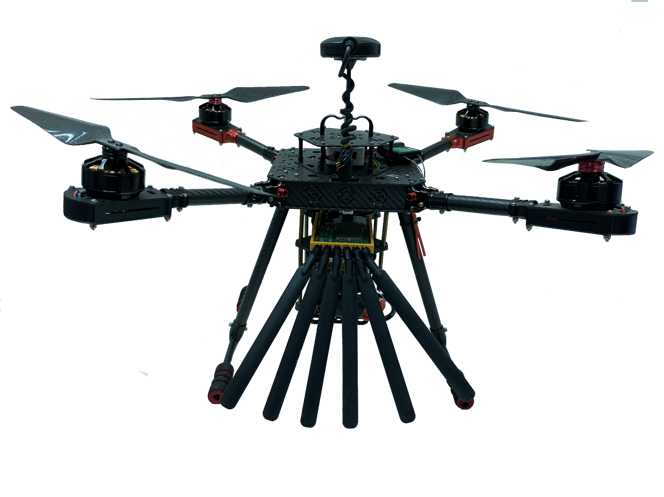
\includegraphics[width=0.92\textwidth]{platform.png}
	\bicaption{实验平台}{Experimental platform}
	\label{fig:platform}
\end{figure} 

飞行器机架材质是碳纤维,具有较好的刚性。
飞行器的主要参数如\autoref{Mainparametersofaircraft}所示。
\begin{table}[h]
	\bicaption{飞行器主要参数}{Main parameters of aircraft}
	\label{Mainparametersofaircraft}
	\begin{tabular}{ccccc}
		\toprule
		起飞重量($g$) & 轴距($mm$) & 桨叶尺寸($inches$)\\
		\midrule
		1150 & 450 & 9 \\ 
		\bottomrule 
	\end{tabular}
\end{table}

实验平台上安装的飞控板如\autoref{fig:AutoPilotboard}所示,本文在这个飞控板上实现算法。
飞控板由IMU、磁力计、气压计和用户可编程的STM32微控制器组成。
\begin{figure}[H]
	\centering
	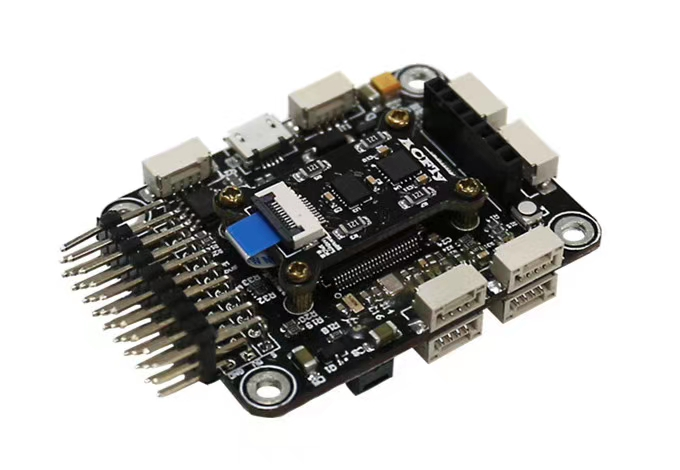
\includegraphics[width=0.8\textwidth]{acfly.jpg}
	\bicaption{飞控板}{AutoPilot board}
	\label{fig:AutoPilotboard}
\end{figure}

微控制器采用的STM32H743VIT6如\autoref{fig:STM32H743VIT6}所示,主频高达480M,有16Kb的L1级缓存Cache,1M内存,2M Flash,支持硬件双精度浮点运算。
\begin{figure}[H]
	\centering
	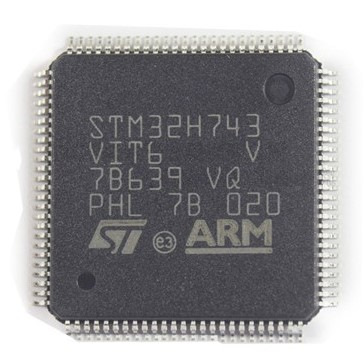
\includegraphics[width=0.3\textwidth]{St-Semiconductor-Chips-Electronic-Component-Lqfp-100-Stm32h743vit6.jpg}
	\bicaption{STM32H743VIT6}{STM32H743VIT6}
	\label{fig:STM32H743VIT6}
\end{figure}

IMU芯片采用BMI088,如\autoref{fig:BMI088}所示。
BMI088是一款高性能六轴惯性测量单元,具有高振动稳定性,专为无人机和机器人应用而设计。
BMI088具有出色的抗振性和抑制能力,可在较大的温度变化下保持稳定。
BMI088的加速度计量程最大是24g,陀螺仪的最大量程是2000°/s。
即使在大震动环境下也不会超量程。
\begin{figure}[H]
	\centering
	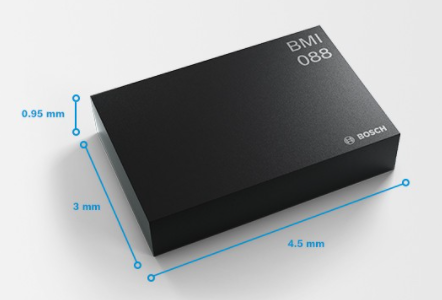
\includegraphics[width=0.46\textwidth]{屏幕截图 2022-03-30 151212.png}
	\bicaption{BMI088}{BMI088}
	\label{fig:BMI088}
\end{figure}

磁力计采用AK8975,气压计采用SPL06。
对于位置传感器,使用ublox的GPS模块。
本文中讨论的所有算法都是用C++实现,运行在如\autoref{fig:AutoPilotboard}所示的飞控板上。

\gdutsection{本文研究内容及安排}{Thesis contributions and overview}
论文结合多旋翼飞行器状态估计精确性和稳定性的需求,从IMU误差校准补偿和传感器可靠融合两方面出发,采用实验验证方法来开展研究工作。
本文主要针对基于多位置法的IMU校准方法、基于多频率和多延时的状态估计方法以及基于运动加速度及磁场干扰的传感器融合方法展开研究。
论文组织架构如\autoref{fig:blockdiagram}所示。
\begin{figure}[H]
	\centering
	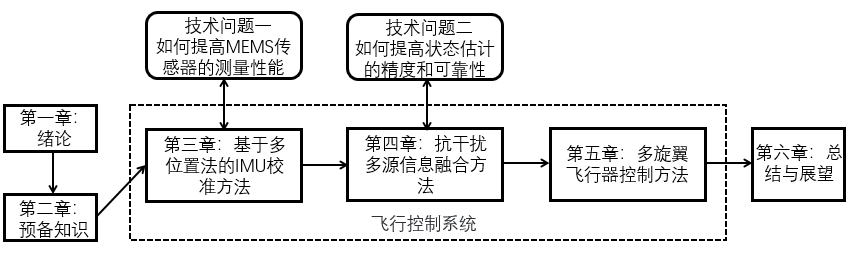
\includegraphics[width=1.0\textwidth]{屏幕截图 2022-05-05 153942.png}
	\bicaption{论文研究内容与研究框图}{Research content and block diagram}
	\label{fig:blockdiagram}
\end{figure}

%本文的研究工作在于多旋翼飞行器自主飞行相关算法的开发。
%首先,提出了预测-修正-延时融合框架,以处理多频率多延时的传感器系统。
%然后,对每个传感器的特性进行研究,针对磁场干扰及运动加速度补偿进行优化处理,以提高系统的鲁棒性。
%其次,进一步优化了IMU校准算法,提出了新的最优阈值的算法,提高了IMU本身输出数据的精度。
%最后,整合了控制算法,形成一个完整的飞行控制系统。
论文由六个章节组成,每个章节的安排如下:

第一章为绪论,详细介绍本课题的研究背景与关键技术问题,调查了多旋翼飞行器的发展现状,介绍了飞行控制系统中的三个关键问题,分别对IMU校准、多传感器融合、多旋翼飞行控制问题的研究现状进行了详细介绍,并阐述了本文的主要贡献和论文的结构安排。

第二章为预备知识,介绍了坐标系定义、姿态表示、刚体运动学、传感器模型等基础知识。

第三章给出了多旋翼飞行器IMU校准算法方法。
首先分析了IMU的误差,给出了IMU误差模型,并对基于多位置法的IMU校准算法研究分析,进一步优化了IMU校准算法,提出了新的最优阈值的算法,提高了IMU本身输出数据的精度。

第四章研究了抗干扰多源信息融合方法。
围绕状态估计问题展开研究,提出了预测-修正-延时融合框架,以处理多频率多延时的传感器系统。并且对每个传感器的特性进行研究,针对磁场干扰及运动加速度补偿进行优化处理,以提高系统的鲁棒性。

第五章介绍了多旋翼飞行器控制方法。整合了现有控制方法,以满足飞行器稳定飞行的需求,形成一个完整的飞行控制系统。

第六章为总结与展望。
最后对研究工作进行总结并提出了未来的研究方向。

\gdutchapter{预备知识}{Preliminaries}

%\gdutsection{状态估计相关基础知识}{Basic knowledge of state estimation}

状态估计的目标是输出飞行器六自由度的状态。
状态包括三自由度的位置和三自由度的姿态。
本章给出算法推导的一些预备知识,包括坐标系定义、姿态表示、刚体运动学和传感器模型。

%多旋翼飞行器采用多个传感器组成状态估计系统。
%为了实现稳定飞行,需要实时获取飞行器的当前姿态、速度与位置等参数。
%为描述多旋翼飞行器的姿态和位置,必须建立适当的坐标系,以便于理清变量之间的关系。
%同时,将多旋翼无人机看成刚体,用数学语言描述其姿态以及刚体运动学。
%最后给出传感器模型。

\gdutsection{坐标系定义}{Coordinate system definition}
% note 分段
飞行器的位置、速度都可以抽象成三维向量,这就需要定义坐标系。
一般会选择三个相互正交的三维向量来构成直角坐标系。
首先定义两个坐标系,一个世界坐标系(inertial frame),一个机体坐标系(body frame)。
将世界坐标系记为$W$,将机体坐标系记为$B$。
其中,$W$系是静止的参考坐标系,而$B$系是运动坐标系。
\begin{figure}[htbp]
	\centering
	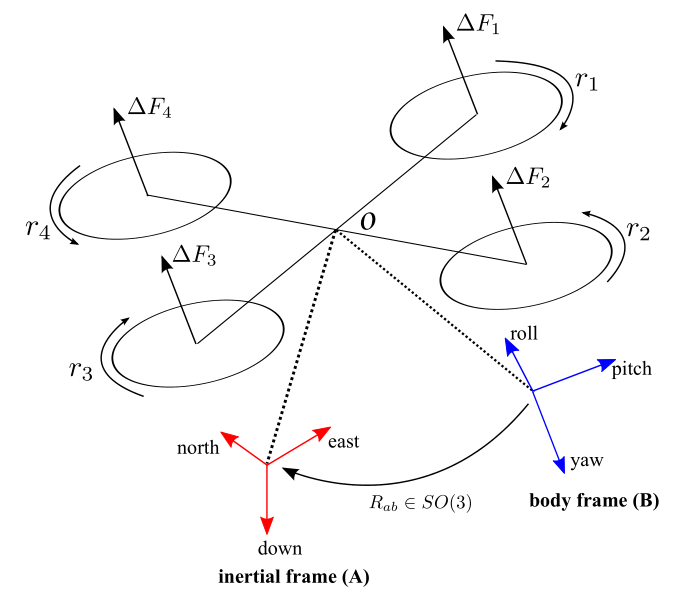
\includegraphics[width=0.8\textwidth]{屏幕截图 2022-03-31 222546.png}
	\bicaption{飞行器模型}{The model of the aerial robot}
	\label{fig:modelaerialrobot}
\end{figure}

如\autoref{fig:modelaerialrobot}所示,定义$W$系原点在飞机初始点,为北-东-地坐标系,$B$系原点在飞行器质心,$x$轴指向机头、$y$轴指向右侧,$z$轴指向下方。将世界坐标系的三个坐标轴记为$\big\{ \vec{e}_1,\vec{e}_2,\vec{e}_3 \big\}$,机体坐标系的三个坐标轴记为$\big\{ \vec{b}_1,\vec{b}_2,\vec{b}_3 \big\}$。
接着,再定义一个坐标系:
其坐标原点位于飞行器质心,$z$轴轴垂直于地面并指向地心,$x$轴与机体系$\vec{b}_1$轴在水平面内的投影重合,$y$轴与机体系$\vec{b}_2$轴在水平面内的投影重合。此坐标系记位$bodyheading$坐标系。
这样,飞行器的位置向量,速度向量,加速度向量,角速度向量就都有了可以表示的坐标系。
使用上标的方式描述状态量所投影的坐标系,将世界坐标系和机体坐标系中的向量分别定义为$(\cdot)^w$和$(\cdot)^b$。
用$p^w$、$v^w$、$a^w$分别表示世界坐标系中飞行器的位置、速度、加速度。

\gdutsection{姿态表示}{Attitude representation}
% note 分点
姿态是描述两个坐标系之间的相对关系。
目前有四种流行的姿态表示法,分别是欧拉角、旋转矩阵、四元数和旋转矢量\cite{shuster1993survey}。

在众多姿态表示方法中,欧拉角的应用最为广泛\cite{stuelpnagel1964parametrization}。
欧拉角可以将姿态表示为三个角度。
如\autoref{fig:eulerangle}所示,定义机体坐标系与世界坐标系之间的夹角为飞机的姿态角,又称欧拉角:
\begin{itemize}
	\item 俯仰角$\theta$:机体轴与地平面(水平面)之间的夹角,飞机抬头为正。
	\item 偏航角$\psi$:机体轴在水平面上的投影与地轴之间的夹角,以机体右偏为正。
	\item 横滚角$\phi$:飞机对称面绕机体轴转过的角度,右滚为正。
\end{itemize}
\begin{figure}[H]
	\centering
	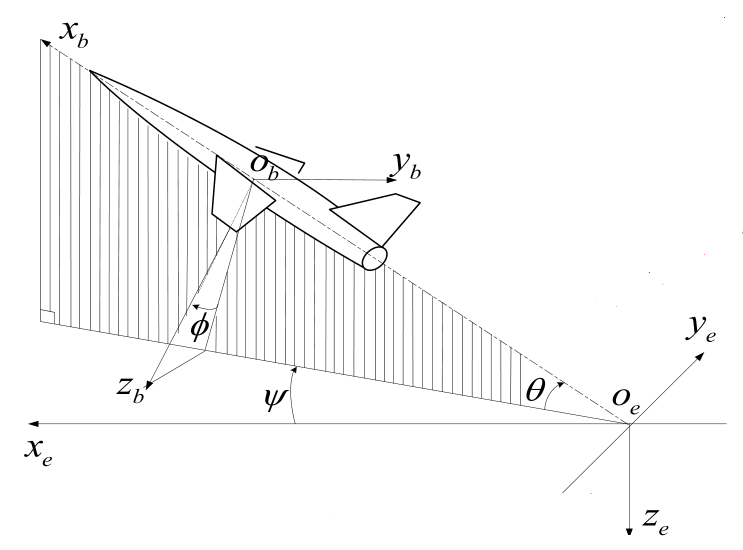
\includegraphics[width=0.7\textwidth]{屏幕截图 2022-03-31 231147.png}
	\bicaption{欧拉角示意图}{Schematic diagram of euler angle}
	\label{fig:eulerangle}
\end{figure}
三维旋转具有三个自由度。
欧拉角是所有姿态的表示方法中需要用到参数最少的一种,也就是只用到三个参数。
但是,当俯仰角$\theta \pm \frac{\pi}{2}$时,欧拉角存在自锁现象(gimbal lock)。
在自锁点附近,横滚角$\phi$及航向角$\psi$的导数会趋向于无穷大,这也是欧拉角表示方法的奇异点。
因此,不需要在算法中使用欧拉角进行运算。
接下来本文引入旋转矩阵。

如\autoref{fig:modelaerialrobot},可以用坐标系$W$的坐标轴表示坐标系$B$的基。
记坐标系$B$的基坐标为$x_{wb}, y_{wb}, z_{wb} \in \mathbb{R}^3$。
定义旋转矩阵
\begin{equation}\label{eq:rotationmatrixdefinition}
	R_b^w = 
	\begin{bmatrix}
		x_{wb} & y_{wb} & z_{wb}
	\end{bmatrix}
\end{equation}
表示坐标系$B$相对于坐标系$W$的姿态。
可以证明两个旋转矩阵的乘积还是旋转矩阵,所以全部旋转矩阵构成一个“群”,也就是SO(3)群,其定义为
\begin{equation}\label{eq:so3}
	SO(3) \triangleq \left\{ R \in \mathbb{R}^{3 \times 3} | det(R) = 1, R^T R = R R^T = I_3 \right\}
\end{equation}
旋转矩阵用了九个参数去表示三个自由度的姿态。
显然可以用更少的参数去表示姿态,接下来本文引入旋转矢量。

根据欧拉旋转定理,任何一个三维旋转可以表示为绕一根转轴$u$旋转一个角度$\theta$,其中转轴$u$是单位向量\cite{palais2007euler}。
因此最直接的姿态的表示方法是单位向量$u$和角度$\theta$,这种方法被称为欧拉轴-角(axis-angle)。
为了一些计算上的方便,可以把轴和角相乘,得到一个三维空间内的一般向量$u\theta$。
很容易验证$u\theta$和欧拉轴-角是一一对应的,这就是姿态的另一种表示方法,即旋转矢量。
最后需要说明的是,当$\theta = 2\pi$时,旋转矢量$u\theta$的导数会出现无穷大的情况,这是旋转矢量表示方法的奇异点。
接下来本文引入四元数。

四元数是对复数数系的进一步拓展,由四个实数表示:
\begin{equation}\label{eq:quatdef1}
	q = q_w + q_x i + q_y j + q_z k \triangleq 
	\begin{bmatrix}
		q_w & q_x & q_y & q_z
	\end{bmatrix}
\end{equation}
根据旋转矢量直接给出四元数另一种定义,表示一个三维旋转的单位四元数可以由旋转矢量$u\theta$计算得到:
\begin{equation}\label{eq:quatdef}
	q(u,\theta) = 
	\begin{bmatrix}
		cos(\frac{\theta}{2}) \\
		u_x sin(\frac{\theta}{2}) \\
		u_y sin(\frac{\theta}{2}) \\
		u_z sin(\frac{\theta}{2})\vspace{1ex}
	\end{bmatrix}	
\end{equation}
\vspace{1ex}这种定义方式有旋转的物理含义。
四元数最常见的运算是四元数乘法:
\begin{equation}
	p \otimes q = 
	\begin{bmatrix}
		p_w q_w - p_x q_x - p_y q_y - p_z q_z \\
		p_w q_x + p_x q_w + p_y q_z - p_z q_y \\
		p_w q_y - p_x q_z + p_y q_w + p_z q_x \\
		p_w q_z + p_x q_y - p_y q_x + p_z q_w \vspace{1ex}
	\end{bmatrix}	
\end{equation}
其中,$p$和$q$是两个四元数,$\otimes$记为四元数乘法。
四元数相乘的物理意义是旋转叠加,这个性质在本文的算法设计中使用。

另外,将$\theta + 2\pi$代入\autoref{eq:quatdef}可以得到$q(u,\theta + 2\pi)=-q(u,\theta)$,这意味着$q$和$-q$表示相同的三维旋转。
这是单位四元数一个非常重要的性质,它和三维旋转并不是一一对应的,而是2比1的对应关系。

以上是刚体的姿态表示方法:旋转矢量、旋转矩阵、四元数和欧拉角。
刚体的姿态有三个自由度,在四种表示方法中,旋转矢量和欧拉角用了三个参数。
四元数用了四个参数和一个约束条件(长度为1)。
旋转矩阵用了九个参数和六个约束条件(矩阵的正交性)。
旋转矢量和欧拉角都具有奇异性,也就是说在某种姿态下,它们的导数会趋向无穷大。
四元数没有奇异性,但它和姿态是2比1的对应关系。
只有旋转矩阵既没有奇异性,而且和姿态是一一对应的。
在姿态估计中,可以使用旋转矩阵、四元数或欧拉角对角速度进行积分,并设计滤波器。
实际上,本文的算法中使用的状态量是以四元数表示,但是计算过程会涉及到各种表示的转换。

\gdutsection{刚体运动学}{Rigid body kinematics}
对于飞行器,可以将其看作三维空间的一个刚体。
刚体运动学是设计观测器的基本方程。
使用旋转矩阵表示,刚体姿态运动学可以用如下方程描述
\begin{gather}\label{eq:matrixkinematics}
	\dot{R}=R (\omega)_{\times}
\end{gather}
其中$R$为刚体的姿态。$(\omega)_{\times}$为反对称矩阵,其定义为
\begin{gather}\label{eq:matrixkinematics}
	(\omega)_{\times}=
	\begin{bmatrix}
		0 & -\omega_z & \omega_y\\
		\omega_z & 0 & -\omega_x\\
		-\omega_y & \omega_x & 0\vspace{1ex}
	\end{bmatrix}
\end{gather}
\vspace{1ex}使用四元数表示,刚体姿态运动学可以用如下方程描述
\begin{gather}\label{eq:quatkinematics}
	\dot{q}=\frac{1}{2} q \otimes \mathbf{p}(\omega)
\end{gather}
其中$q$为刚体的姿态,$\mathbf{p}(\omega)=(0,\omega)$是纯四元数,此处的物理意义是姿态的速度。
刚体位置运动学可以用如下方程描述,其中$p$为刚体的位置。
\begin{gather}\label{eq:matrixkinematics}
	\dot{p}=v
\end{gather}

\gdutsection{传感器模型}{Sensor model}
本文在多旋翼飞行器上配置的传感器有IMU(陀螺仪+加速度计)、磁力计、GPS、气压计。
其中,最基本的传感器是MEMS IMU。
一般的IMU由一个三轴陀螺仪和一个三轴加速度计组成。

三轴陀螺仪测量的是角速度$\omega$,其模型为
\begin{equation}\label{eq:gyromodel}
	\omega_y=\omega+b_w+\eta_w
\end{equation}
其中$\omega \in B$,$\eta_w$是测量噪声,$b_w$表示一个恒定或缓慢时变的陀螺零偏。
一般来说,陀螺仪对噪声不敏感,在飞行器应用中相当可靠。

三轴加速度计测量的去掉重力后的整体加速度,其模型为
\begin{equation}\label{eq:accmodel}
	a_y=R^T(\dot{v}-g)+b_a+\eta_a
\end{equation}
其中$\eta_a$表示测量噪声,$b_a$表示加速度零偏,$\dot{v}$是世界系的加速度。
加速度计对振动十分敏感。
因此,通常需要对加速度数据进行较大的低通滤波后才能使用。

三轴磁力计测量的是磁场强度,其模型为
\begin{equation}\label{eq:magmodel}
	m_y=R^T m^w+B_m+\eta_m
\end{equation}
其中$m^w$为在世界系的地球磁场矢量,$B_m$为局部磁场干扰,$\eta_m$为测量噪声。
$B_m$表示由电机和电流产生的所有内部磁场扰动以及外部磁场的总和。
$\eta_m$通常是比较小的。
但是,如果传感器被放置在电机的电源线附近,局部磁场干扰$B_m$可能是非常大的。

气压计和GPS作为位置传感器,其模型为
\begin{equation}\label{eq:magmodel}
	z_y=z^w+b+\eta
\end{equation}
其中$z^w$是世界系的位置向量,$\eta$是测量噪声。

\gdutchapter{基于多位置法的IMU校准方法}{IMU calibration method based on multi-position method}
%基于微机电系统(MEMS)的IMU具有低成本、体积小、低功耗等优点。
%然而对于低成本MEMS的IMU,其零偏、尺度、非正交及温漂等误差远大于高精度惯性导航器件。
%因此,基于MEMS的IMU校准有很好的研究价值。
多旋翼飞行器的精准作业对导航精度有非常高的要求,导航精度的上限是取决于传感器数据精度的上限。
然而,基于MEMS的传感器的精度都比较差,远远达不到高精度导航的要求。
%然而,飞行器的精准作业对导航精度有非常高的要求。
因此,提高传感器数据精度是非常关键的一环。

在前人工作的基础上,本章开发了一种不需要外部设备就可以进行较高精度的校准算法,提出了新的最优阈值的计算方法,能避免采样数较少导致校准精度下降的情况。
要求校准算法能够使用人手就能完成,无需外部设备,在尽量简单的校准流程下保证校准结果的准确性。

%\gdutsection{问题描述}{Problem formulation}
%基于MEMS的低成本IMU误差通常包括不精确的尺度、传感器敏感轴不对齐和零偏的影响。
%IMU校准指的是辨识这些物理量的过程。
%首先用数学语言描述这些待求参数。

\gdutsection{传感器误差模型}{Sensor error model}
本文第二章已经对传感器建立了数学模型,但这个模型是校准后的模型。
下面描述的是校准前的模型。

对于一个理想的IMU,三轴传感器应该具备相同的三维正交敏感轴,比例因子应该将每个传感器测量的数字量转换为真实的物理量,如加速度和角速度。
实际上,基于MEMS的低成本IMU误差通常包括不精确的尺度、传感器敏感轴不对齐和零偏。
轴正交误差可以建模成一个矩阵
\begin{equation}\label{eq:axiserror}
	T=
	\begin{bmatrix}
		1 & \beta_{yz} & \beta_{zy}\\
		\beta_{xz} & 1 & \beta_{zx}\\
		\beta_{xy} & \beta_{yx} & 1
	\end{bmatrix}\vspace{1ex}
\end{equation}
其中,$T$是轴正交矩阵,$\beta_{ij}$是第$i$个传感器轴的误差对第$j$个轴的造成的误差影响。
比例因子误差可以建模成一个对角阵
\begin{equation}\label{eq:scaleerror}
	K=
	\begin{bmatrix}
		s_x & 0 & 0\\
		0 & s_y & 0\\
		0 & 0 & s_z
	\end{bmatrix}
\end{equation}
零偏可以建模成一个向量
\begin{equation}\label{eq:scaleerror}
	b=
	\begin{bmatrix}
		b_x\\
		b_y\\
		b_z
	\end{bmatrix}
\end{equation}
完整的传感器误差模型为
\begin{equation}\label{eq:sensorerrormodel}
	x^O=T K (x^S + b + \nu)
\end{equation}
其中,$x$指一种三轴传感器,$x^O$和$x^S$分别表示校准后和校准前的传感器数据,$ν$是传感器测量噪声。
那么可以由\autoref{eq:sensorerrormodel}写出加速度计和陀螺仪的误差模型。
其中,加速度计的误差模型为
\begin{equation}
	a^O=T^a K^a (a^S + b^a + \nu^a)
\end{equation}
陀螺仪的误差模型为
\begin{equation}\label{eq:accerrormodel}
	\omega^O=T^\omega K^\omega (\omega^S + b^\omega + \nu^\omega)
\end{equation}
从而,也得到需要求解的参数,将这些参数定义为
\begin{equation}\label{eq:thetadef}
	\theta = 
	\begin{bmatrix}
		\beta_{yz},\beta_{zy},\beta_{xz},\beta_{zx},\beta_{xy}, \beta_{yx},s_x,s_y,s_z,b_x,b_y,b_z
	\end{bmatrix}
\end{equation}
那么可以由\autoref{eq:thetadef}写出加速度计和陀螺仪的待求参数。
其中,加速度计的待求参数向量为
\begin{equation}
	\theta^a = 
	\begin{bmatrix}
		\beta_{yz}^a,\beta_{zy}^a,\beta_{xz}^a,\beta_{zx}^a,\beta_{xy}^a, \beta_{yx}^a,s_x^a,s_y^a,s_z^a,b_x^a,b_y^a,b_z^a
	\end{bmatrix}
\end{equation}
陀螺仪的待求参数向量为
\begin{equation}
	\theta^\omega = 
	\begin{bmatrix}
		\beta_{yz}^\omega,\beta_{zy}^\omega,\beta_{xz}^\omega,\beta_{zx}^\omega,\beta_{xy}^\omega, \beta_{yx}^\omega,s_x^\omega,s_y^\omega,s_z^\omega,b_x^\omega,b_y^\omega,b_z^\omega
	\end{bmatrix}
\end{equation}

\gdutsection{传统校准算法分析}{Analysis of traditional calibration algorithms}
将校准问题用数学语言表述之后,本节将讨论具体的算法实现,分析各种算法的优劣以及目前存在的问题,以引出本文的设计。

\gdutsubsection{外部设备法}{External equipments}
对于高精度导航的应用场景,IMU校准的方法是使用成本较高的外部设备来完成的,如机器人机械手。
具体操作是以一个给定的角速度移动IMU到某个姿态上\cite{hall2000case}。
对于每一次旋转操作,将加速度计的测量值与标准的重力向量进行对比,而在旋转期间,陀螺仪的测量值与给定的角速度进行对比。
然而,使用校准的机械平台成本非常高,但实际飞行器中使用的都是廉价的IMU。

%IMU校准的传统方法是通过使用特殊的机械平台来完成的,如机器人机械手、转台。
%具体操作是以已知的旋转速度移动IMU到精确控制的姿态上\cite{hall2000case}。
%在每个姿态上,加速度计的输出与预先计算的重力向量进行比较,而在旋转期间,陀螺仪的输出与预先计算的旋转速度进行比较。
%然而,用于校准的机械平台通常非常昂贵,导致校准成本往往超过IMU的硬件成本。

\gdutsubsection{多位置法}{Multi-position method}
多位置法最早是由Lotters等人提出的\cite{lotters1998procedure}。
Lotters等人提出,利用静态加速度的大小必须等于重力的大小这一事实,来校准加速度计的零偏和尺度。
所有参数都可以通过在一组静态姿态上最小化残差来估计。
在校准完加速度计后,可以利用加速度计测量到的重力矢量位置作为基准来校准陀螺仪。
积分两个连续静止位置之间的角速度,可以估计在新位置上的重力向量。
最终通过这些估计值与校准后的加速度计给出的重力参考值之间的误差最小化来校准陀螺仪。
此方法可在无外部设备情况下应用于低成本IMU校准上。

\gdutsection{基于多位置法的IMU校准算法设计}{Design of IMU calibration algorithm based on multi-position method}
本节描述一种校准IMU的方法,以提高IMU本身的数据精度。
这项工作的主要目标是开发一种无需外部设备,只需要用手移动传感器,并将其置于一组不同的静态位置(姿态),通过简单的流程就能实现校准。
本文的关键贡献是一种基于\parencite{tedaldi2014robust}的方法,提出了新的最优阈值算法,改进了参数估计算法,提高了IMU本身输出数据的精度。

\gdutsubsection{校准流程}{Calibration procedure}
本文的校准流程需要收集加速度计和陀螺仪的原始数据的数据集。
首先,静止放置IMU一段时间。
接着,操作员需要将IMU移动到不同的姿态时,产生了一组明显的、稳定的旋转,同时保持每个静态间隔的持续时间,以满足陀螺仪零偏不变的假设。
旋转足够多次数后即完成校准流程。
完整的IMU校准流程如\autoref{fig:Flowchartofcalibration}所示。
%记校准流程中IMU旋转的姿态次数为N。
%为了避免校准参数估计中的不可观性,至少需要收集12组不同姿态的。
%一般来说,N越大,校准结果越好。
%同时保持每个静态间隔的持续时间,以满足陀螺仪零偏不变的假设。
%参数估计算法后面给出伪代码。
%IMU校准流程如\autoref{fig:Flowchartofcalibration}。
\begin{figure}[H]
	\centering
	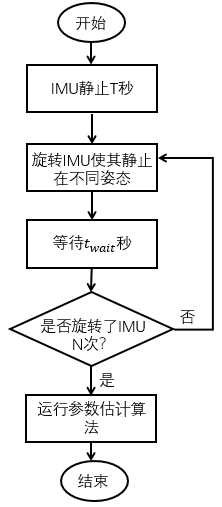
\includegraphics[width=0.36\textwidth]{屏幕截图 2022-06-08 104040.png}
	\bicaption{校准流程图}{Flow chart of calibration}
	\label{fig:Flowchartofcalibration}
\end{figure}
其中,$t_{wait}$是每个静态区间的最大长度,$T$是初始化静止时间,$N$是旋转IMU到不同姿态的次数,为了避免校准参数估计中的不可观性,至少需要收集12组不同姿态。
%一般来说,N越大,校准结果越好。

\gdutsubsection{非线性优化}{Nonlinear optimization}
采集了IMU的数据集后,可以通过数据集来求解校准参数。
接下来使用非线性优化的方法估计IMU参数。
首先需要定义加速度计和陀螺仪的代价函数。

定义函数为
\begin{equation}
	a^O=h(a^S,\theta^a) =T^a K^a (a^S + b^a)
\end{equation}
对于加速度计的误差模型,可以将噪声项忽略不计,这是因为在校准程序中,算法对每个静态区间的加速度信号求均值。
记录$N$组稳定的姿态,在每个静态间隔内的一个时间窗口内平均加速度计读数可以提取$M$个加速度矢量$a^S_k$。
定义加速度计校准参数的代价函数为
\begin{equation}\label{eq:costacc}
	L(\theta^a)=\sum_{k=1}^{M}(\left\|g\right\|-\left\|h(a^S,\theta^a)\right\|)^2
\end{equation}
其中,$\left\|g\right\|$是当地重力向量的模长。
为了使\autoref{eq:costacc}最小化,使用Levenberg-Marquardt算法求解$\theta^a$。

对于陀螺仪校准,由初始静止阶段可以计算出零偏,因此可以假设陀螺仪是无偏的。
此外,由于需要使用校准后的加速度计作为真值,因此使用上面计算的校准参数$\theta^a$,用\autoref{eq:accerrormodel}对加速度计读数进行校准。

由陀螺仪数据在一段时间内积分出旋转,可以计算出结束位置的重力矢量。
定义函数
\begin{equation}\label{eq:integration}
	u_{g,k}=\phi(\omega^S_i , u_{a,k-1})
\end{equation}
其中,$\omega^S_i$是$n$个陀螺仪读数的序列,$u_{a,k-1}$是一个初始重力矢量,$u_{g,k}$是终点重力矢量,$\phi$是通过对角速度进行积分来计算最终位置的计算方法。
在这种情况下,定义代价函数为
\begin{equation}\label{eq:costgyro}
	L(\theta^\omega)=\sum_{k=2}^{M}(u_{a,k}-u_{g,k})^2
\end{equation}
同理,使用LM算法最小化\autoref{eq:costgyro}求解$\theta^\omega$。

\gdutsubsection{静态检测}{Static detector}
采集数据的过程包括运动状态和静止状态,需要将不同状态的数据区分开来。
静态检测的作用是对采集过程进行分割,进而区分静态区间和运动区间。
本文中加速度计的校准采用静态区间的数据,而陀螺仪的校准采用两个连续静态区间之间的运动区间的数据。

基于带通滤波器的算法,比如\parencite{fong2008methods}中使用的准静态检测器,在实际数据集上表现很差。
这类算法检测到的静态区间经常包含一小部分运动。
此外,它们还需要进行微调,因为算法依赖于三个参数。
本算法的检测器是基于Tedaldi的方法\cite{tedaldi2014robust}。
对于每个加速度计样本$\begin{bmatrix}
	a^t_x & a^t_y & a^t_z
\end{bmatrix}$,给定一个长度为$t_{wait}$秒的时间间隔时刻,计算方差的大小
\begin{equation}\label{eq:var}
	\zeta(t)=\sqrt{[var_{t_w}(a^t_x)]^2+[var_{t_w}(a^t_y)]^2+[var_{t_w}(a^t_z)]^2}
\end{equation}
其中$var_{t_w}(a^t)$是一个运算符,计算加速度计$a^t$在以$t$为中心,长度为$t_w$秒的时间间隔内的方差。
通过判断$\zeta(t)$是否小于或大于一个阈值对静态和运动区间进行分割。
作为阈值,考虑方差大小平方$\zeta_{init}$的整数倍。
其中,$\zeta_{init}$是初始化阶段的方差。
需要注意的是,Tedaldi的静态检测器不需要调参。
检测器能依据某种原则自动估计出阈值。
而本文将提出一种新的阈值估计算法。
\autoref{fig:staticdetection}显示了静态检测是如何处理真实数据的。
其中,红绿蓝信号是加速度计三轴原始数据。
静态检测器由紫色方波表示,它的高电平是一个静态区间。
\begin{figure}[H]
	\centering
	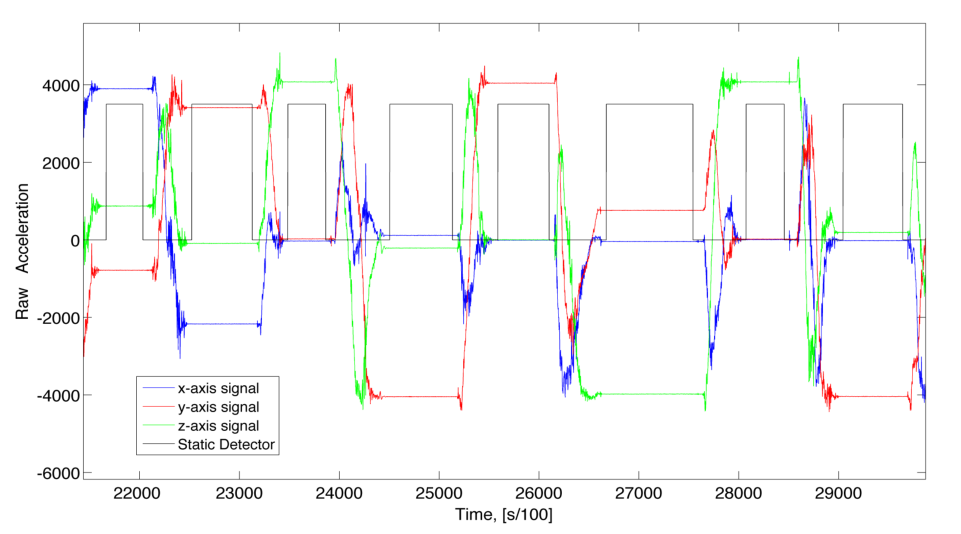
\includegraphics[width=1.0\textwidth]{屏幕截图 2022-04-03 103640.png}
	\bicaption{静态检测示意图}{Diagram of static detection}
	\label{fig:staticdetection}
\end{figure}

\gdutsubsection{龙格-库塔积分}{Runge-Kutta Integration}
如\autoref{eq:integration}所述,在陀螺仪校准中,需要对离散时间角速度进行积分。
本文采用一种鲁棒且稳定的数值积分方法以提高校准精度。
龙格-库塔法是一种常用的数值积分算法\cite{andrle2013geometric}。
四阶龙格-库塔法(RK4n)优于标准的线性积分算法,输出更高精度的结果。
因此,本文采用四阶龙格-库塔法对角速度进行积分。
定义四元数运动学的微分方程为
\begin{equation}
	\dot{q}(k)=f(\cdot )=\frac{1}{2} q \otimes \mathbf{p}(\omega_y(k))
\end{equation}
RK4n积分算法为
\begin{equation}\label{eq:rk4}
	\begin{aligned}
		q_{k+1} &= q_k + \frac{\Delta t}{6}(k_1 + 2 k_2 + 2 k_3 + k_4)\\
		k_1 &= f(t_k , q_k)\\
		k_2 &= f(t_k + \frac{\Delta t}{2},q_k + \frac{\Delta t}{2} k_1)\\
		k_3 &= f(t_k + \frac{\Delta t}{2},q_k + \frac{\Delta t}{2} k_2)\\
		k_4 &= f(t_k + \Delta t, q_k + \Delta t k_3)\vspace{1ex}
	\end{aligned}
\end{equation}
最后,对于每一次迭代,还需要对$k+1$时刻四元数进行归一化处理
\begin{equation}
	q_{k+1} = \frac{q_{k+1}}{\left\|q_{k+1}\right\|}
\end{equation}

\gdutsubsection{IMU参数估计算法}{IMU parameter estimation algorithm}
本节前面介绍了非线性优化、静态检测以及龙格库塔积分算法,接下来将上述环节组合起来形成完整的参数估计算法。本文在此基础上提出新的阈值计算方法。

首先通过校准流程采集到加速度计和陀螺仪的数据集。
然后在初始化阶段可以算出陀螺仪的零偏$b^\omega$以及通过\autoref{eq:var}计算$\zeta_{init}$。
根据文献\parencite{tedaldi2014robust}描述的算法,通过$\zeta_{init}$的整数倍设置阈值,检测静态区间,最小化\autoref{eq:costacc},根据残差和的大小来选取最优的阈值。
但从原理上,残差和其实不仅和校准的效果有关,与样本数量也有关系。
样本数量越少,计算的残差和越小。
但在样本数量少的情况下,校准效果并不是最优的。
基于残差和的计算方法需要比较多的样本点支撑。
本文提出基于加速度计的静态误差作为衡量标准,计算最优$k$值。
静态误差定义为加速度数据与重力做差的模的均值。
通过记录每个$k$值对应的静态误差,最后取静态误差最小的阈值作为最优k值。

选取最优$k$值之后,再次最小化\autoref{eq:costacc},得出加速度计的校准参数,然后通过\autoref{eq:accerrormodel}得出加速度的参考值作为陀螺仪校准的参考,最后通过最小化\autoref{eq:costgyro},求出陀螺仪的参数。
以上算法的伪代码如下。
\begin{algorithm}[H] 
	\caption{IMU Calibration} 
	\label{alg1} 
	\begin{algorithmic}
		\REQUIRE $T_{init}$ , $t_{wait}$ ; $a^S$ and $\omega^S$ (accelerometer's and
		gyroscope's dataset).
		%		\rule[0.25\baselineskip]{\textwidth}{0.5pt} 
		\STATE $b^{\omega} \gets$ average gyroscope signals over $T_{init}$; 
		\STATE $\omega^S_{biasfree} \gets \omega^S - b^{\omega}$; 
		\STATE $M_{init} \gets$ empty matrix; 
		\STATE $\zeta_{init} \gets $ Eq.3.14, with $t_w = T_{init}$;
		\FOR{$i=1$ \TO $k$}
		\STATE $threshold \gets i*\zeta_{init}$;
		\STATE $intervals \gets$ static detector computed using $t_{wait}$ and $threshold$;
		\STATE $Params_{acc} \gets$ optimize Eq.3.11 using
		$intervals$ and $a_S$, averaging with $t_{wait}$; 
		\STATE $error \gets $ static error computed using $Params_{acc}$ and $a_S$;
		\STATE $M_{init} \gets [Params_{acc},threshold,intervals,error]$;
		\ENDFOR
		\STATE $index_{opt} \gets $ index of the minimum error in $M_{inf}$; 
		\STATE $Params_{acc} \gets $ from $M_{inf}$ using $index_{opt}$; 
		\STATE $intervals_{opt} \gets $ from $M_{inf}$ using $index_{opt}$; 
		\STATE $a^O \gets$ calibrate $a^S$ using $Params_{acc}$;
		\STATE $Params_{gyro} \gets $ optimize Eq.3.13 using $intervals_{opt},\omega^S_{biasfree}$ and $a^O$, averaging with $t_{wait}$. 
	\end{algorithmic} 
\end{algorithm}

%\begin{algorithm}[H] 
%	\caption{IMU 校准} 
%	\label{alg1} 
%	\begin{algorithmic}
%		\REQUIRE $T_{init}$ , $t_{wait}$ ; $a^S$ 和 $\omega^S$ (加速度计和陀螺仪数据集).
%		%		\rule[0.25\baselineskip]{\textwidth}{0.5pt} 
%		\STATE $b^{\omega} \gets$ 计算$T_{init}$时间内陀螺仪数据的平均值; 
%		\STATE $\omega^S_{biasfree} \gets \omega^S - b^{\omega}$; 
%		\STATE $M_{init} \gets$ 空矩阵; 
%		\STATE $\zeta_{init} \gets $ 通过公式(3.14), with $t_w = T_{init}$;
%		\FOR{$i=1$ \TO $k$}
%		\STATE $threshold \gets i*\zeta_{init}$;
%		\STATE $intervals \gets$ static detector computed using $t_{wait}$ and $threshold$;
%		\STATE $Params_{acc} \gets$ optimize Eq.3.11 using
%		$intervals$ and $a_S$, averaging with $t_{wait}$; 
%		\STATE $error \gets $ static error computed using $Params_{acc}$ and $a_S$;
%		\STATE $M_{init} \gets [Params_{acc},threshold,intervals,error]$;
%		\ENDFOR
%		\STATE $index_{opt} \gets $ index of the minimum error in $M_{inf}$; 
%		\STATE $Params_{acc} \gets $ from $M_{inf}$ using $index_{opt}$; 
%		\STATE $intervals_{opt} \gets $ from $M_{inf}$ using $index_{opt}$; 
%		\STATE $a^O \gets$ calibrate $a^S$ using $Params_{acc}$;
%		\STATE $Params_{gyro} \gets $ optimize Eq.3.13 using $intervals_{opt},\omega^S_{biasfree}$ and $a^O$, averaging with $t_{wait}$. 
%	\end{algorithmic} 
%\end{algorithm}

其中,输入参数有$T_{init}$,$t_{wait}$,$a^S$,$\omega^S$。
$T_{init}$是初始静止时间,本文取10s。
$t_{wait}$是区间静止时间,本文取1s。
$a^S$是加速度计原始数据,$\omega^S$是陀螺仪原始数据。
输出参数有$Params_{acc}$,$Params_{gyro}$。
$Params_{acc}$是加速度校准参数,$Params_{gyro}$是陀螺仪校准参数。

可以看到本文对Tedaldi的算法改进的部分在加速度计校准的for循环里面。
本算法比Tedaldi多了一个步骤,即计算加速度计的静态误差。
这样每次循环都需要计算一次静态误差。
考虑到校准不是实时的,这部分计算时间是可以接受的。

\gdutsection{实验结果}{Experimental results}
本节给出了两个实验:
(1)研究校准算法的性能;
(2)与标准的Tedaldi算法对比。
本实验使用低成本IMU的原始数据测试了本文提出的算法。
其中用于本实验的IMU是飞控板上的IMU,型号是BMI088。

\gdutsubsection{评估校准结果}{Evaluating calibration result}
本实验按照\autoref{fig:Flowchartofcalibration}所述的校准流程采集IMU数据。
首先飞控板上电静止10秒,然后旋转飞控板使其静止在不同姿态,在三分钟内旋转足够多的次数,即可完成校准。

按照本文的算法,首先是对加速度原始数据进行分割,可视化效果如\autoref{fig:staticdetect}所示。
\begin{figure}[H]
	\centering
	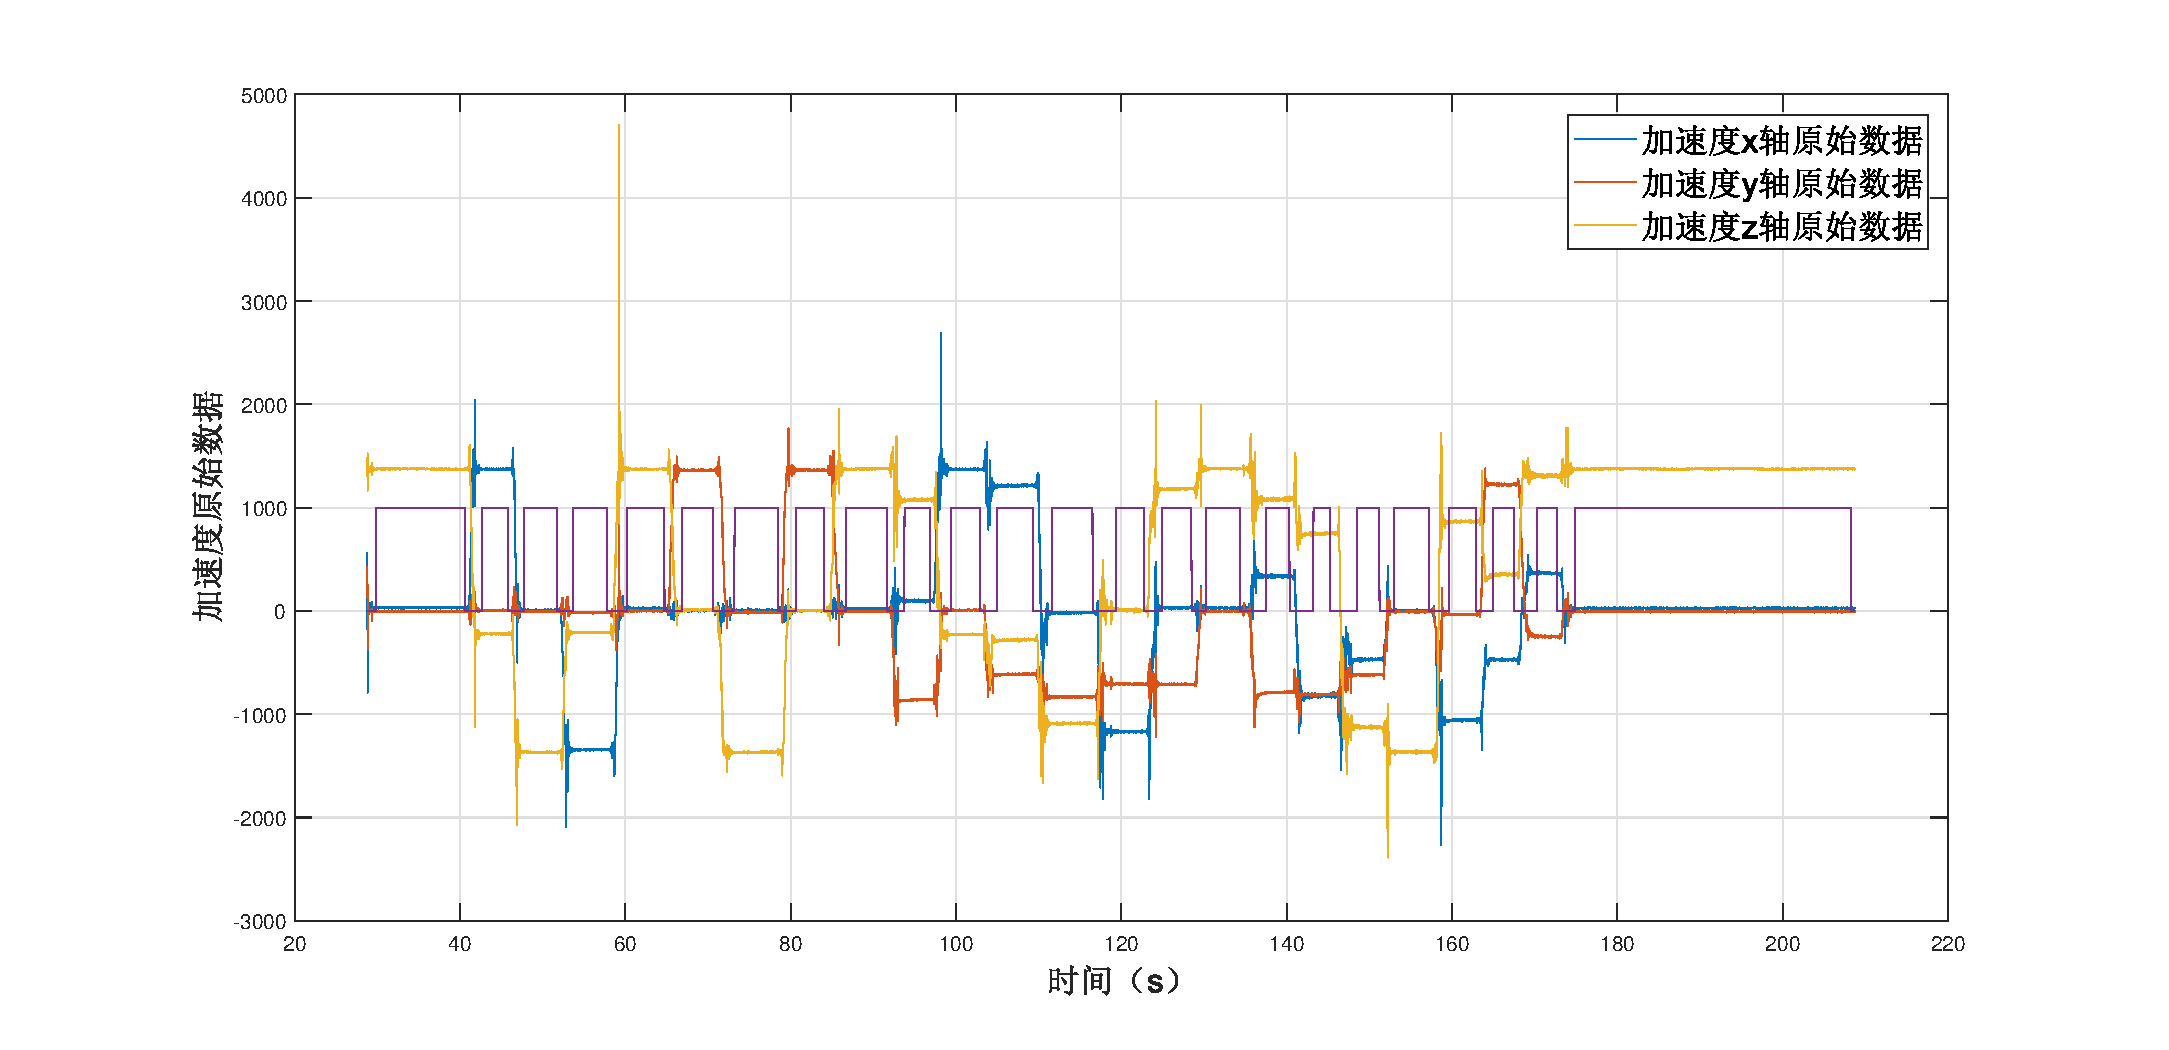
\includegraphics[width=1.0\textwidth]{staticdetect3.eps}
	\bicaption{静态区间分割效果}{Static interval extraction result}
	\label{fig:staticdetect}
\end{figure}
通过观察\autoref{fig:staticdetect}中的加速度曲线是否变化可判断出当前飞控板的状态是运动还是静止,可直接看出区间分割的效果。
从\autoref{fig:staticdetect}中可得出以下结论:

(1)紫色高电平区间内为静态区间。

(2)静态检测器效果很好,区间不会包含运动部分。

接着,按照本文提出的算法对加速度计和陀螺仪进行校准。
一共需要求出12个参数。
校准实验结果如\autoref{IMUparameters}所示。
\begin{table}[H]
	\bicaption{IMU参数}{IMU parameters}
	\label{IMUparameters}
	\begin{tabular}{ccc}
		\toprule
		参数 & 加速度计 & 陀螺仪 \\
		\midrule
		$\beta_{yz}$ & -0.0039 & 0.0034\\
		$\beta_{zy}$ & 0.0081 & 0.0038\\
		$\beta_{xz}$ & 0.0002 & -0.0013\\
		$\beta_{zx}$ & -0.0037 & 0.0040\\
		$\beta_{xy}$ & -0.0072 & -0.0078\\
		$\beta_{yx}$ & 0.0047 & 0.0023\\
		$s_x$ & 0.9921 & 1.0006\\
		$s_y$ & 0.9963 & 1.0003\\
		$s_z$ & 0.9959 & 0.9993\\
		$b_x$ & 14.7897 & 2.0444\\
		$b_y$ & -7.4082 & -2.6646\\
		$b_z$ & 3.0406 & 0.5780\\
		\bottomrule
	\end{tabular}
\end{table}
在得到IMU校准参数后,对校准效果进行评估。
%对于加速度计,观察校准前和校准后加速度的输出。
分别绘制校准前和校准后的加速度计输出的重力模长对比曲线如\autoref{fig:acccalib}所示。
\begin{figure}[H]
	\centering
	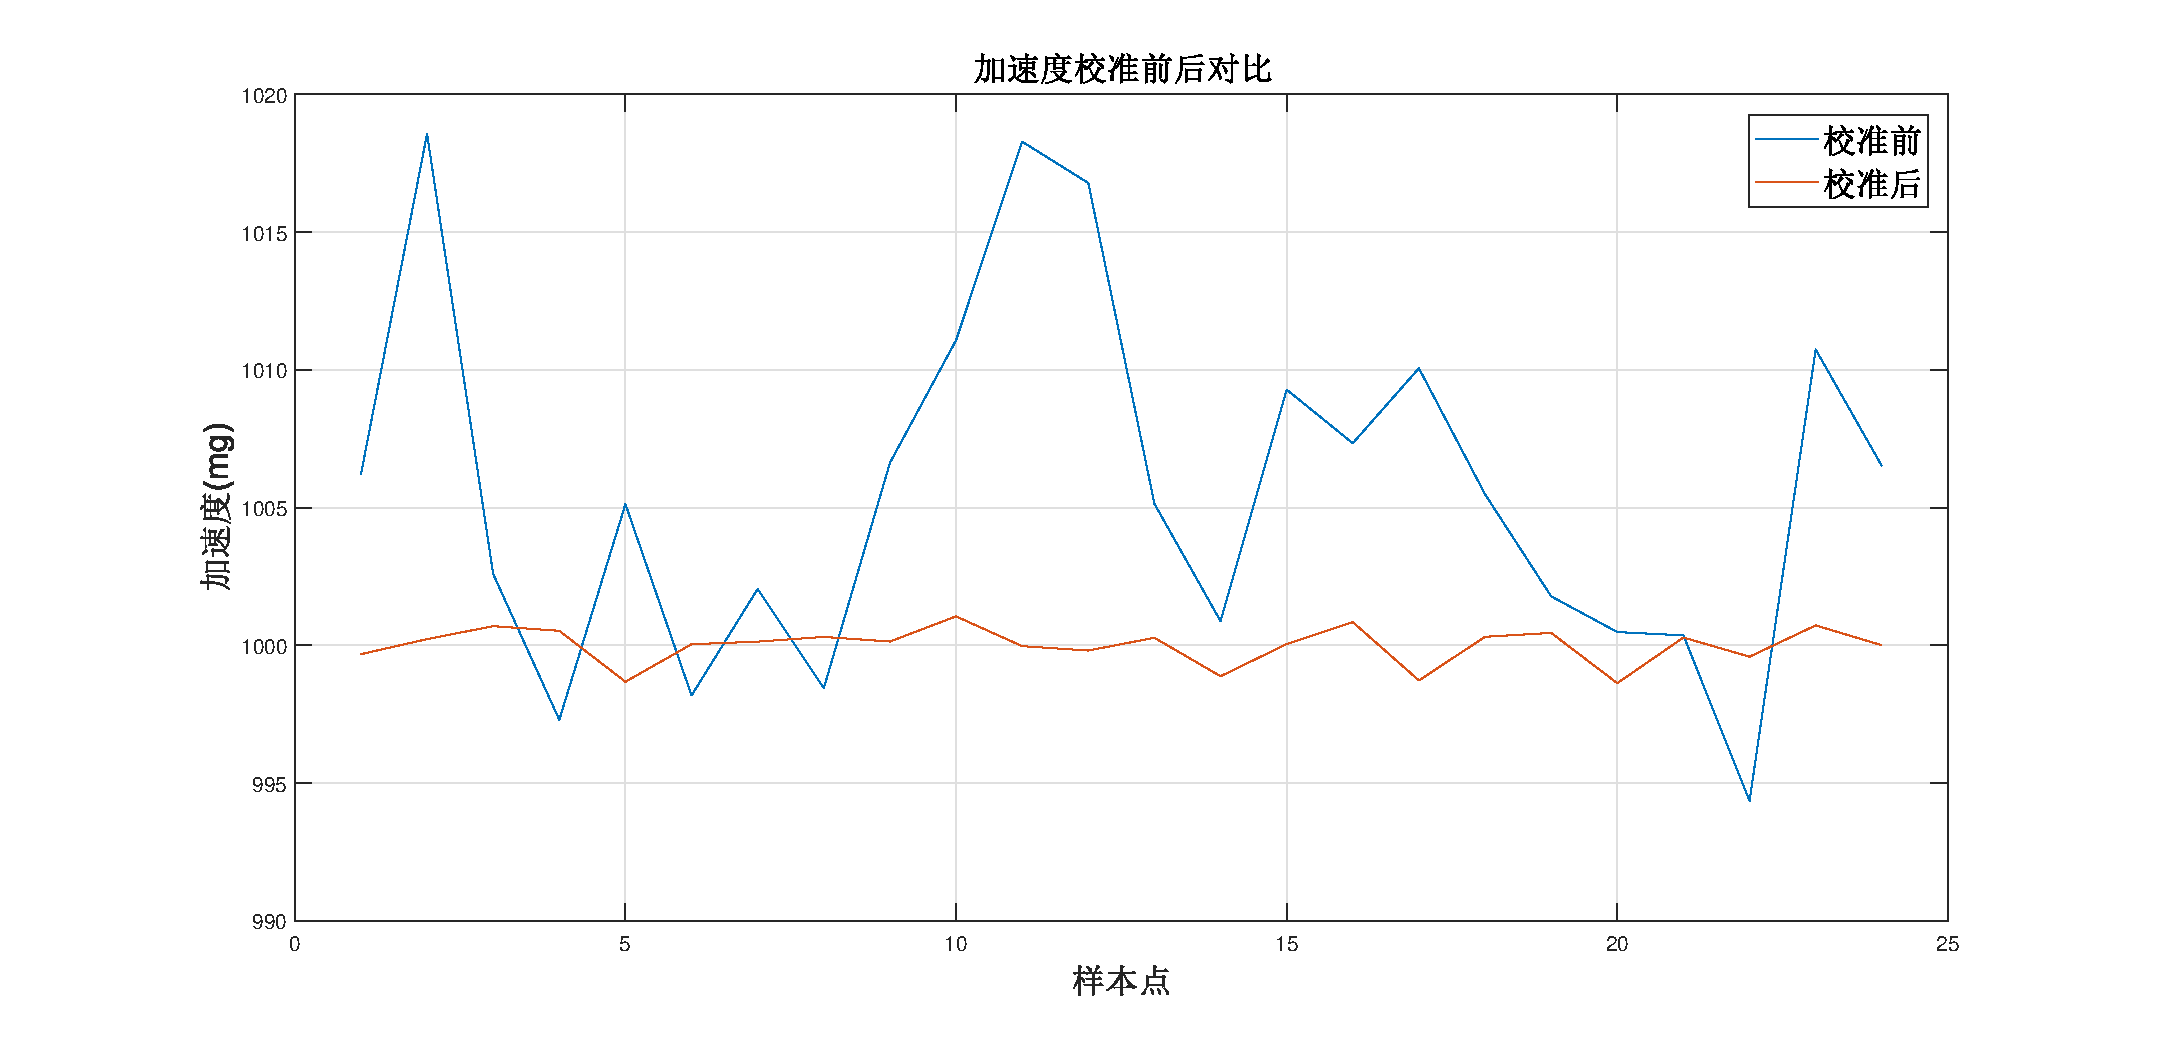
\includegraphics[width=1.0\textwidth]{acccalib1.eps}
	\bicaption{加速度校准前后对比}{Acceleration calibration before and after comparison}
	\label{fig:acccalib}
\end{figure}
对于加速度计,重力的模长作为真值。
通过比对每一个静态区校准前和校准后加速度计输出的模长与重力模长的误差可评估校准性能。
从\autoref{fig:acccalib}看出有24个静止点,校准前的加速度模长波动超过20mg,校准后的加速度模长波动小于2mg。加速度计的校准误差如\autoref{acccaliberr}所示。
\begin{table}[H]
	\bicaption{加速度计校准误差}{Accelerometer calibration error}
	\label{acccaliberr}
	\begin{tabular}{ccc}
		\toprule
		状态 & 平均误差($m/s^2$) & 最大误差($m/s^2$) \\
		\midrule
		校准前 & 0.0641 & 0.1819 \\
		校准后 & 0.0049 & 0.0135 \\
		\bottomrule
	\end{tabular}
\end{table}
其中,平均误差是指加速度计输出的数据模长与重力模长的差的平均值,最大误差是指所有加速度计输出的数据模长中与重力模长的差的最大值。

从\autoref{fig:acccalib}和\autoref{acccaliberr}可得出以下结论:

(1)校准后的加速度静止状态下更接近于重力。

(2)校准后的误差$<0.005m/s^2$,传感器误差可以满足实际使用要求。

%对于陀螺仪,使用角速度积分的姿态评估校准性能。
%校准后的加速度计的输出作为真值。
对于陀螺仪,进行了两个评估实验:
(1)分段区间积分姿态对比;
(2)全过程积分姿态对比。
%对于第一个实验,在每一个运动区间,使用\autoref{eq:rk4}通过对起点到终点的角速度积分可计算出姿态四元数,然后转换到欧拉角。
%首先绘制分段区间积分姿态对比曲线如\autoref{fig:piece}所示。
%校准后的加速度计可计算出欧拉角(姿态)作为真值。
%实验结果如\autoref{fig:piece}和\autoref{fig:full}所示。
%对于每一个运动区间,使用\autoref{eq:rk4}通过对起点到终点的角速度积分可计算出姿态四元数,然后转换到欧拉角,这样比对校准前和校准后欧拉角与真值的误差可评估校准性能。
%另一方面,可以对采样过程中的角速度数据进行全段积分,对比校准前和校准后的姿态曲线与真值接近程度可评估校准性能。
%实验结果如\autoref{fig:piece}和\autoref{fig:full}所示。
\begin{figure}[H]
	\centering
	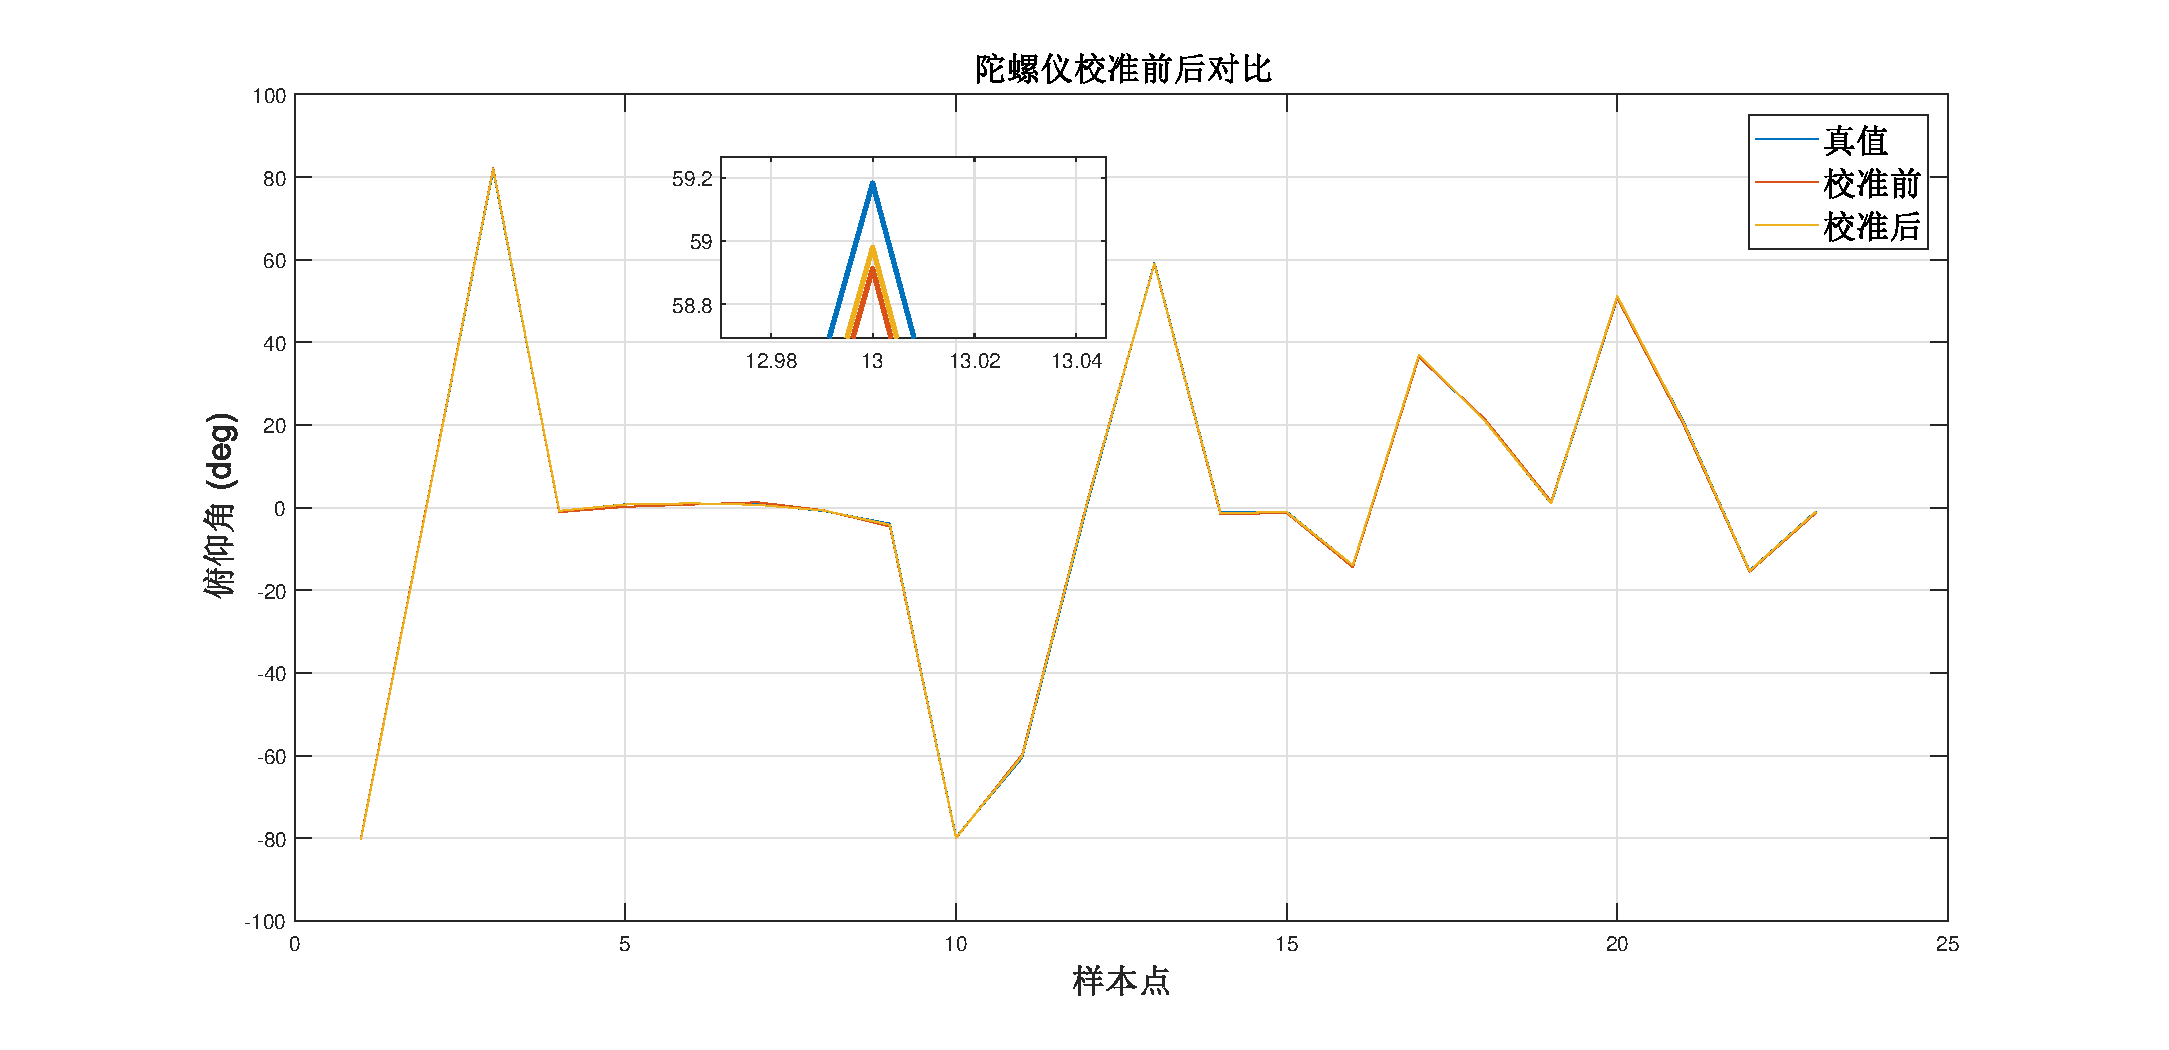
\includegraphics[width=1.0\textwidth]{piece1.eps}
	\bicaption{分段姿态积分对比}{Piece attitude integral comparison}
	\label{fig:piece}
\end{figure}
对于每一个运动区间,使用\autoref{eq:rk4}对起点到终点的角速度积分可计算出姿态四元数,然后转换到欧拉角。分段区间积分姿态对比曲线如\autoref{fig:piece}所示。
通过比对每一个样本点校准前和校准后欧拉角与真值的误差可评估校准性能。
结果表明,使用校准后计算的俯仰角比使用校准前更加接近真值。
\begin{figure}[H]
	\centering
	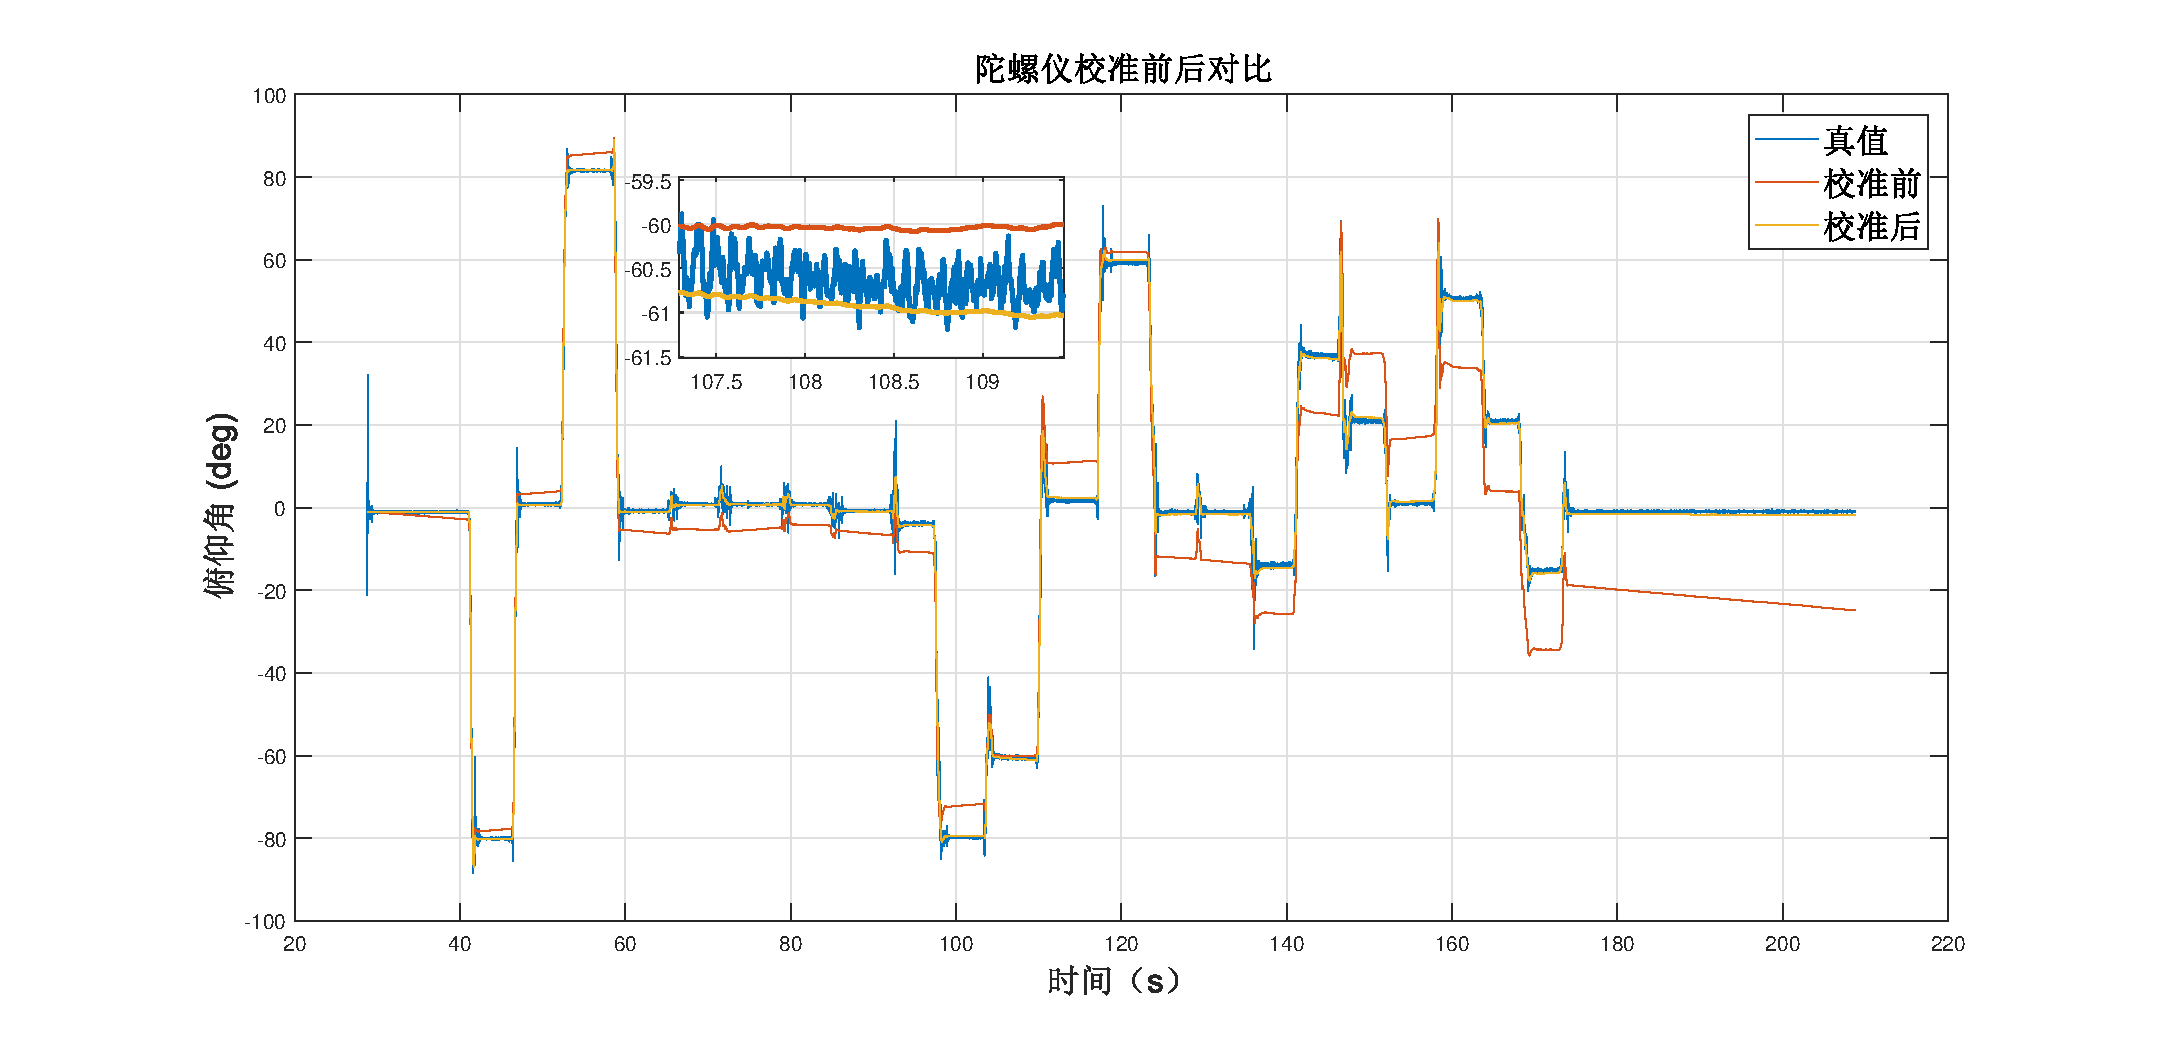
\includegraphics[width=1.0\textwidth]{full1.eps}
	\bicaption{全程姿态积分对比}{Overall attitude integral comparison}
	\label{fig:full}
\end{figure}
%接着绘制分段区间积分姿态对比曲线如\autoref{fig:piece}所示。
接着对采样过程中的角速度数据进行全段积分,对比校准前和校准后的姿态曲线与真值接近程度可评估校准性能。
如\autoref{fig:full}所示,使用校准后的陀螺仪计算的俯仰角曲线比使用校准前的陀螺仪计算的俯仰角曲线更加接近真值。
陀螺仪校准误差如\autoref{gyrocaliberr}所示。
\begin{table}[H]
	\bicaption{陀螺仪校准误差}{Gyroscope calibration error}
	\label{gyrocaliberr}
	\begin{tabular}{ccc}
		\toprule
		状态 & 平均误差(度) & 最大误差(度) \\
		\midrule
		校准前 & 1.4431 & 1.5965 \\
		校准后 & 0.1255 & 0.8970 \\
		\bottomrule
	\end{tabular}
\end{table}
其中,平均误差是陀螺仪短期积分的姿态与加速度计计算的姿态的差的平均值,最大误差是指所有陀螺仪短期积分的姿态与加速度计计算的姿态的差的最大值。

从\autoref{fig:piece}、\autoref{fig:full}以及\autoref{gyrocaliberr}可得出以下结论:

(1)不管是分段积分还是全段积分,使用校准后的陀螺仪积分出来姿态更接近与真值。
在全段积分中,由于陀螺仪零偏的存在,使用校准前的陀螺仪积分出来姿态存在漂移现象。

(2)校准后的误差$<0.13$度,传感器误差可以满足实际使用要求。
%\begin{table}[htbp]
%	\bicaption{IMU参数}{IMU parameters}
%	\label{IMUparameters}
%	\begin{tabular}{ccccccccccccc}
	%		\toprule
	%		传感器 & $\beta_{yz}$ & $\beta_{zy}$ & $\beta_{xz}$ & $\beta_{zx}$ & $\beta_{xy}$ & $\beta_{yx}$ & $s_x$ & $s_y$ & $s_z$ & $b_x$ & $b_y$ & $b_z$\\
	%		\midrule
	%		加速度计 & -0.0039 & 0.0081 & 0.0002 & -0.0037 & -0.0072 & 0.0047 & 0.9921 & 0.9963 & 0.9959 & 14.7897 & -7.4082 & 3.0406\\
	%		陀螺仪 & 0.0081 & 0.0038\\
	%		\bottomrule
	%	\end{tabular}
%\end{table}

\gdutsubsection{算法对比}{Algorithm comparison}
通过校准性能评估实验可以得出本文的校准算法是达到要求的。
%接下来说明本文算法改进的地方。
对于文献\parencite{tedaldi2014robust}提出的算法,本实验测试了其阈值计算的结果如\autoref{fig:res}所示。
\begin{figure}[H]
	\centering
	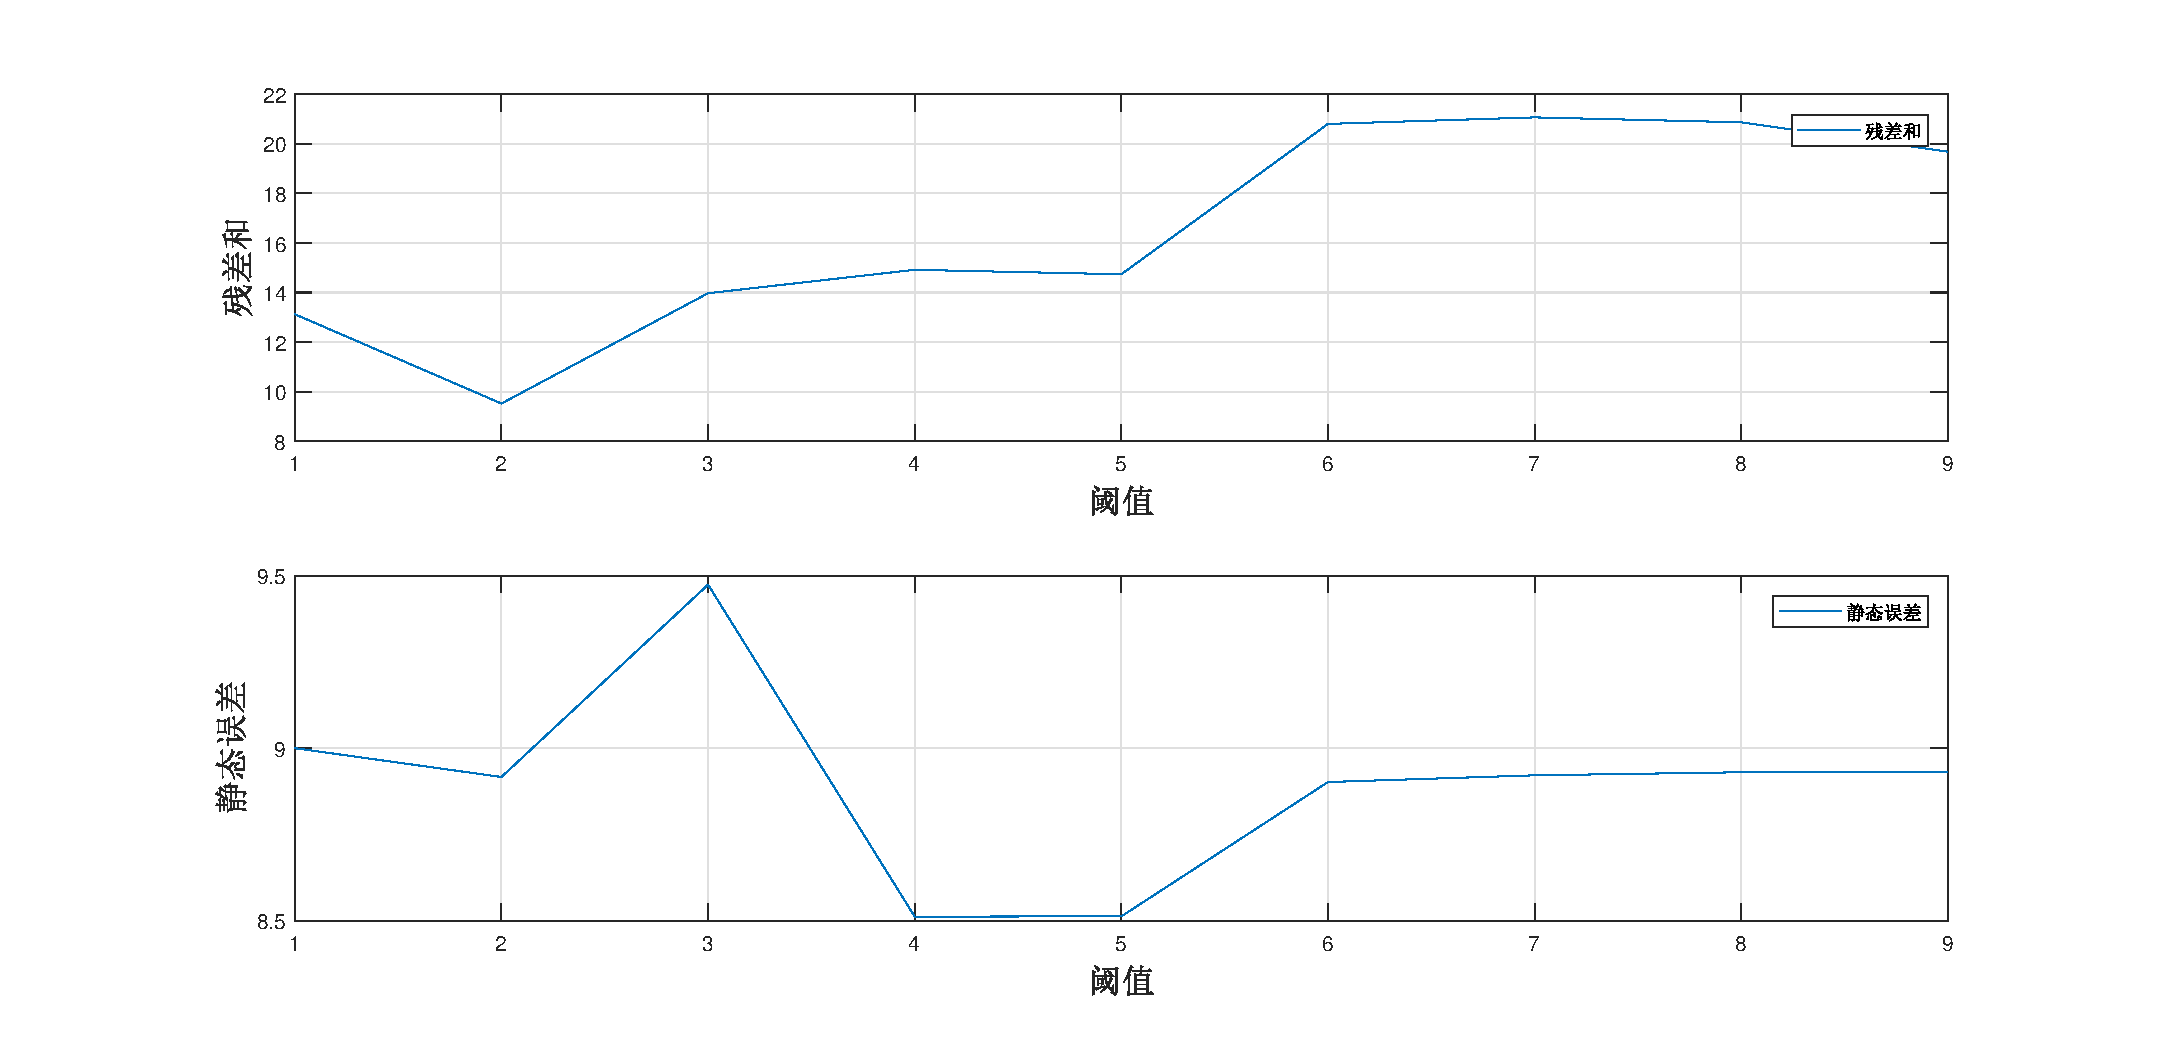
\includegraphics[width=1.0\textwidth]{res2.eps}
	\bicaption{阈值计算对比}{Threshold calculation comparison}
	\label{fig:res}
\end{figure}

Tedaldi计算最优阈值的原则是残差和最小,程序会选择残差和最小对应的阈值作为最优阈值。
本文测试了当样本数为16时Tedaldi和本文算法的结果。
从\autoref{fig:res}可得出以下结论:

(1)残差在$k=2$时是最小的,在$k=7$之后随着样本的增加逐渐减少。

(2)根据残差变化规律,其和样本数以及整数$k$有关,在样本较小时残差会较小,样本较多时才能达到一个最优的选取效果。

(3)由图可以得出最优阈值$k=2$的结论,但实际上$k=2$得出的区间是很少的,反而会导致校准效果不佳。
基于以上分析,使用误差计算阈值的方法是更合理的。
本文给出Tedaldi的方法和本文的方法的误差分析,如\autoref{Algorithmerrorcomparison}所示。
本文提出的算法的误差比Tedaldi算法的误差要小,因此本文的IMU校准算法要优于Tedaldi的方法。
%接下来给出两个算法的误差分析。
\begin{table}[H]
	\bicaption{算法误差对比}{Algorithm error comparison}
	\label{Algorithmerrorcomparison}
	\begin{tabular}{ccc}
		\toprule
		算法 & 平均误差($m/s^2$) & 最大误差($m/s^2$) \\
		\midrule
		Tedaldi & 0.0078 & 0.0820 \\
		本文 & 0.0049 & 0.0135 \\
		\bottomrule
	\end{tabular}
\end{table}
%从\autoref{Algorithmerrorcomparison}可得出以下结论:本文的IMU校准算法要优于Tedaldi的方法。

\gdutsection{总结与讨论}{Summary and discussion}
本章设计了IMU校准算法。
针对分割阈值计算存在非最优的情况导致加速度计校准效果不佳的问题,提出了一种检测阈值最优计算算法,解决了加速度计校准结果不准确的问题。
和Tedaldi的算法相比,本文提出的算法修改了阈值计算的步骤。
由于本算法需要对每个阈值都进行误差计算,所以会增加算法的运行时间。
考虑到校准不是实时的,这部分时间是可以接受的,但本文的算法的校准精度更高。

\gdutchapter{抗干扰多源信息融合方法}{Anti-disturbance multi-source information fusion method}
基于第二章描述的IMU校准方法,本章将使用IMU作为主要传感器,设计一种适用于多旋翼飞行器的状态估计算法。
为保证多旋翼飞行器在恶劣环境中的作业的可靠性和稳定性,需要多传感器信息融合方法和传感器扰动抑制处理来获取更好的状态信息。
本文设计的多旋翼飞行器搭载的传感器包括IMU(陀螺仪+加速度计)、磁力计、GNSS以及气压计,采用的状态估计框架如\autoref{fig:stateestimation}所示。
从\autoref{fig:stateestimation}可以看出传感器系统具有多延时和多频率的特性。
本章将对这些特性不同的传感器通过融合算法实现优势互补,保证高精度的状态输出。
%本课题感兴趣的是在飞行器平台上运行的状态估计算法,这种应用场景对于传感器融合有更严格更复杂的要求。
%在这些环境中,依赖单一现有成果的算法是不可行的。
%本文注意到,这个课题已经有很多的研究成果\cite{mahony2008nonlinear,hua2010attitude,khosravian2016state}。
%本文的工作与现有成果之间的主要区别在于,本文的方法在前人工作的基础上,提出了新的框架,具有很强的鲁棒性,能确保该系统能够在大震动、高机动环境、磁场干扰环境中稳健运行。
%本文给出了各种环境下的实验结果,要求系统在一段较长的时间内无故障运行。
\begin{figure}[H]
	\centering
	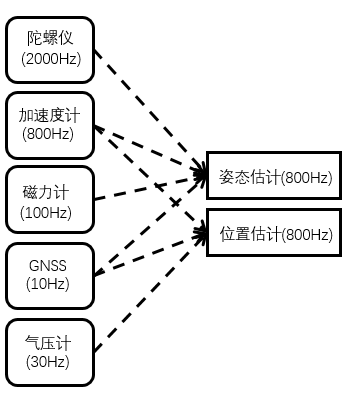
\includegraphics[width=0.55\textwidth]{屏幕截图 2022-06-08 110601.png}
	\bicaption{状态估计框架图}{Diagram of state estimation}
	\label{fig:stateestimation}
\end{figure} 
%本章将重点讨论系统中使用的状态估计方法。
%\autoref{fig:stateestimation}展示了本文状态估计的框架。
%本章主要针对多旋翼无人机的导航信息融合和容错方法开展研究。
%本文注意到,自主飞行需要仔细地集成其他重要模块,如控制、校准等。
%这些模块的讨论放到后面两章。
%这些模块作为通用模块,以支持整个系统的运行。
\gdutsection{传统状态估计方法分析}{Analysis of traditional state estimation methods}
%将状态估计问题用数学语言表述之后,本节将讨论具体的算法实现,分析各种算法的优劣以及目前存在的问题,以引出本文的设计。

\gdutsubsection{矢量观测}{Vector observations}
%Note 总结矢量观测
%位置信息可以从位置传感器拿到,而姿态信息的计算是相对而言比较困难的。
矢量观测是测量一些在世界坐标系内已知的矢量,这些矢量在机体坐标系中的测量值包含了IMU自身的姿态信息。
因此,基于矢量观测的方法可以测量姿态。
例如,用IMU中的加速度计测量重力方向,用磁力计测量磁场方向等。
上述例子都是将方向测量转化为姿态测量,这一问题在姿态估计的文献中被称为Wahba问题(Wahba's Problem)\cite{wahba1965least}。
Shuster于1979年在文献\parencite{shuster1981three}中提出的QUEST(QUaternion ESTimator)算法用于解决Wahba问题。
这些算法需要在计算时间和精度之间进行权衡,例如,迭代的次数必须提前定义。
此外,矢量观测的本质是代数解法,其主要缺点是没有记忆特性,即过去测量的状态所包含的信息没有被保存下来。

\gdutsubsection{观测器}{Observer}
观测器算法是作为替代代数方法的解决方案被提出的,在更多场合中被称作滤波器。
观测器将矢量测量与运动学方程结合起来,当矢量测量值有噪声时,通常首选观测器算法。
在这类算法中,非线性观测器是一类十分有价值的方法,因为它们通常具有更强的稳定性和鲁棒性,非常容易调参和实现。
Mahony等人提出的非线性显式互补滤波器是一个被广泛运用的方法\cite{mahony2008nonlinear}。
后续有相当多的工作在非线性显式互补滤波器上的改进\cite{hua2010attitude,khosravian2016state}。
本文发现,基于观测器的方法可以简单地通过使用多个测量模型融合多个传感器。
然而,标准的观测器方法只保留最新的状态量。
因此,对于多频率多延时传感器的融合则更为复杂。
为了解决这一问题,本研究提出一种新的融合框架以处理多源信息融合困难的问题。

\gdutsubsection{显式互补滤波器}{Explicit complementary filter}
在无人机的姿态估计中,一个十分流行的算法是Mahony等人提出的在SO(3)群上的互补滤波器\cite{mahony2008nonlinear}。
接下来简单地分析以下显式互补滤波器是如何工作的。

姿态估计的目标是为估计量$\hat{R}(t)\in SO(3)$提供一组动力学方程来使得误差旋转矩阵$\widetilde{R}(t)\rightarrow I_3$。
文献\parencite{mahony2008nonlinear}所提出的观测器方程直接作为一个运动学系统用于姿态估计。此观测器运动学包括基于测量的预测项和由误差导出的修正项。
记$\hat{R}$表示对飞行器姿态$R$的估计,观测器的一般形式是
\begin{equation}\label{eq:passivefilter}
	\dot{\hat{R}}=\hat{R}(\omega_{\times}+k_P \mathbb{P}_a(\widetilde{R}))
\end{equation}
其中,$k_P>0$。观测器框架如\autoref{fig:DiagramECF}所示。
\begin{figure}[htbp]
	\centering
	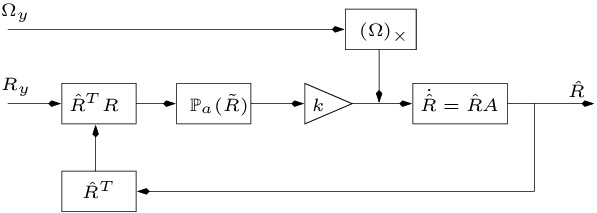
\includegraphics[width=1.0\textwidth]{Block-diagram-of-the-simplified-form-of-the-passive-complementary-filter.png}
	\bicaption{显式互补滤波框架图}{Block diagram of explicit complementary filter}
	\label{fig:DiagramECF}
\end{figure}
对于$\mathbb{P}_a(\widetilde{R})$,可以使用欧拉角相减,DCM或四元数相乘来获取姿态的误差。但是这样的方法都有一个缺点,即需要通过加速度计和磁力计的测量计算出一组姿态。
虽然常用的方法比较成熟,但也有一些问题,比如欧拉角法存在奇异点(如在俯仰角90度时),DCM和四元数的TRIAD或QUEST等方法又需要额外的计算。
显式互补滤波器的突出贡献之一就是直接利用加速度计和磁力计的测量值,利用和惯性空间向量的叉乘,简单地就获得了姿态的误差。
如下观测器是\vspace{1ex}显式互补滤波器的标准形式
\begin{gather}\label{eq:Explicitfilter}
		\dot{\hat{R}} =\hat{R}((\omega^y - \hat{b})_{\times}+k_P (\omega_{mes})_{\times})\\
		\dot{\hat{b}} =-k_I \omega_{mes}\\
		\omega_{mes} \coloneqq \sum_{n=1}^{n} k_i v_i \times \hat{v}_i	
\end{gather}
其中$k_P$,$k_I$,$k_i$是任意非负的观测器增益。
$v_i$是可用的矢量测量。
注意到姿态$\hat{R}$是整个观测器的输出。
在文献\parencite{mahony2008nonlinear}中对观测器(\autoref{eq:Explicitfilter})进行了广泛的研究,表明姿态和零偏在理论和实验上能做到指数收敛。
该滤波器具有互补的特性,利用陀螺仪信号的高频部分和磁力计、加速度计的低频部分\cite{mahony2008nonlinear}。
与这些信号相关联的截止频率由增益$k_P$,$k_I$,$k_i$决定。
用于表示旋转的单位四元数在代码实现中具有较高的效率,是实现SO(3)\vspace{1ex}群运算的常用方法。
上述观测器的四元数表示如下
\begin{gather}\label{eq:quatfilter}
		\dot{\hat{q}}=\frac{1}{2} \hat{q} \otimes \mathbf{p}(\omega_y - \hat{b} + k_P \omega_{mes})\\
		\dot{\hat{b}}=-k_I \omega_{mes}\\
		\omega_{mes} \coloneqq \sum_{n=1}^{n} k_i v_i \times \hat{v}_i	
\end{gather}

\gdutsection{抗干扰多源信息融合算法设计}{Design of anti-jamming multi-source information fusion algorithm}
本节描述了一种融合来自多频率多延时传感器信息的方法,以提高系统在各种环境中的鲁棒性。
这项工作的主要目标是开发一种模块化和可扩展的方法来集成来自多个传感器的测量值,为稳定飞行提供平滑准确的实时状态估计。
本文第一个关键贡献,也是本文工作的核心,是一种基于\parencite{mahony2008nonlinear}的原则性方法,通过预测-修正-延时框架来融合所有传感器的测量值。
第二个重要的贡献是本文提出的观测器公式,它的更新步骤避免扰动对状态影响的耦合以及异常处理的困难。
%最后,本文使用实验平台(\autoref{fig:platform})测试了结果,以说明本文的融合框架在飞行中的鲁棒性。
%算法流程如\autoref{fig:Flowchartoffusionalgorithm}所示。
%note:说明图片
%这里只大致概括了对信息处理的一个流程。
%在这个流程里,最重要的信息是陀螺仪输出的角速度信息以及加速度计输出的加速度信息。
%可以看到即便其他传感器出现故障或者丢失信息的情况,算法的信息流依然是完整的。
\gdutsubsection{融合算法流程}{Fusion algorithm flow}
%IMU是传感器系统中最核心的传感器,其输出的惯性数据具有高频率的特性。
%因此,算法的核心是通过IMU预测飞行器的状态。
%其中,使用陀螺仪的角速度预测更新姿态,使用加速度计的运动加速度分量
%本节介绍融合算法的总流程。
融合算法的流程可以简单分解为预测和修正两个核心步骤。
首先通过刚体运动学方程可预测飞行器的状态,然后通过测量信息修正状态。
其中,IMU是传感器系统中最核心的传感器,其输出的惯性数据具有高频特性。
因此,融合算法的核心是通过IMU输出的惯性信息预测飞行器的状态。
其中,使用陀螺仪的角速度预测更新姿态,使用加速度预测更新速度和位置。
当速度或位置传感器更新时,使用速度或位置信息修正位置,同时可求出运动加速度补偿姿态修正。
本文的融合算法总流程如\autoref{fig:Flowchartoffusionalgorithm}所示。
\begin{figure}[H]
	\centering
	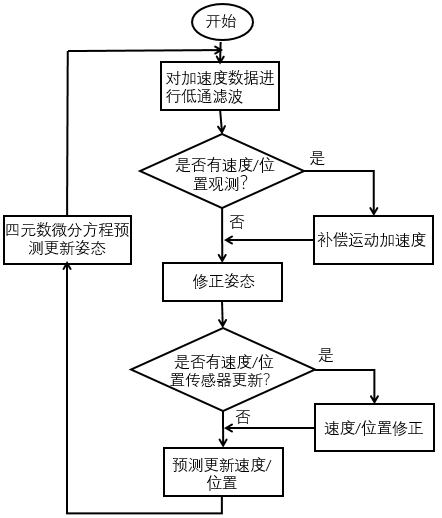
\includegraphics[width=0.68\textwidth]{屏幕截图 2022-06-08 113324.png}
	\bicaption{融合算法流程图}{Flow chart of fusion algorithm}
	\label{fig:Flowchartoffusionalgorithm}
\end{figure}

\gdutsubsection{预测-修正-延时融合框架}{Prediction-correction-delay fusion framework}
针对飞行器应用开发从业人员,本课题希望设计一个模块化、容易扩展的传感器融合观测器。
这意味着当需要增加或删除传感器时需要数学推导和编程的工作量应该是最小的。
但是前人的工作只提供了一般的算法框架,或者是针对特定传感器的优化算法,很少工作能兼容多个传感器并且能随意增加和删除传感器。
因此,从数据融合的角度,本课题提出了预测-修正-延时融合框架。
%如\autoref{fig:Delayedmeasurementupdate}所示。

当需要融合多个测量值时,传感器的采样频率是不统一的,即每种传感器测量值更新的频率都有可能不一样。
此外,由于传感器内部处理的延时,所有的测量值都是滞后于当前的状态的。

对于多采样频率问题,可以将更新和预测都放在预测的任务中处理,因为基于IMU的预测更新总是最快的,这样可以保证对每个用于修正的传感器数据都能及时使用。

对于延时问题,可使用观测器-预测器方法\cite{khosravian2014velocity}。
将状态值、测量值存储在队列中,队列的顶部对应于最旧的状态值。
在本文的程序软件上,预先定义了最大允许的传感器延迟$t_d$为100ms。
如果更新的测量值相对于当前状态(观测器输出的)的延时大于$t_d$,这个测量值就直接丢弃。
对于姿态、位置、速度都有其对应的队列,状态队列长度是所有传感器的最大延时$t_d^{max}$,传感器可针对需求生成自己的队列(比如GPS)。
在观测器中,总是利用最新的IMU测量值来向前更新状态。
记$x_i$是估计器输出的状态量,$z_i$是传感器的测量值,具体的处理机制如\autoref{fig:Delayedmeasurementupdate}所示。
%为了方便说明,将所有的状态都计为$x_i$,测量值都计为$z_i$。
\begin{figure}[htbp]
	\centering
	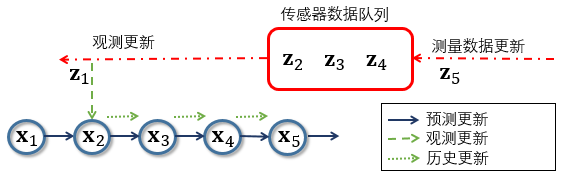
\includegraphics[width=1.0\textwidth]{屏幕截图 2022-06-08 115635.png}
	\bicaption{预测-修正-延时融合框架}{Prediction-correction-delay fusion framework}
	\label{fig:Delayedmeasurementupdate}
\end{figure} 

$z_1$作为最旧的状态,首先输入到观测器上。
$z_2$、$z_3$、$z_4$临时存储在队列中。
根据传感器的延时$z_1$用于修正$x_2$的状态,然后向前更新历史状态。
最新的状态$x_5$则通过最新的IMU数据进行预测更新。

这样,可以方便的增加或减少传感器,在程序中即增加或减少队列,同时可以为每个传感器设置延时,进行时间同步。

\gdutsubsection{状态预测更新}{State propagation}
由于陀螺仪的采样频率和加速度计的采样频率不一致,将姿态预测和姿态修正分离,只要陀螺仪数据更新,就根据\autoref{eq:quatkinematics}使用角速度数据进行积分。
\begin{equation}\label{eq:quatint}
	\dot{q}(k)=\frac{1}{2} q \otimes \mathbf{p}(\omega_y(k))
\end{equation}
\vspace{1ex}只要加速度数据更新,就使用加速度数据进行积分。其中$\Delta t$是步长。
\begin{gather}\label{eq:pvpredict}
		a^w(k) = \hat{R}_b^w a^b(k) - g e_3\\
		v(k) = v(k-1) + a^w(k) \Delta t\\
		p(k) = p(k-1) + v(k) \Delta t 
\end{gather}

\gdutsubsection{运动加速度延时补偿修正}{Motion acceleration delay compensation correction}
%对于加速度计来说,某些构型的飞行器机身可产生10个重力加速度大小的震动,加速度计对震动非常敏感,飞行过程中姿态的真实信息被震动加速度淹没了。
%针对震动噪声的问题,一般的解决方案是对加速度的数据进行一个低截止频率的低通滤波。
对于姿态来说,运动加速度是作为加速度计的扰动输入进修正项影响姿态精度。
针对运动加速度补偿问题,一般的解决方案是使用GPS的线速度进行补偿,但是GPS速度存在延时问题,还需要对历史状态处理。
文献\parencite{khosravian2014velocity}使用观测器-预测器方法对历史状态处理,在机体系下求出历史误差,但并没有对历史状态进行修正。
由于每个历史状态的机体系都是不一样的,不同坐标系的向量无法进行运算,所以使用机体系下的误差对历史状态修正在实际应用中并不准确。
因此,本文提出的算法对修正量进行修改,在世界系求姿态误差,然后对历史状态进行修正。
此外,由GPS差分的运动加速度和IMU的更新频率不一致,进一步用线性插值计算运动加速度作补偿。
\vspace{1ex}设计如下观测器:
\begin{gather}\label{eq:myrpcorrection}
		\Delta a = \frac{v - v_{last}}{\Delta t}\\
		a_m (k-d) = a_{last} + \frac{k-d}{k-k_{last}} \Delta a\\
		a_{ref} (k-d) = a_m (k-d) + g e_3\\
		\sigma = k_a \hat{R}(k-d) a(k-d) \times a_{ref}(k-d)\\
		q_{correction}^{RP} = \mathbf{p}(\sigma)\\
		\hat{q}(k-n) = q_{correction}^{RP} \otimes \hat{q}(k-n)
\end{gather}
其中,$a_m (k-d)$为$k-d$时刻通过插值计算的运动加速度,$\hat{R}(k-d)$为$k-d$时刻的姿态,$\sigma$为$k-d$时刻的修正量。
使用$k-d$时刻的误差修正当前状态。
$q_{correction}^{RP}$是修正四元数,只修正横滚角$\phi$、俯仰角$\theta$分量。
取$n=0,1,...,d$修正$k-d$时刻到$k$时刻的历史状态。

可以注意到,标准显式互补滤波器(\autoref{eq:quatfilter})相比,本文的观测器继承了其使用叉乘计算误差的特性,对运动加速度以及延时的影响进行了优化处理。

\gdutsubsection{偏航解耦修正}{Yaw decoupling correction}
磁场干扰和零偏会影响横滚角$\phi$和俯仰角$\theta$的估计。
在实际应用中,特别是在使用电机作为执行器的小型飞行器中,较大的磁场干扰几乎是不可避免的,导致磁力计测量值$m_y$和$R^T m^w$之间存在较大的时变误差。
这不仅会导致偏航角的估计误差很大,而且还会导致横滚角和俯仰角估计产生误差。
由于横滚角,俯仰角和偏航角估计的动力学方程是高度耦合的,这意味着偏航角的估计会较大地影响着横滚角和俯仰角的估计。

解耦的关键在于能否在计算上区分开来,由于将磁场向量转换到机体系上做修正,并且磁场向量本身包括x轴,y轴分量,这些分量会影响到横滚角$\phi$、俯仰角$\theta$分量。
实际上,完全可以将横滚角$\phi$、俯仰角$\theta$分量的四元数和偏航角$\psi$分量的四元数分离开,当获取到磁力计数据时,只用磁力计修正偏航分量的四元数,然后生成一个完整的姿态。

注意到在姿态修正过程中横滚角$\phi$、俯仰角$\theta$分量和偏航角$\psi$分量的明显区别,首先将姿态划分为横滚角$\phi$、俯仰角$\theta$分量四元数和偏航角$\psi$分量四元数:\vspace{1ex}
\[
q^{RP} = 
\begin{bmatrix}
	q_w^{RP} \\
	q_x^{RP} \\
	q_y^{RP} \\
	q_z^{RP}
\end{bmatrix},
\hspace{1em}
q^{Y} = 
\begin{bmatrix}
	q_w^{Y} \\
	q_x^{Y} \\
	q_y^{Y} \\
	q_z^{Y}
\end{bmatrix}
\]
通过对姿态四元数分解,其关系为:
\begin{equation}\label{eq:decompose}
	q = q^{Y} \otimes q^{RP}	
\end{equation}
由此可以看出,对完整的姿态四元数修正实际上是不必要的,偏航分量只对应于$q^{Y}$。
可以通过磁力计计算的偏航角只修正$q^{Y}$,然后通过\autoref{eq:decompose}叠加到完整的姿态四元数上。
由于横滚角$\phi$、俯仰角$\theta$分量只存在于四元数$q^{RP}$,因此避免了磁场干扰对横滚角$\phi$、俯仰角$\theta$的影响。
由于欧拉角定义的旋转顺序是ZYX,偏航分量四元数的定义如\autoref{eq:yawquat}所示:
\begin{equation}\label{eq:yawquat}
	q^{Y} = 
	\begin{bmatrix}
		cos(\frac{\hat{\psi}}{2}) \\
		0 \\
		0 \\
		sin(\frac{\hat{\psi}}{2})
	\end{bmatrix}	
\end{equation}
偏航修正方式可以按照线性互补的方法进行修正:
\begin{equation}
	\hat{\psi} = k_{\psi} (\psi_{mag} - \hat{\psi}) 	
\end{equation}
其中,$k_{\psi} > 0$,$\hat{\psi}$为修正后的偏航角,$\psi_{mag}$为磁力计测量的偏航角。

对磁力计的延时处理,设计如下观测器:\vspace{1ex}
\begin{gather}\label{eq:myyawcorrection}
		\sigma = k_{\psi} (\psi_{mag}(k-d) - \hat{\psi}(k-d)) \\
		q_{correction}^{Y} = \begin{bmatrix}
			cos(\frac{\sigma}{2}) \\
			0 \\
			0 \\
			sin(\frac{\sigma}{2})
		\end{bmatrix}\\
		\hat{q}(k-n) = q_{correction}^{\psi} \otimes \hat{q}(k-n)
\end{gather}
其中,$\psi_{mag}(k-d)$为$k-d$时刻由磁力计计算的偏航角,$d$可以根据传感器不同更改。
取$n=0,1,...,d$修正$k-d$时刻到$k$时刻的历史状态。

\gdutsubsection{位置速度修正}{Position and velocity correction}
同理,仿照\autoref{eq:pvpredict}中的延时补偿方法,给出位置速度观测器:\vspace{1ex}
%\begin{equation}\label{eq:mypvcorrection}
%	\begin{aligned}
%		\hat{v}(k-n) &= \hat{v}(k-n) + k_v (v_m(k-d) - \hat{v}(k-d))\\
%		\hat{p}(k-n) &= \hat{p}(k-n) + k_p (p_m(k-d) - \hat{p}(k-d))\vspace{1ex}
%	\end{aligned}
%\end{equation}
\begin{gather}\label{eq:mypvcorrection}
		\hat{v}(k-n) = \hat{v}(k-n) + k_v (v_m(k-d) - \hat{v}(k-d))\\
		\hat{p}(k-n) = \hat{p}(k-n) + k_p (p_m(k-d) - \hat{p}(k-d))\vspace{1ex}
\end{gather}
取$n=0,1,...,d$修正$k-d$时刻到$k$时刻的历史状态。
其中$v_m(k-d)$和$p_m(k-d)$表示$k-d$时刻的测量值。

\gdutsection{实验结果}{Experimental results}
本文使用第一章所述的实验平台完成了两个实验:
(1)通过对比估计器的输出与RTK数据,研究了估计器的性能;
(2)研究了估计器在传感器干扰下的运行情况,验证本文提出的估计器的优越性。

\gdutsubsection{评估估计器的性能}{Evaluating estimator performance}
第一个实验是测试本算法的估计器的性能。
本实验让飞行器以$5m/s$的最大速度和多次姿态$20^{\circ}$幅度变化飞行。
记录飞行器在运动过程中的姿态、位置、速度信息。
通过比较板载估计器输出的状态(姿态、位置、速度)与的RTK输出的状态(位置、速度)来评估估计的准确性。
真值是由厘米级精确度的RTK给出。
由于RTK没法输出姿态真值,故使用原本板载飞控的输出与本文的估计器进行对比。
本文的估计器输出的欧拉角以及板载飞控输出的欧拉角对比曲线如\autoref{fig:attitude}所示。
\begin{figure}[H]
	\centering
	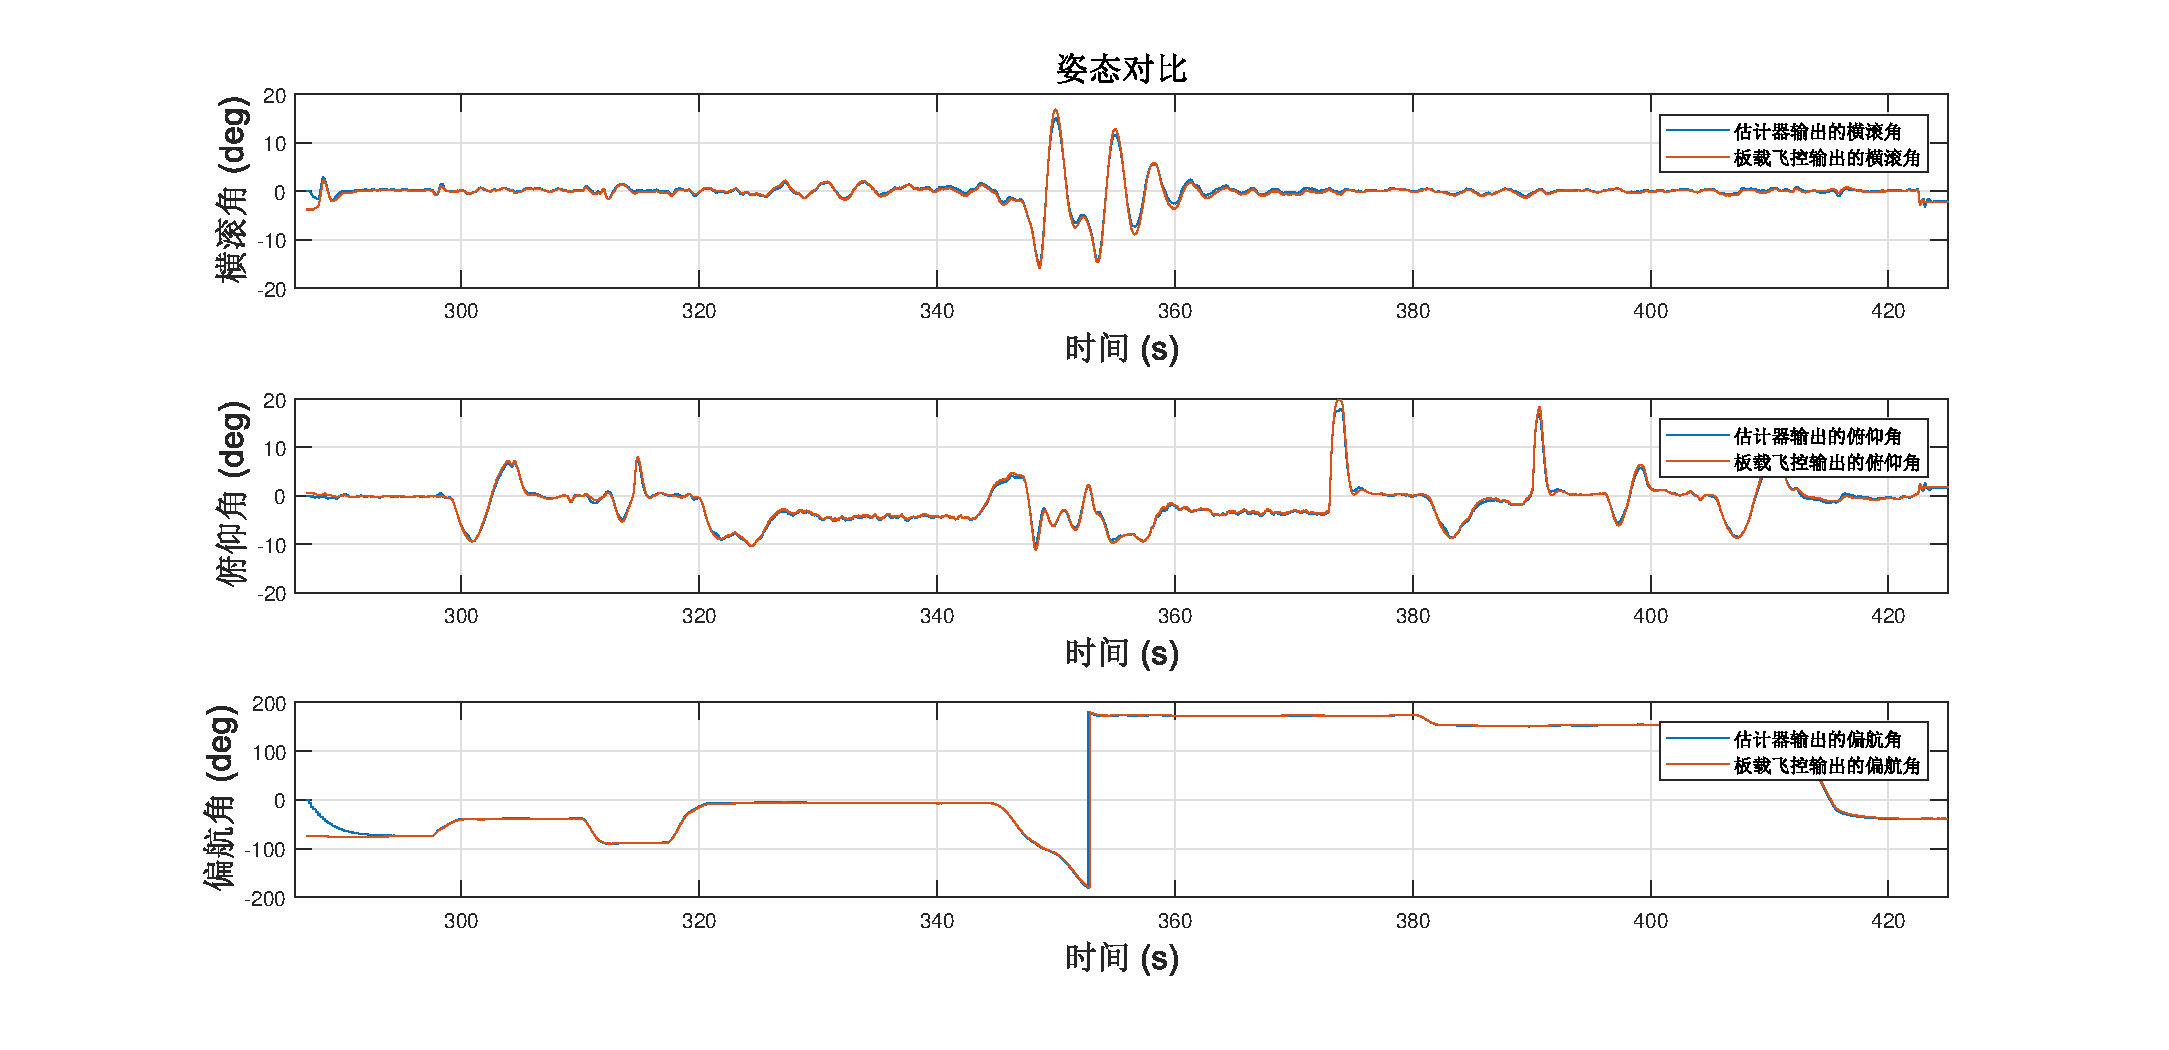
\includegraphics[width=1.0\textwidth]{attitude4.eps}
	\bicaption{姿态对比}{Attitude comparison}
	\label{fig:attitude}
\end{figure} 
%\autoref{fig:attitude}给出了飞行过程中本文算法以及板载飞控输出的欧拉角曲线。
从\autoref{fig:attitude}可以看出,本算法估计的姿态和板载飞控板给出的姿态基本一致,表明估计姿态能收敛到真实姿态。

%RTK能输出世界坐标系下的位置和速度。
本文的估计器以及RTK输出的三维位置、速度对比曲线如\autoref{fig:velocity}和\autoref{fig:position}所示。
\begin{figure}[H]
	\centering
	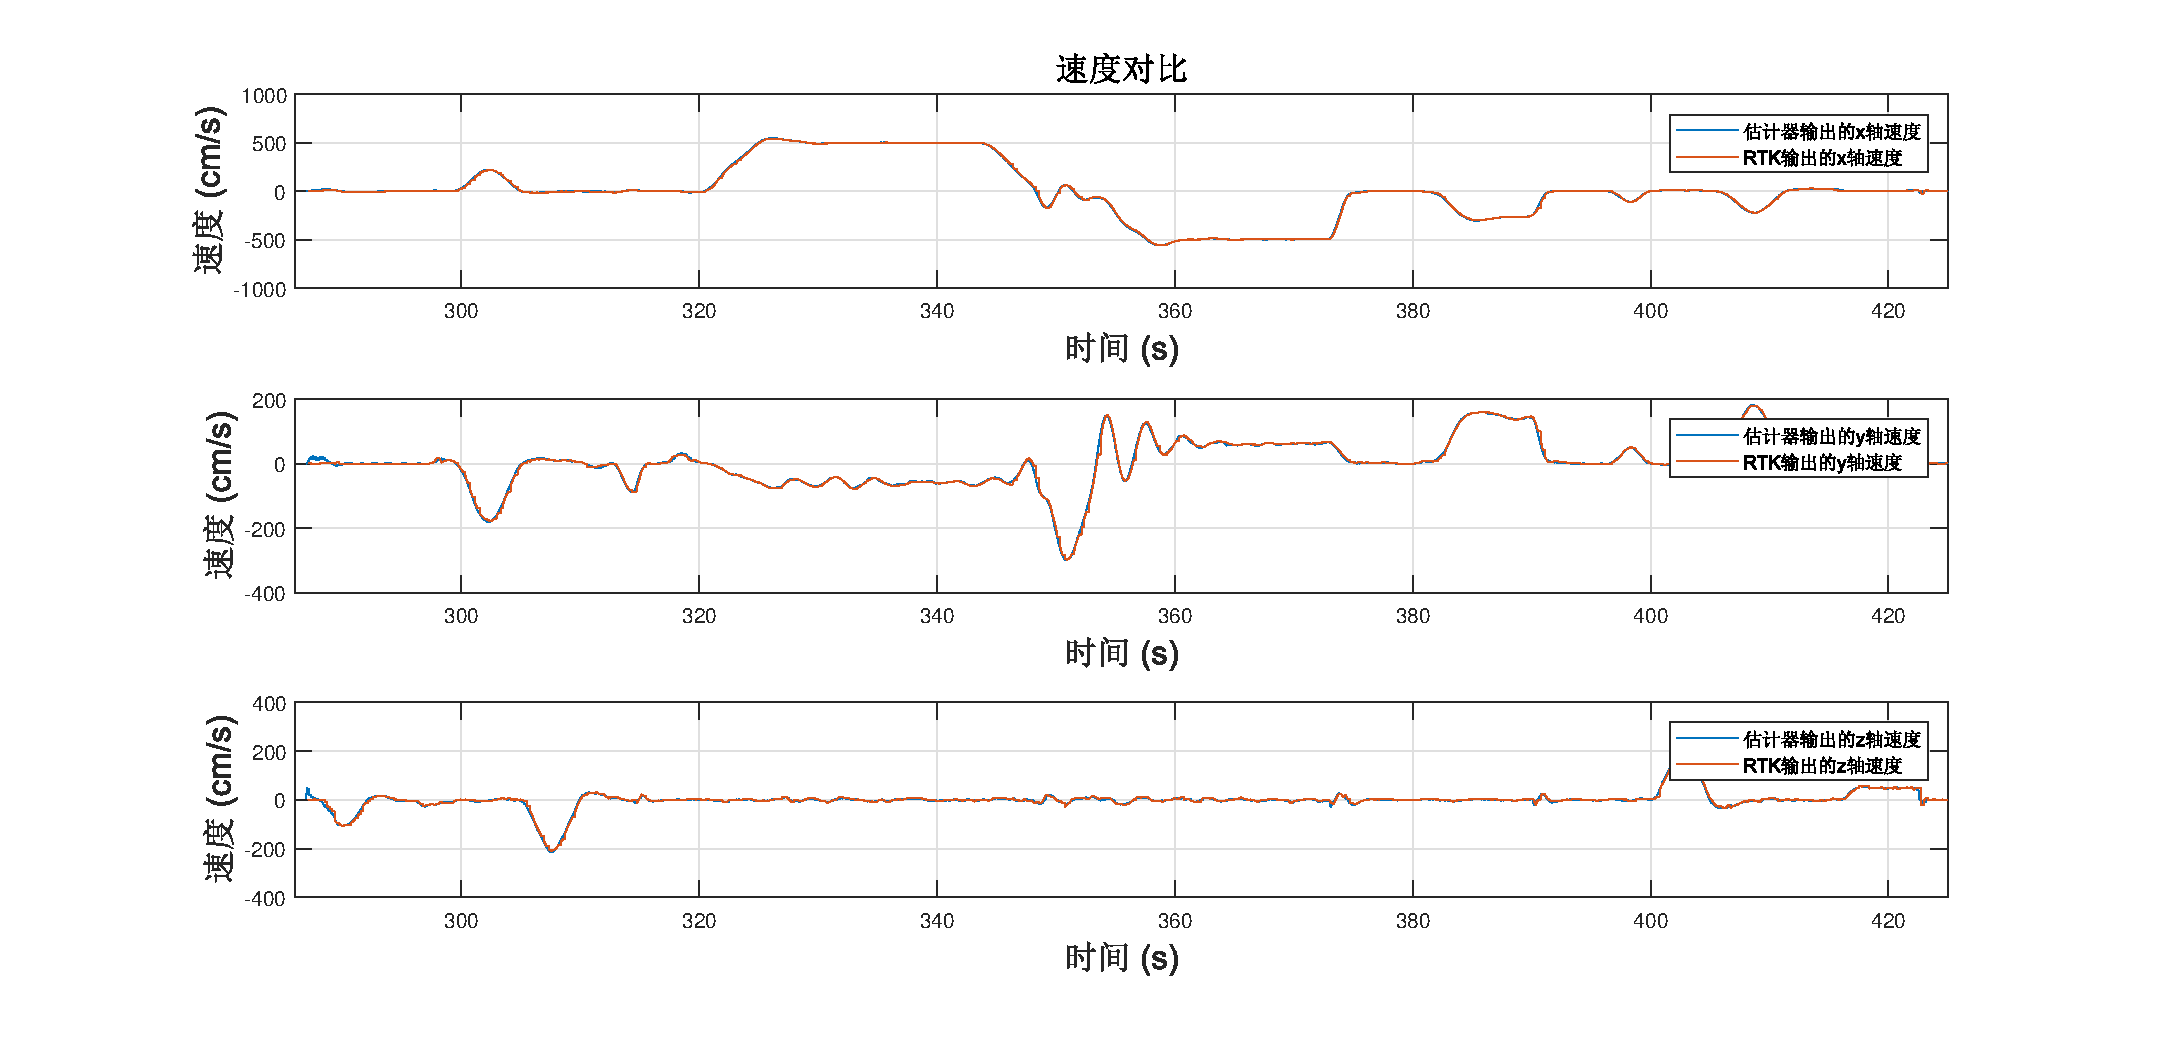
\includegraphics[width=1.0\textwidth]{velocity3.eps}
	\bicaption{速度对比}{Velocity comparison}
	\label{fig:velocity}
\end{figure}

\begin{figure}[H]
	\centering
	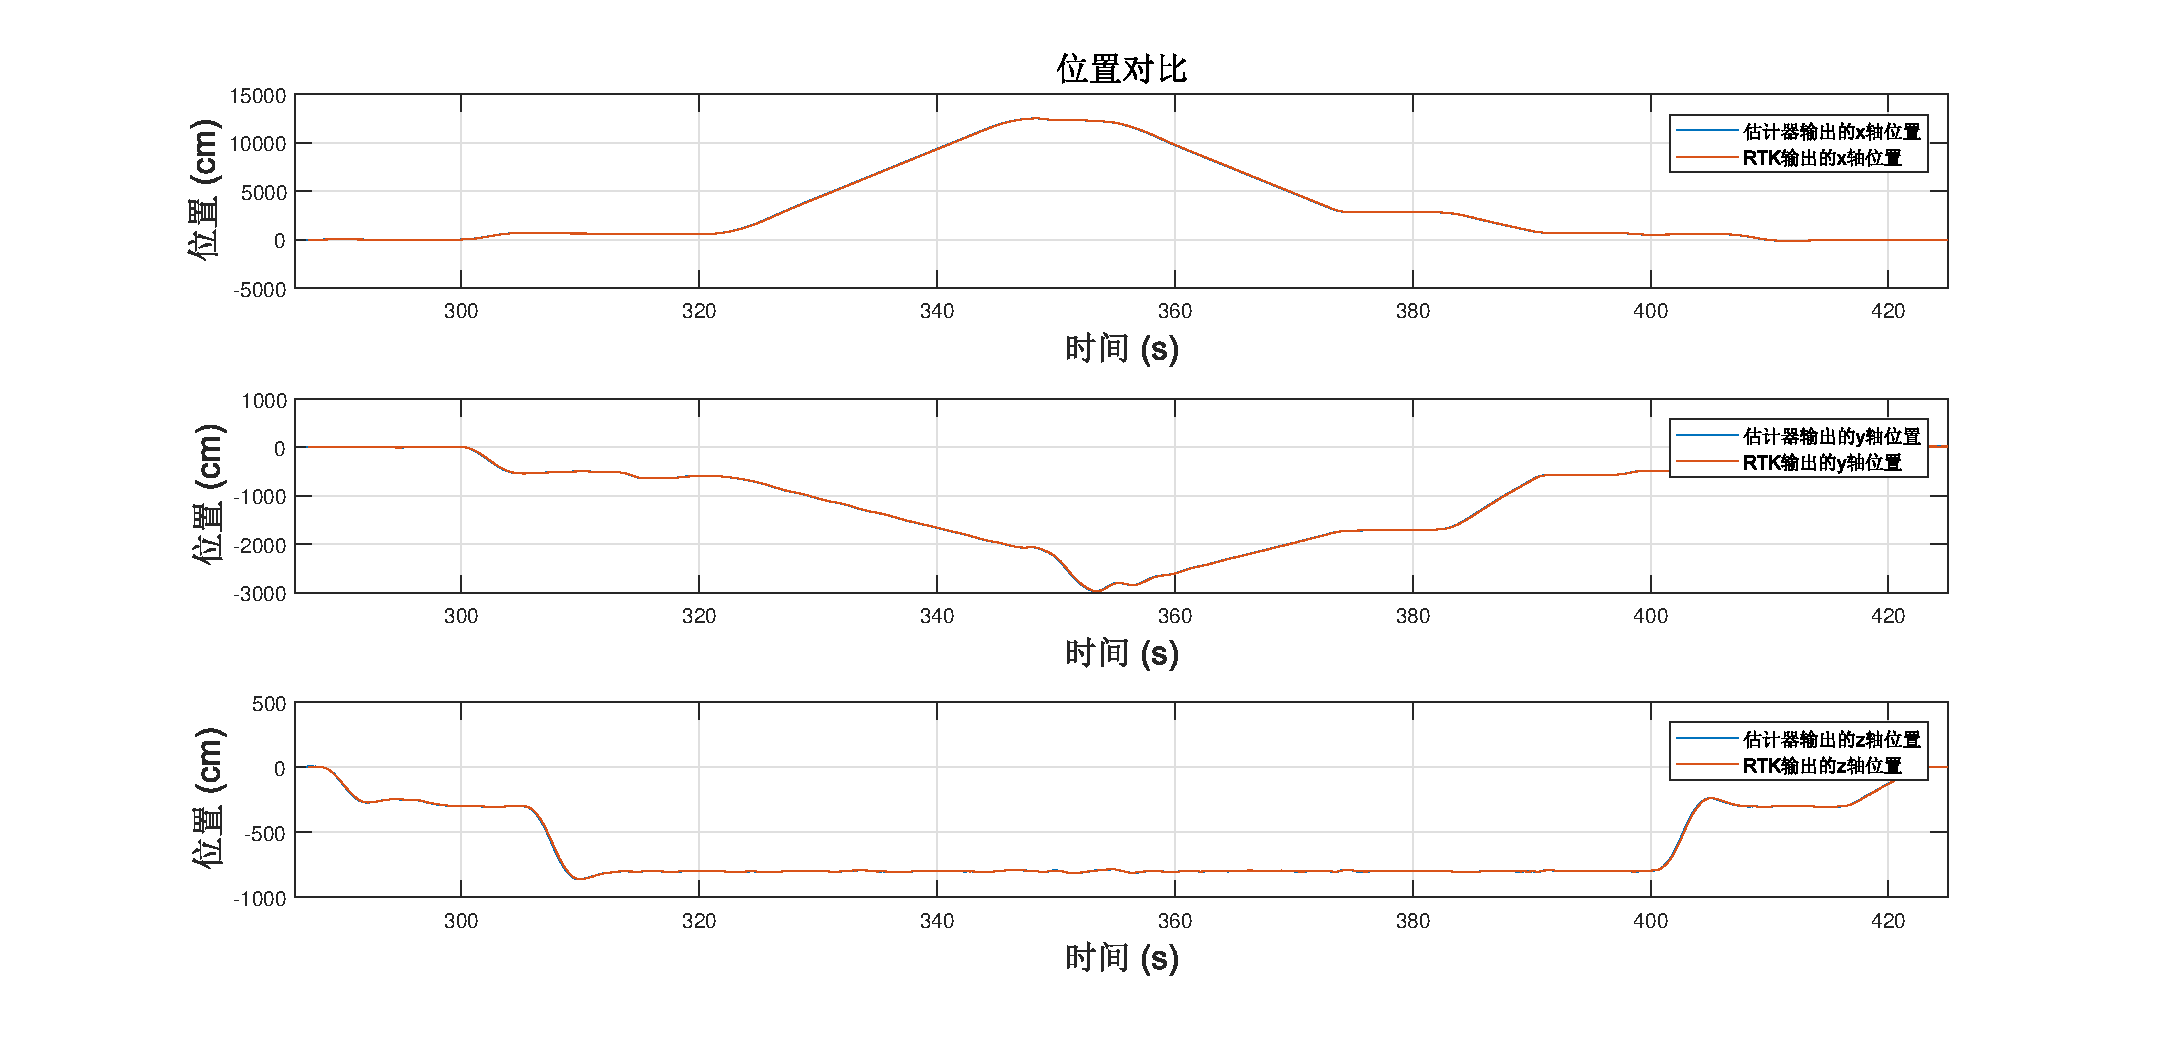
\includegraphics[width=1.0\textwidth]{position3.eps}
	\bicaption{位置对比}{Position comparison}
	\label{fig:position}
\end{figure}
%此外,可以通过对比估计器输出的位置、速度和RTK输出的位置、速度的一致性进而评估位置融合的效果。
从\autoref{fig:velocity}、\autoref{fig:position}可以看出,本算法估计的位置和速度和RTK给出的位置和速度基本一致,表明估计位置和速度能收敛到真实位置和速度。
\begin{figure}[H]
	\centering
	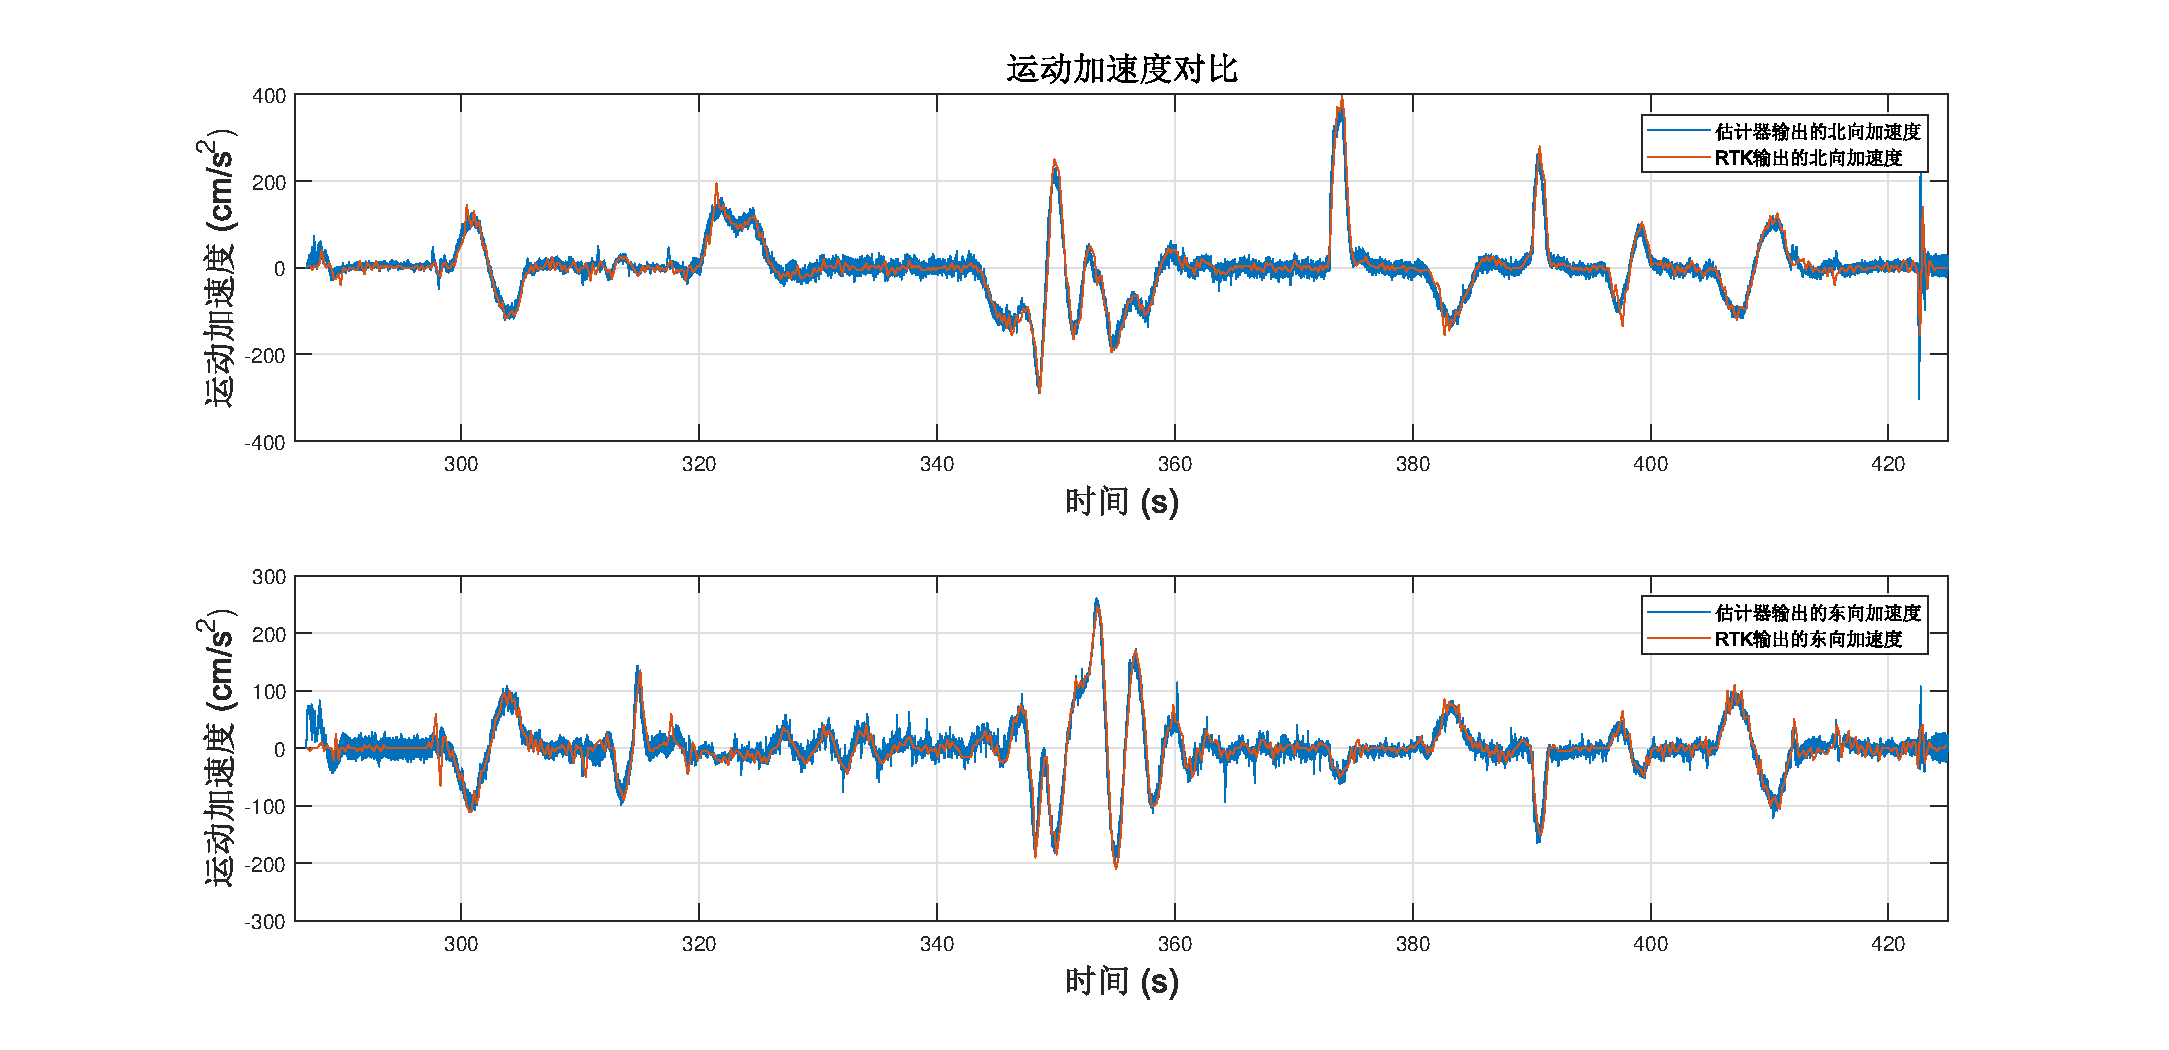
\includegraphics[width=1.0\textwidth]{motionacc3.eps}
	\bicaption{运动加速度对比}{Motion acceleration comparison}
	\label{fig:motionacc}
\end{figure}

此外,对于姿态,可以使用运动加速度间接计算估计器的精确度,通过分析二者的误差进而评估估计器的性能指标。
本实验首先通过估计器输出的姿态求出估计器输出的运动加速度,然后通过RTK输出的速度差分求出RTK输出的运动加速度。
本文估计器计算的运动加速度以及通过差分RTK计算的运动加速度对比曲线如\autoref{fig:motionacc}所示。
从\autoref{fig:motionacc}可以看出,本算法估计的运动加速度和RTK给出的运动加速度基本一致,进一步表明姿态估计是收敛的。

飞行过程中本文算法计算的三维飞行轨迹以及RTK输出的飞行轨迹对比曲线如\autoref{fig:trajectory}所示。
三维轨迹对比表明系统在快速机动一段较长的时间内能无故障稳定运行。
\begin{figure}[H]
	\centering
	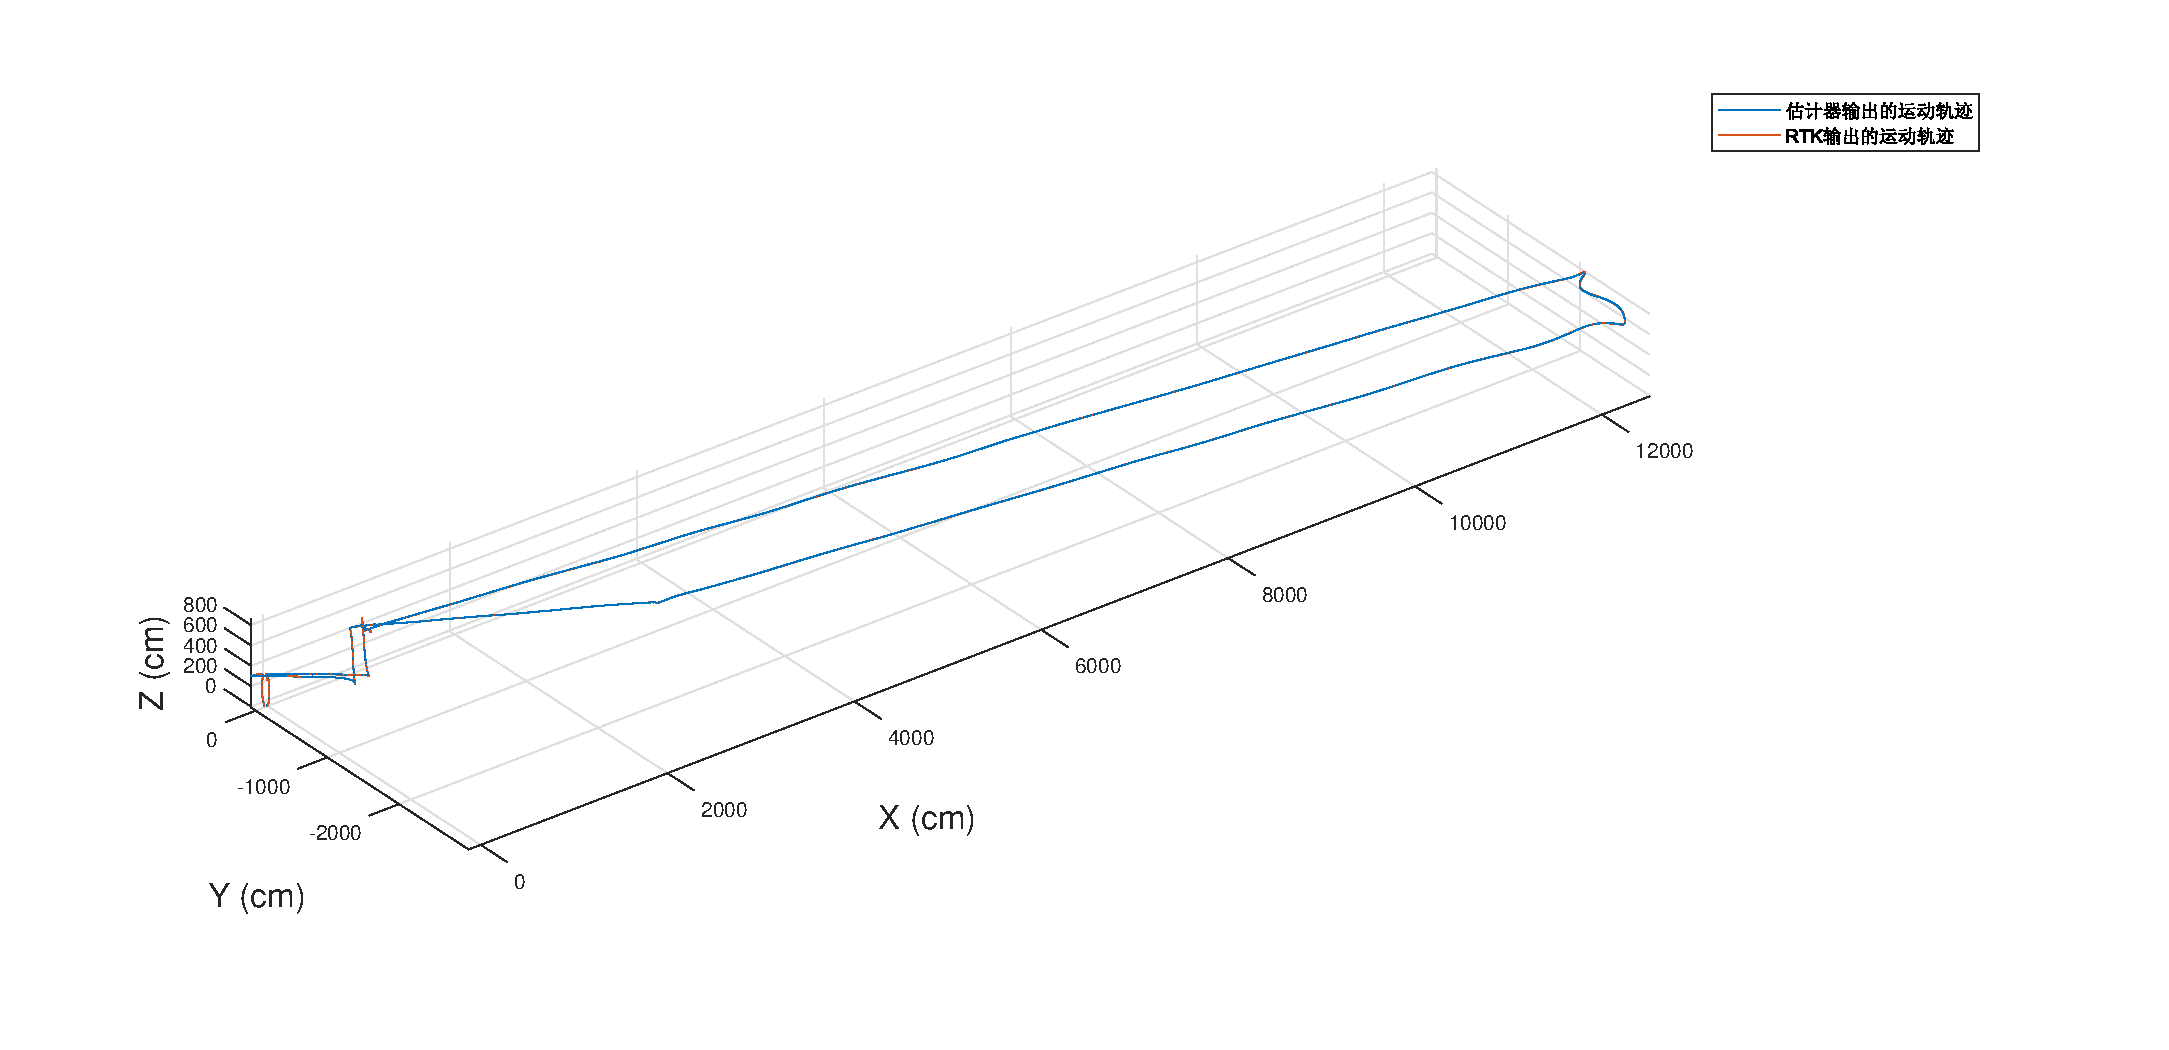
\includegraphics[width=1.0\textwidth]{trajectory2.eps}
	\bicaption{飞行轨迹}{Flight trajectory}
	\label{fig:trajectory}
\end{figure}
%\autoref{fig:trajectory}给出了飞行过程中本文算法计算的三维飞行估计以及RTK输出的位置轨迹,表面系统在快速机动一段较长的时间内能无故障稳定运行。

最后,本实验通过采用标准差来评估估计器的性能。
其中,运动加速度的标准差记为$\big\{ \sigma_{a_x},\sigma_{a_y} \big\}$,
偏航角$\psi$的标准差记为$\sigma_{\psi}$,
位置的标准差记为$\big\{ \sigma_{p_x},\sigma_{p_y},\sigma_{p_z} \big\}$,
速度的标准差记为$\big\{ \sigma_{v_x},\sigma_{v_y},\sigma_{v_z} \big\}$。
相关状态量标准差计算结果如\autoref{stdestimate}所示。
\begin{table}[H]
	\bicaption{估计值标准差}{Standard error of estimation}
	\label{stdestimate}
	\begin{tabular}{cc}
		\toprule
		状态量 & 标准差 \\
		\midrule
		$\big\{ \sigma_{a_x},\sigma_{a_y} \big\}$ & $\big\{ 14.61, 15.28 \big\}$(cm/s) \\
		$\sigma_{\psi}$ & $0.23$($^{\circ}$)   \\
		$\big\{ \sigma_{p_x},\sigma_{p_y},\sigma_{p_z} \big\}$ & $\big\{ 3.21, 1.37, 1.44 \big\}$(cm)   \\
		$\big\{ \sigma_{v_x},\sigma_{v_y},\sigma_{v_z} \big\}$ & $\big\{ 3.37, 3.31, 4.26 \big\}$(cm/s)   \\
		\bottomrule
	\end{tabular}
\end{table}

结合上述评价指标分析可得出以下结论:

(1)本算法估计的位置、速度以及运动加速度和RTK输出的位置、速度以及运动加速度基本一致,表明算法整体是收敛的。

(2)飞行轨迹涉及到大机动刹车和姿态变化,这时姿态和速度依然能够跟踪上真值,表明算法的运动加速度延时补偿是有效的。

(3)可见运动加速度的标准差最大为$15.28cm/s^2$,说明姿态误差不超过$1^{\circ}$,位置和速度的标准差均能达到飞行精度的要求。

\gdutsubsection{传感器干扰下估计器的性能评估}{Performance evaluation of estimators under sensor interference}
通过第一个实验可以证明本文的融合算法是可以达到要求的。
接下来通过实验验证系统的鲁棒性。
第二个实验则在不同环境下测试了系统的鲁棒性和安全性。

为了验证算法能否有效地抑制运动加速度,本实验让飞行器进行大幅度的姿态变化运动。
如\autoref{fig:motionaccdelay}所示,本实验比对了本文估计器、板载飞控、标准ECF算法以及加速度计输出的姿态来评估估计器的鲁棒性。
%如\autoref{fig:motionaccdelay}所示
\begin{figure}[H]
	\centering
	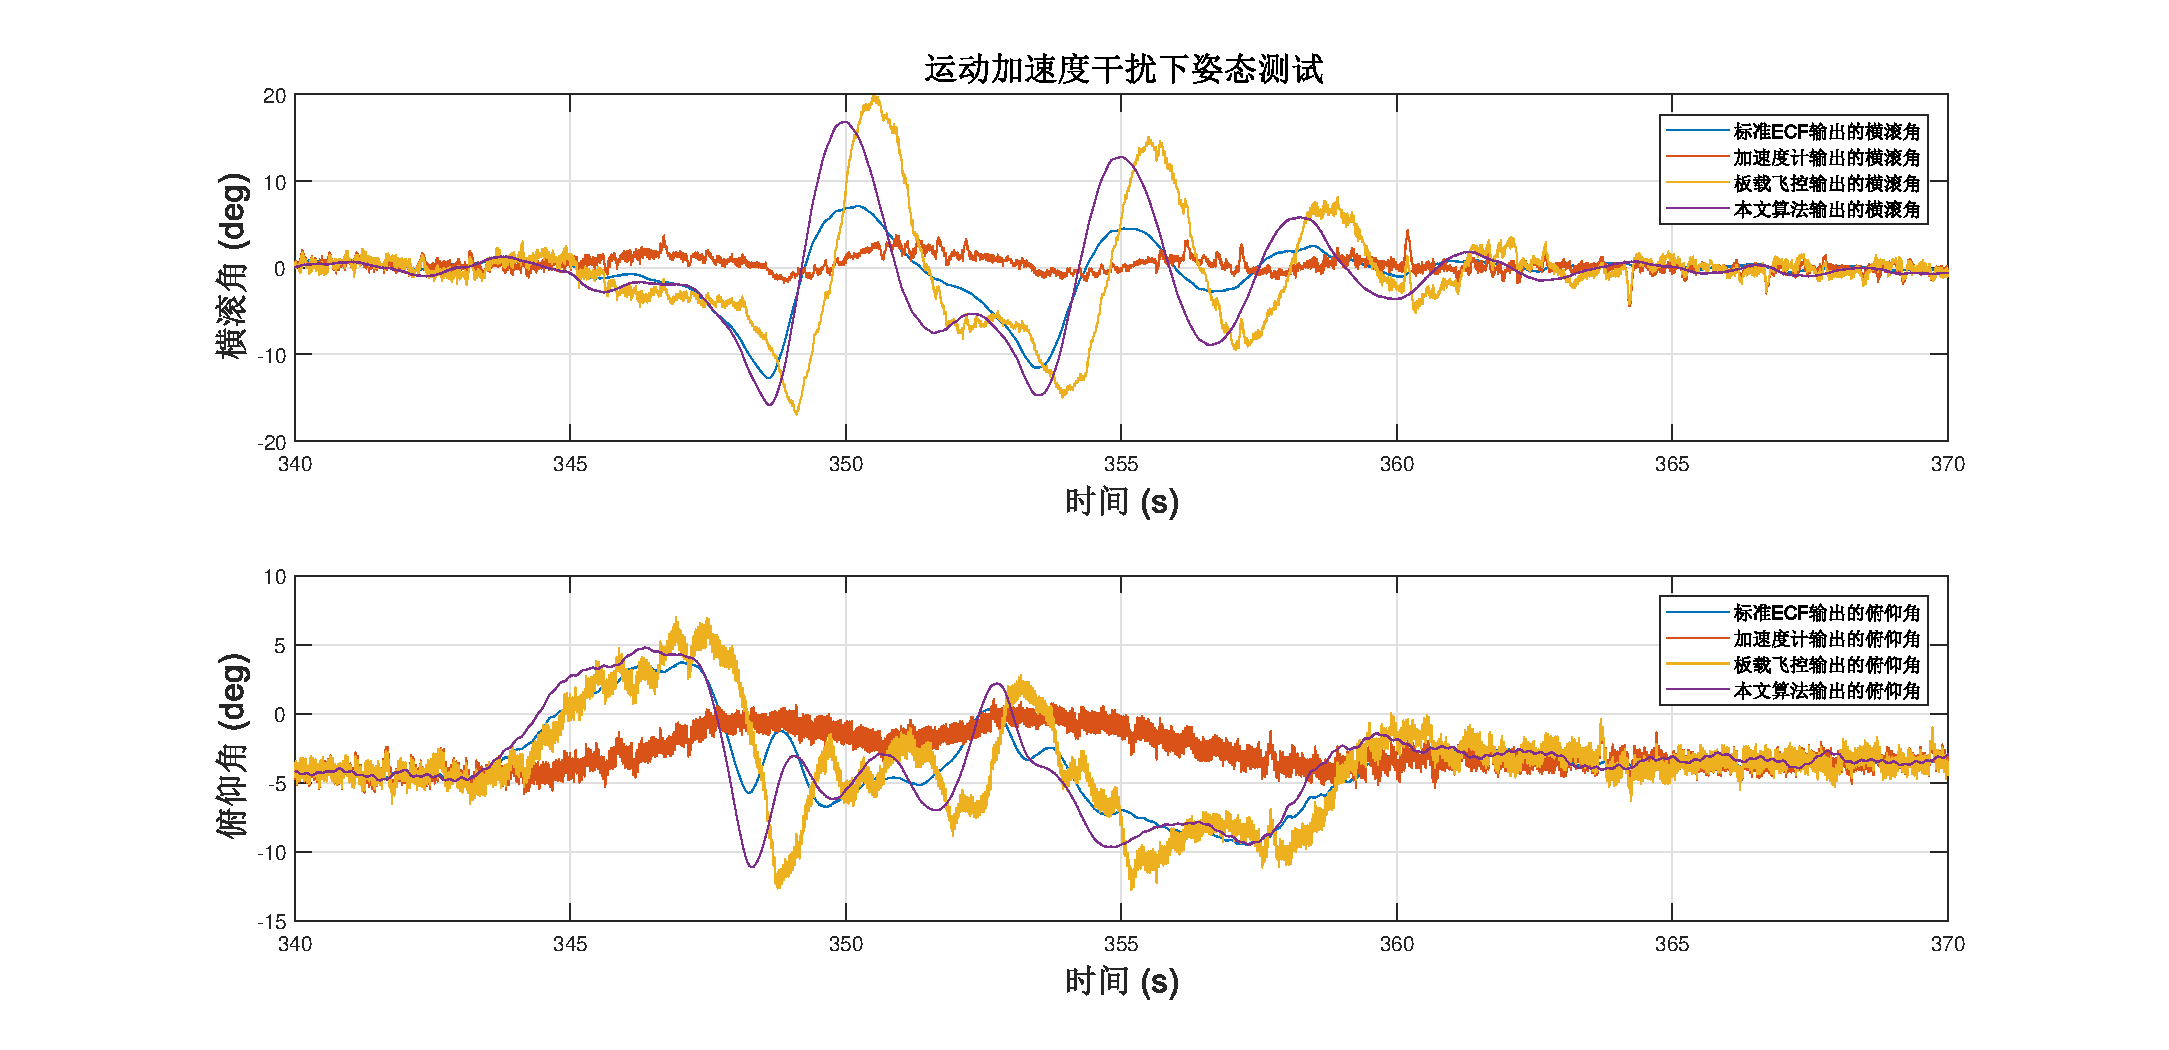
\includegraphics[width=1.0\textwidth]{motionaccdelay2.eps}
	\bicaption{高机动环境下的姿态对比}{Attitude comparison in high maneuvering environment}
	\label{fig:motionaccdelay}
\end{figure}

从\autoref{fig:motionaccdelay}可得出以下结论:

(1)在高机动环境下标准显式互补滤波器的输出性能较差,在某些时刻姿态角偏离真实角度约有10度。

(2)在高机动环境下加速度计的输出基本无法作为参考值。

(3)本文的估计器输出与板载飞控输出基本一致,并且能做到相位超前。

%这里需要说明的是,为了做到能处理扰动,需要要求每个传感器需要有对应的故障诊断机制。
%本文工作的一个目标让开发人员能方面的针对传感器扰动加入对应的异常处理算法。
%传感器干扰包括但不限于气压计干扰、磁场干扰、GPS信号异常等。
为了验证算法能否有效地抑制磁场干扰,本实验在飞控旁边放置一块磁铁作为干扰源。
%磁力计在受到外部磁场干扰时会严重影响到偏航角$\psi$的估计。
%在本实验中,我们模拟这种干扰的出现。
在偏航角受干扰情况下,依靠本文提出的融合框架,可以对磁场异常做出判断,将修正部分隔离,能保证总体融合结果的平滑准确。
如\autoref{fig:yaw}所示,本实验比对了本文估计器融合后的偏航角、预测偏航角以及磁力计计算的偏航角。
%实验结果如\autoref{fig:yaw}所示。
\begin{figure}[H]
	\centering
	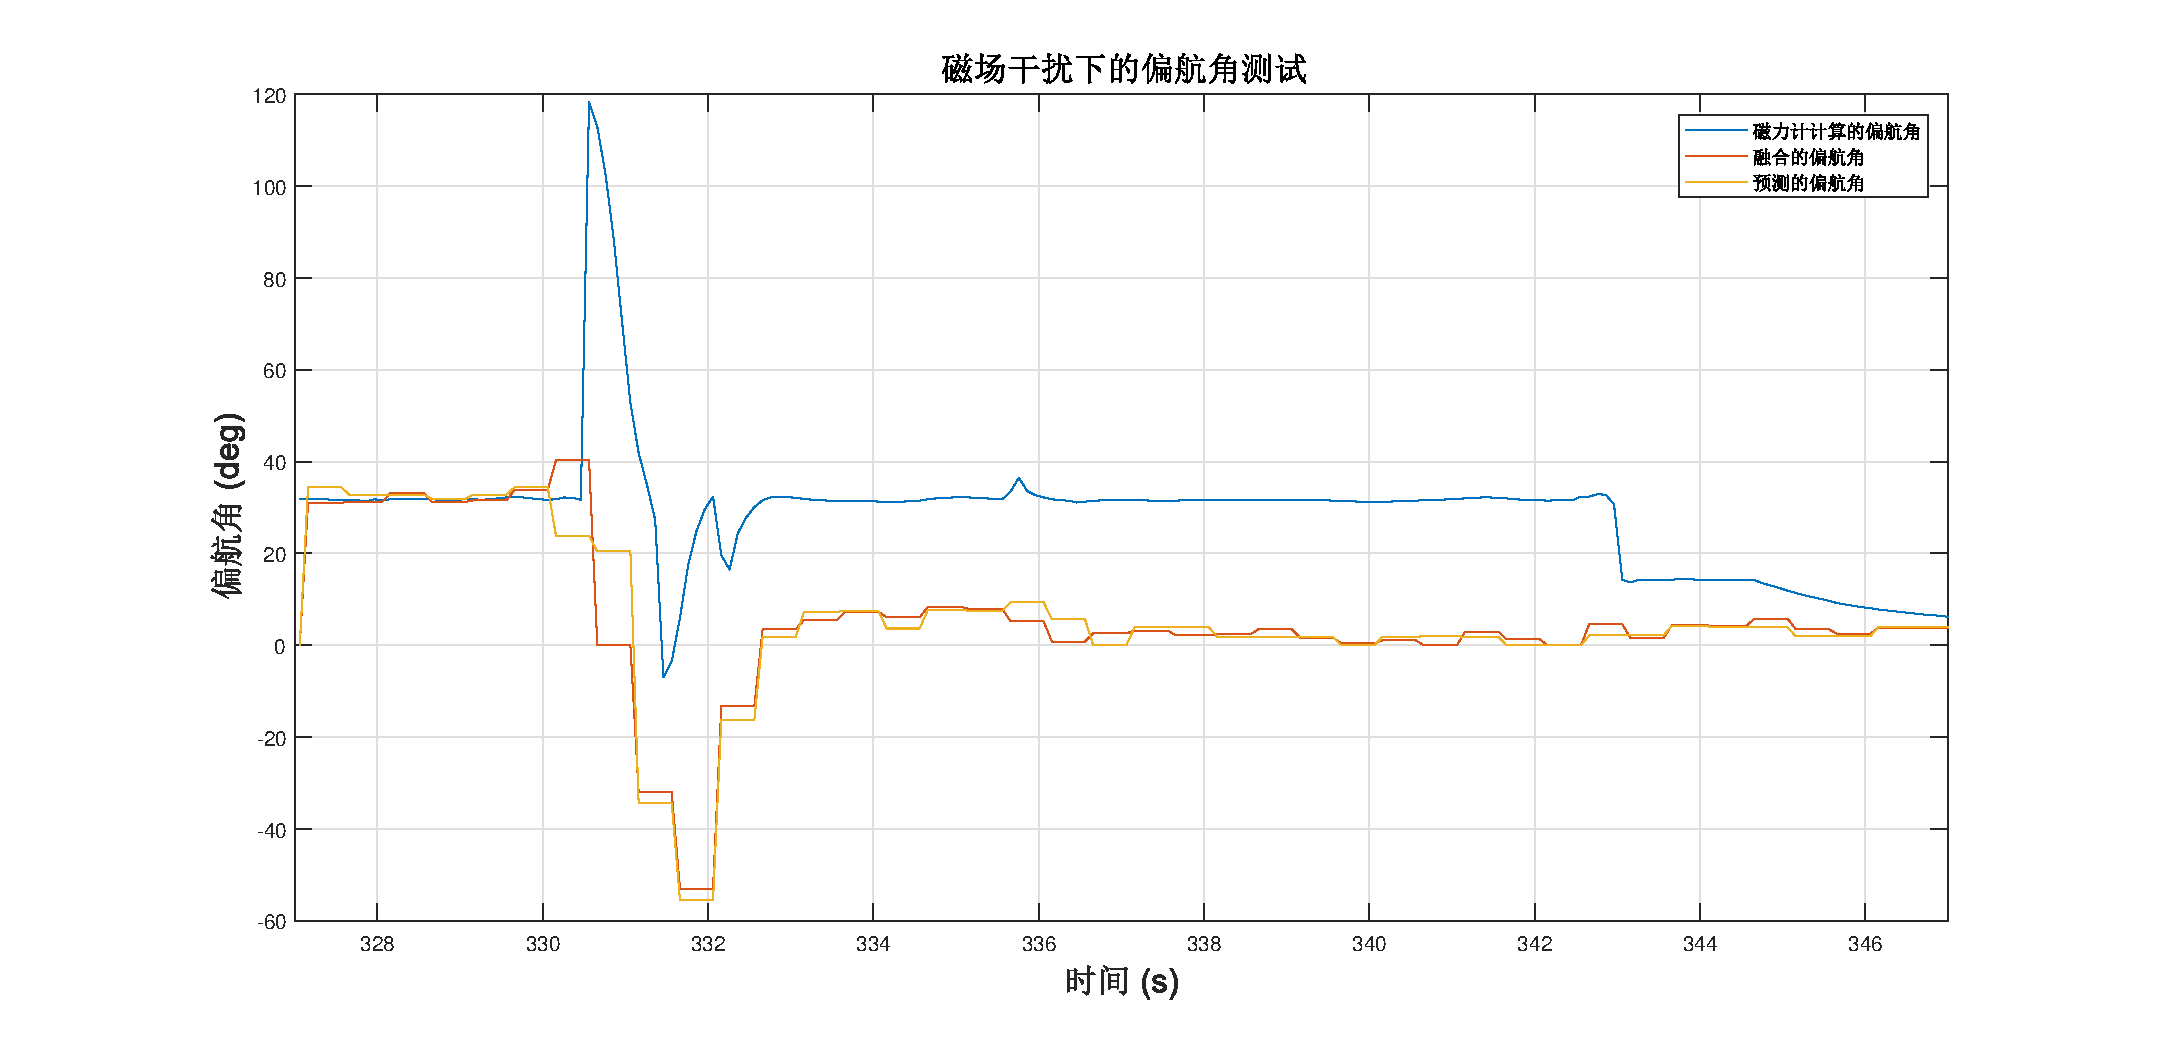
\includegraphics[width=1.0\textwidth]{yaw2.eps}
	\bicaption{磁场干扰下的偏航角估计}{Estimation of yaw Angle under magnetic field disturbance}
	\label{fig:yaw}
\end{figure}

从\autoref{fig:yaw}可得出以下结论:

(1)给系统施加持续15s的扰动,可以观察到由磁力计解算的偏航角是完全错误的。

(2)使用阈值判断出异常后可以将修正项隔离,避免磁场干扰的影响。

(3)对比融合偏航角和预测偏航角可以发现二者是存在一定误差的,在没有修正项存在的情况下不可避免,但是整体误差不会很大。

\gdutsection{总结与讨论}{Summary and discussion}
本章使用IMU作为主要传感器,融合其他传感器进行状态估计以实现飞行器的稳定飞行。
针对传感器具有多频率多延时的特性,难以处理多源信息融合的问题,提出了预测-修正-延时融合框架,能随意添加或减少传感器,解决了多源信息融合困难的问题。
针对运动加速度延时不准确以及磁场干扰影响横滚角、俯仰角的问题,提出了解耦策略以及运动加速度插值延时补偿算法,解决了来自加速度计和磁力计的传感器干扰的问题。
本文提出的算法作为状态估计模块满足飞行器稳定飞行的需求。

本文注意到,滤波器框架并不是融合多传感器的唯一方法。
在基于图的框架中对多传感器融合也是很简单的,因为每个测量结果只是向图中添加另一个边缘或因子节点\cite{schleicher2009real}。
然而,由于传感器融合的结果直接用于飞行器的反馈控制,基于图的方法存在较大的延迟和计算复杂度,不适合本课题的应用。

另一方面,本文提出的预测-修正-延时融合框架是一个松耦合的融合方法。
由于本方法的解耦的特点,它使不同传感器的组合变得容易。
这种松耦合的方法也使得传感器融合框架具有计算轻量化的特点。
因此,本方法非常适合于对实时性要求高的系统。

然而,为了做到能处理扰动,需要要求每个传感器需要有对应的故障诊断机制。
这些处理机制的合理性对整体融合性能至关重要。
本文的传感器融合框架忽略了测量值之间的耦合,与紧耦合方法相比,算法的融合结果可能会在精度上有所损失\cite{indelman2013incremental}。
但需要强调的是,对于飞行器的反馈控制,安全性比精度更重要。
对于这些应用场景,本文的方法仍然为复杂的传感器融合问题提供了一个可行的和易于使用的解决方案。

\gdutchapter{多旋翼飞行器控制方法}{Control method for multi-rotor aircraft}
基于第三章描述的状态估计方法,本章将讨论如何设计控制算法,以验证本文提出的状态估计方法的有效性。
本章首先展示多旋翼飞行器的动力学模型,然后重点介绍了控制框架以及控制律的设计,最后给出飞行测试结果。

\gdutsection{多旋翼飞行器动力学模型}{Dynamics model of multi-rotor aircraft}
首先进行符号约定以便进行公式推导。
将目标状态量和误差状态量分别定义为$(\cdot)_d$和$(\cdot)_e$。
记$k_{(\cdot)}$为控制律中的增益参数。

考虑\autoref{fig:modelaerialrobot}中所示的多旋翼飞行器模型。
这是一个由四个相同的电机和螺旋桨组成的系统。
通过螺旋桨产生的推力和扭矩垂直于飞行器所在平面。
%机体坐标系的原点位于飞行器的质心。

基于这个模型,定义如下物理量

$m \in \mathbb{R}$,表示飞行器总质量;

$J \in \mathbb{R}^{3 \times 3}$,表示在机体坐标系下的转动惯量矩阵;

$R \in SO(3)$,表示从机体坐标系到世界坐标系的旋转矩阵;

$\omega^b \in \mathbb{R}^3$,表示在机体坐标系下的角速度;

$x \in \mathbb{R}^3$,表示在世界坐标系下的飞行器质心的位置;

$v \in \mathbb{R}^3$,表示在世界坐标系下的飞行器质心的速度;

$f \in \mathbb{R}$,表示螺旋桨沿电机轴产生的总推力;

$\tau \in \mathbb{R}^3$,表示在机体坐标系下的螺旋桨产生的总力矩;

基于以上定义,多旋翼飞行器的运动方程可以写成\vspace{1ex}
\begin{gather}\label{eq:dynamics}
	\dot{x} = v\\
	m\dot{v} = mge_3 - fRe_3\\
	\dot{R} = R\hat{\omega}^b\\
	J\dot{\omega}^b + \omega^b \times J \omega^b = \tau
\end{gather}

\gdutsection{控制算法分析}{Control algorithm analysis}
在获得了飞行器的状态后,可以使用各种现有的控制策略使飞行器稳定飞行。
线性控制器,如PID控制器或LQR控制器,被广泛应用于多旋翼飞行器中\cite{mechali2022fixed,elkhatem2022robust}。。
在飞行器工作接近悬停状态的假设下,对于低速运行、加速度变化小的飞行器,可以使用线性控制器。
针对多旋翼飞行器在执行器饱和情况下的线性化动力学问题,Guenard等人设计了一种非线性控制器\cite{guenard2005dynamic}。
%针对四旋翼无人机在饱和位置下的线性化动力学问题,Guenard等人设计了一种非线性控制器\cite{guenard2005dynamic}。
文献\parencite{bouabdallah2005backstepping}中应用了反步和滑模技术。
以上所提到的控制器是基于欧拉角设计的,它们在表示多旋翼飞行器复杂的旋转运动时表现出奇点,从而从根本上限制了它们跟踪轨迹的能力。
基于李群上的刚体动力学描述,Lee等人设计了一种应用在四旋翼飞行器的几何控制器,并证明了几乎全局稳定性\cite{lee2010geometric}。
对于包含大姿态变化的运动,几何控制器是更合适的选择。
本文基于文献\parencite{lee2010geometric}的控制方法进行设计,完成了飞行控制系统的闭环。

\gdutsection{控制算法设计}{Control algorithm design}
%针对多旋翼飞行器的非线性耦合系统,本文设计了一个控制器跟踪目标轨迹。

\gdutsubsection{控制框架}{Control scheme}
多旋翼飞行器是一个欠驱动系统。
由多旋翼飞行器的动力学模型可知,飞行器是通过总拉力$f$和三轴力矩$\tau$控制位置$x$和姿态$R$。
%具体通过总拉力$f$和三轴力矩$\tau$控制位置$x$和姿态$R$。
本文采用串级控制策略设计多旋翼飞行器,将控制器分为位置控制器和姿态控制器。
通过串级控制实现多旋翼飞行器的升降、悬停、侧飞等飞行模态。
控制器可以分层的原因是多旋翼飞行器的结构特点:姿态是使用力矩作为控制输入调节。
因此姿态可以单独作为内环处理。
运动方程(\autoref{eq:dynamics})具有级联结构。
姿态的转动运动与平动运动解耦。
平动只依赖于公式(5.3)中的$fRe_3$项。
总推力$f$的大小是直接控制的,而总推力$Re_3$的方向是由机体轴$\vec{b}_3$决定的。
因此,为了改变总推力的方向,应相应地改变姿态。
因此选择所需的总推力$f$以及目标姿态$R_d e_3$作为输入跟踪位置$x_d$。
控制力矩$\tau$作为输入跟踪目标姿态$R_d$。
控制器总体框架如\autoref{fig:controllerstructure}所示。
\begin{figure}[H]
	\centering
	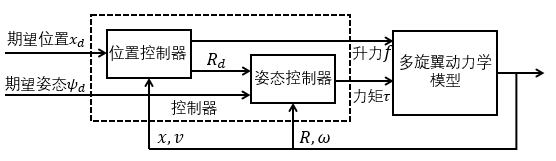
\includegraphics[width=0.9\textwidth]{屏幕截图 2022-06-08 121234.png}
	\bicaption{控制框架图}{Controller structure}
	\label{fig:controllerstructure}
\end{figure}

%\gdutsubsection{位置控制}{Position controln}
%根据输出目标状态的不同,位置控制分为两种方法。
%一种方法是产生期望欧拉角的位置控制。
%针对线性系统设计控制器。
%这种类型的位置控制器最终产生的期望值为欧拉角和拉力$\phi_d,\theta_d,f_d$。
%另一种方法是产生期望旋转矩阵的位置控制。
%直接针对非线性耦合系统设计控制器。这种类型的位置控制器最终产生的期望值为旋转矩阵和拉力$R_d,f_d$。
%本文采用产生期望旋转矩阵的位置控制方法进行设计,最后使用四元数作为期望姿态的表示。
%可进一步将位置控制器解耦成水平控制器和高度控制器。
%水平控制器输出目标姿态$q_d$(四元数表示),高度控制器输出推力$f$。
%记需要跟踪给定位置为$x_d$。
%求目标加速度
%\begin{gather}
%	v_d = k_x (x_d - x)\\
%	a_d = k_v (v_d - v)
%\end{gather}
%将目标加速度要从世界坐标系转换到$bodyheading$坐标系:\vspace{1ex}
%\begin{gather}
%a_d^{bodyheading} = q_{\psi} \otimes a_d \otimes (q_{\psi})^{*}
%\end{gather}
%由目标加速度计算目标角度
%\begin{gather}
%	\phi_d = atan(\frac{a_{dy}^{bodyheading}}{a_z})\\
%	\theta_d = atan(\frac{a_{dx}^{bodyheading}}{a_z})
%\end{gather}
%构造目标四元数
%\begin{gather}
%	q_d = q_{\psi_d} \otimes q_{\theta_d} \otimes q_{\phi_d}
%\end{gather}
%
%下面进一步考虑期望拉力$f_d$的计算。
%对于拉力的生成,由目标的z轴运动加速度到目标拉力之间的关系可由下式确定:\vspace{1ex}
%\begin{gather}\label{eq:AltitudeControl}
%	f = \frac{ma_{dz} + f_0 cos\theta_0 cos\phi_0}{cos\theta cos\phi}
%\end{gather}
%其中,$f_0 cos\theta_0 cos\phi_0$表示了悬停油门。
%\autoref{eq:AltitudeControl}的$1/cos\theta cos\phi$这一项为油门倾角补偿,因为高度控制计算出的$f$为竖直方向上的期望升力,需要投影到机体坐标系得到旋翼产生的总升力。
%以上是位置控制器的控制律设计。
%
%\gdutsubsection{姿态控制}{Attitude control}
%多旋翼采用内外层控制,外层控制器为内层控制器提供指令,即把位置通道控制器的输出($R_d$)作为姿态控制系统的参考值。
%后续的姿态控制的目标是实现姿态误差收敛到0。
%因此,剩余的控制目标就传给了姿态控制。
%只要姿态控制被很好地实现,水平位置跟踪的问题就可以被解决。
%
%求误差四元数\vspace{1ex}
%\begin{gather}\label{eq:errquat}
%	q_e = q_d \otimes q^{*} = q_0 + v_e
%\end{gather}
%\autoref{eq:errquat}中$v_e = q_1 i + q_2 j + q_3 k$。
%由四元数定义,姿态误差为$\sigma_e = 2acos(q_0)$,世界坐标系下的姿态误差表示为
%\begin{gather}
%	e^w = \frac{\left| v_e \right|}{sin\frac{\sigma_e}{2}} v_e
%\end{gather}
%机体坐标系下的目标角速度表示为
%\begin{gather}
%	\omega^b_d = k_q q \otimes e^w \otimes q^{*}
%\end{gather}
%角速度控制
%\begin{gather}\label{eq:angularacontrol}
%	\omega^b_e = \omega^b_d - \omega^b\\
%	\dot{\omega}^b_d = k_{p \omega} \omega^b_e + k_{d \omega} \frac{d}{dt}\omega^b_e
%\end{gather}
%角加速度控制
%\begin{gather}\label{eq:angularaccelerationcontrol}
%		\dot{\omega}^b_e = \dot{\omega}^b_d - \dot{\omega}^b\\
%		\tau = k_{p \tau} \dot{\omega}^b_e + k_{i \tau} \int_{0}^{t}\dot{\omega}^b_e + \omega^b \times J \omega^b
%\end{gather}

\gdutsubsection{控制律设计}{Control law design}
控制器的目标是实现轨迹跟踪,使飞行器的轨迹贴合给定的轨迹。
根据\autoref{fig:controllerstructure}展示的控制框架,控制器可以分为位置控制器和姿态控制器两部分。
对于位置控制器,本文应用文献\parencite{lee2010geometric}提出的几何方法进行设计。
基于几何方法设计的位置控制器最终产生的目标值为旋转矩阵$R_d$和拉力$f$。
可进一步将位置控制器解耦成水平控制器和高度控制器。
水平控制器输出目标姿态$q_d$(四元数表示),高度控制器输出推力$f$。
记需要跟踪给定位置为$x_d$。
求目标加速度
\begin{gather}
	v_d = k_x (x_d - x)\\
	a_d = k_v (v_d - v)
\end{gather}
将目标加速度要从世界坐标系转换到$bodyheading$坐标系:\vspace{1ex}
\begin{gather}
a_d^{bodyheading} = q_{\psi} \otimes a_d \otimes (q_{\psi})^{*}
\end{gather}
由目标加速度计算目标角度
\begin{gather}
	\phi_d = atan(\frac{a_{dy}^{bodyheading}}{a_z})\\
	\theta_d = atan(\frac{a_{dx}^{bodyheading}}{a_z})
\end{gather}
构造目标四元数
\begin{gather}
	q_d = q_{\psi_d} \otimes q_{\theta_d} \otimes q_{\phi_d}
\end{gather}
对于拉力的生成,由目标的z轴运动加速度到目标拉力之间的关系可由下式确定:\vspace{1ex}
\begin{gather}\label{eq:AltitudeControl}
	f = \frac{ma_{dz} + f_0 cos\theta_0 cos\phi_0}{cos\theta cos\phi}
\end{gather}
其中,$f_0 cos\theta_0 cos\phi_0$表示了悬停油门。
\autoref{eq:AltitudeControl}的$1/cos\theta cos\phi$这一项为油门倾角补偿,因为高度控制计算出的$f$为竖直方向上的期望升力,需要投影到机体坐标系得到旋翼产生的总升力。
以上是位置控制器的控制律设计。

姿态控制器的目标是使当前姿态跟踪上目标姿态,求误差四元数\vspace{1ex}
\begin{gather}\label{eq:errquat}
	q_e = q_d \otimes q^{*} = q_0 + v_e
\end{gather}
\autoref{eq:errquat}中$v_e = q_1 i + q_2 j + q_3 k$。
由四元数定义,姿态误差为$\sigma_e = 2acos(q_0)$,世界坐标系下的姿态误差表示为
\begin{gather}
	e^w = \frac{\left| v_e \right|}{sin\frac{\sigma_e}{2}} v_e
\end{gather}
机体坐标系下的目标角速度表示为
\begin{gather}
	\omega^b_d = k_q q \otimes e^w \otimes q^{*}
\end{gather}
角速度控制
\begin{gather}\label{eq:angularacontrol}
	\omega^b_e = \omega^b_d - \omega^b\\
	\dot{\omega}^b_d = k_{p \omega} \omega^b_e + k_{d \omega} \frac{d}{dt}\omega^b_e
\end{gather}
角加速度控制
\begin{gather}\label{eq:angularaccelerationcontrol}
		\dot{\omega}^b_e = \dot{\omega}^b_d - \dot{\omega}^b\\
		\tau = k_{p \tau} \dot{\omega}^b_e + k_{i \tau} \int_{0}^{t}\dot{\omega}^b_e + \omega^b \times J \omega^b
\end{gather}

\gdutsection{实验结果}{Experimental results}
本文使用第二章描述的估计器的输出作为反馈量。
估计器能输出800Hz的位置、速度、姿态估计。
由于电调最高响应频率为400Hz,故本文的控制算法频率设置为400Hz。
本节给出两个实验测试控制器的性能:
(1)姿态控制测试实验;(2)位置控制测试实验。

\gdutsubsection{姿态控制实验}{Attitude control experiment}
本实验随意遥控飞行器前后左右飞行20s,记录机体姿态的实际响应情况。
实验中遥控器直接给出期望姿态。
通过分析实际姿态是否能跟踪上期望姿态以评估姿态控制器的性能。
分别绘制实验过程中飞行器实际姿态的变化曲线如\autoref{fig:Rptrackingresults}所示,控制量变化曲线如\autoref{fig:Rpcontroloutput}所示。
%实验结果如\autoref{fig:Rptrackingresults}和\autoref{fig:Rpcontroloutput}所示。
%\autoref{fig:Rptrackingresults}是姿态(横滚与俯仰)跟踪结果。
%\autoref{fig:Rpcontroloutput}是姿态控制输出量曲线。
%控制量的输出波形是否平滑对控制效果
\begin{figure}[H]
	\centering
	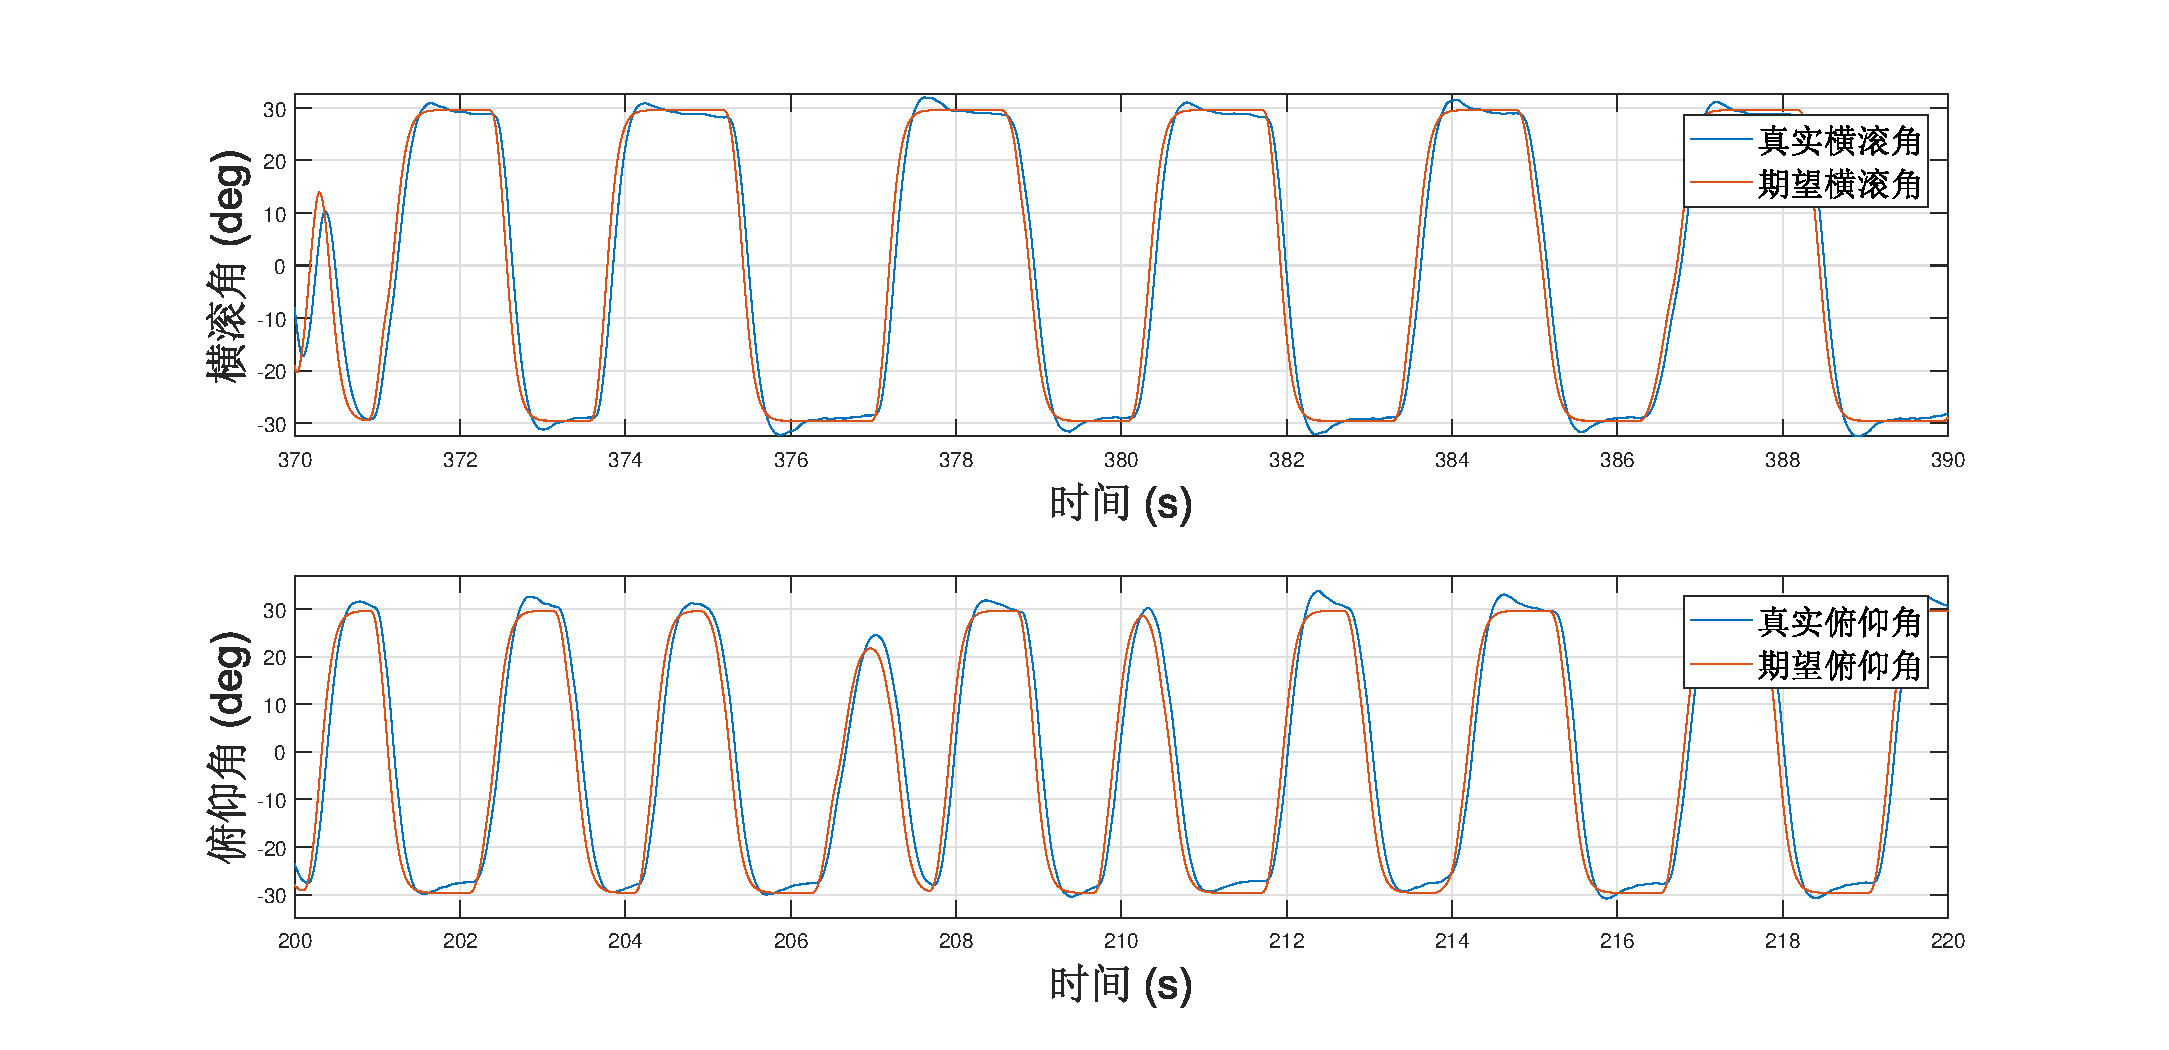
\includegraphics[width=1.0\textwidth]{rpcontrol.eps}
	\bicaption{横滚与俯仰跟踪结果}{Roll and pitch tracking results}
	\label{fig:Rptrackingresults}
\end{figure}

\begin{figure}[H]
	\centering
	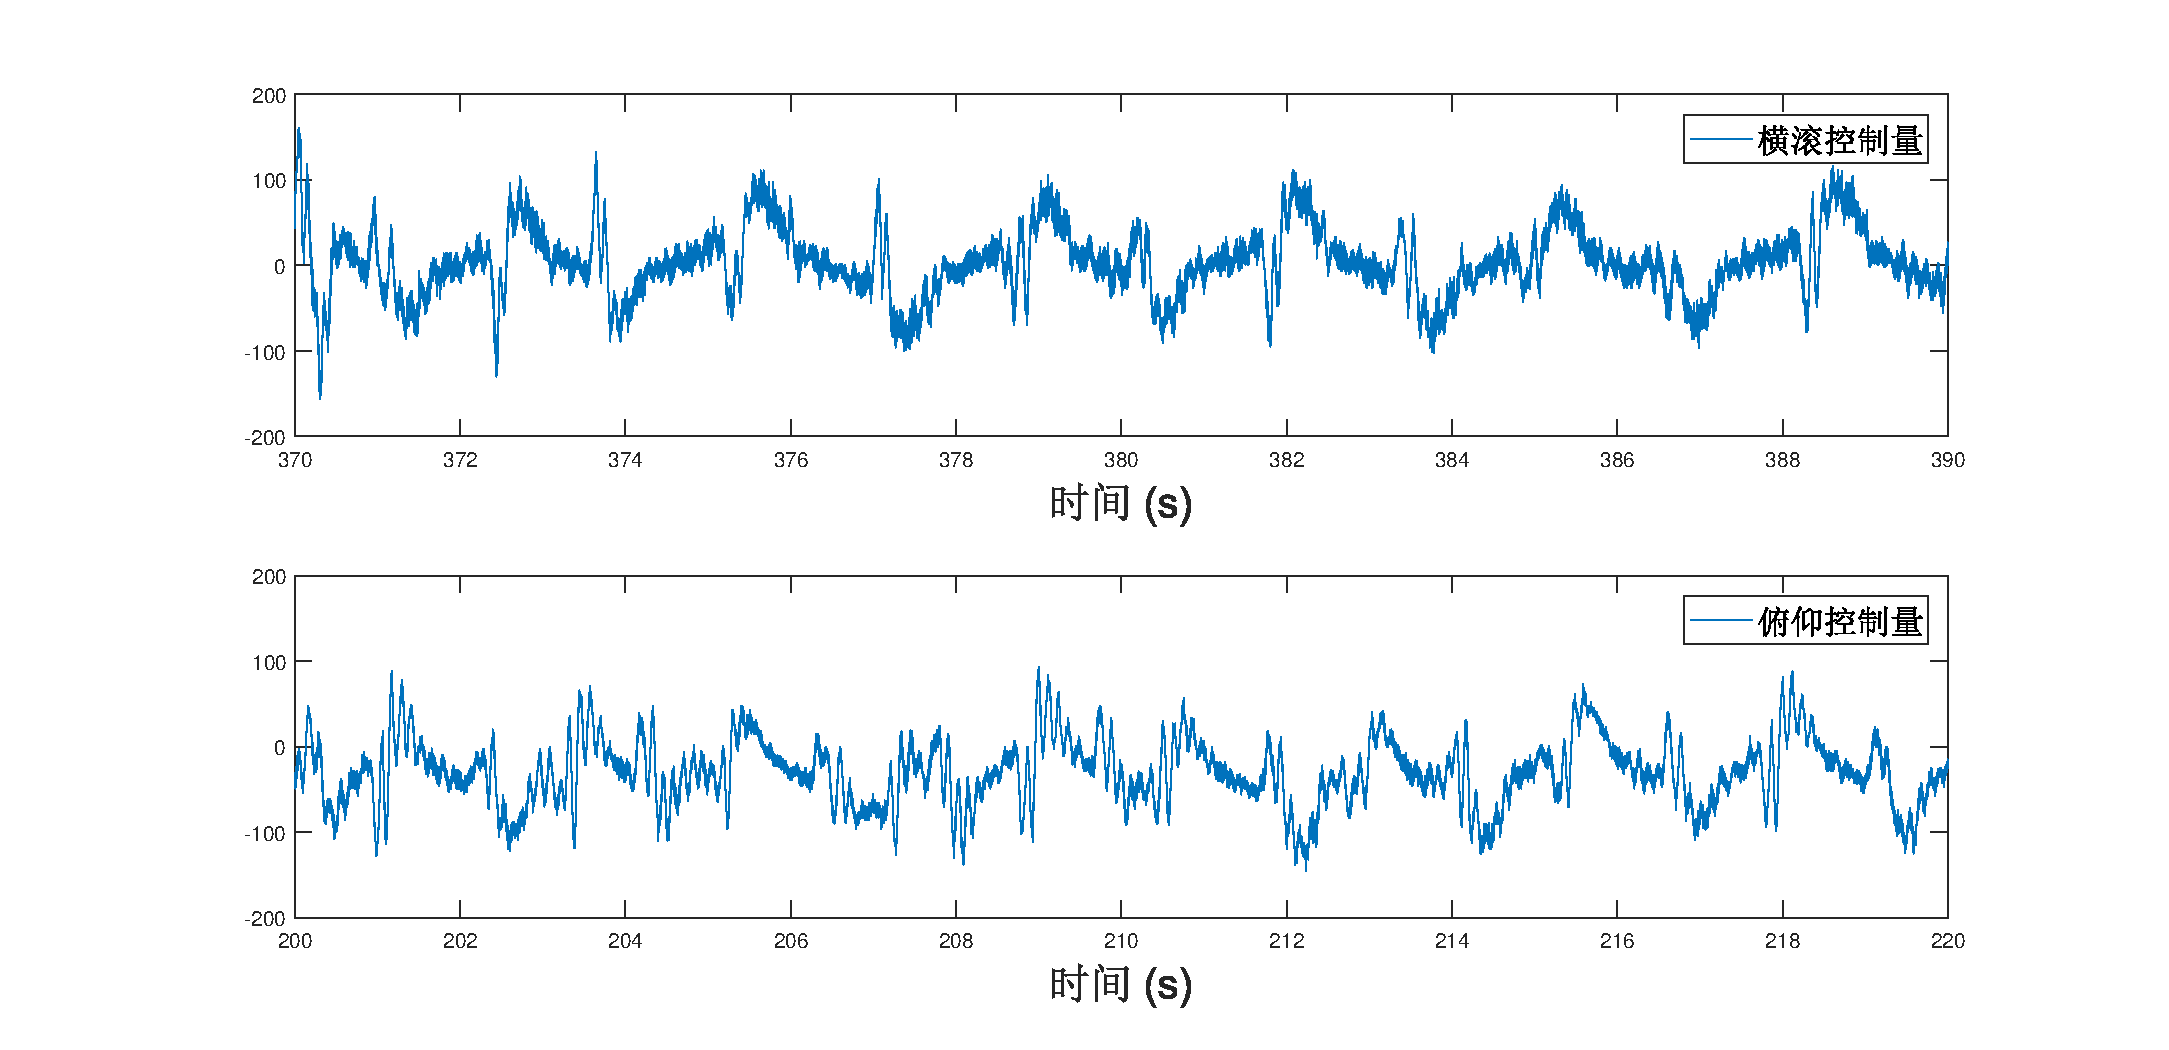
\includegraphics[width=1.0\textwidth]{u.eps}
	\bicaption{横滚与俯仰控制输出}{Roll and pitch control output}
	\label{fig:Rpcontroloutput}
\end{figure}

从\autoref{fig:Rptrackingresults}和\autoref{fig:Rpcontroloutput}可得出以下结论:

(1)姿态有一定的超调,但是超调后的回复过程是平稳的。

(2)观察控制俯仰角跟踪-30°期望角度时的结果可以看出,本文的算法存在一些稳态误差,后续可通过积分设计改善。

(3)整体控制输出较为平滑,可以满足实际飞行需求。

\gdutsubsection{位置控制实验}{Position control experiment}
本实验让飞行器定点悬停180s,记录机体位置的实际响应情况。
实验中设置飞行器期望位置$(x,y,z)$为(-1.60,-0.05,-0.47),设置期望速度为0,即定点悬停指令。
分别绘制定点悬停过程中飞行器的实际位置$x$和$y$如图\autoref{fig:xytrackingresults}所示,$z$方向和实际垂直速度变化情况如\autoref{fig:zdztrackingresults}所示。
%以下是测试结果。
%\begin{figure}[H]
%	\centering
%	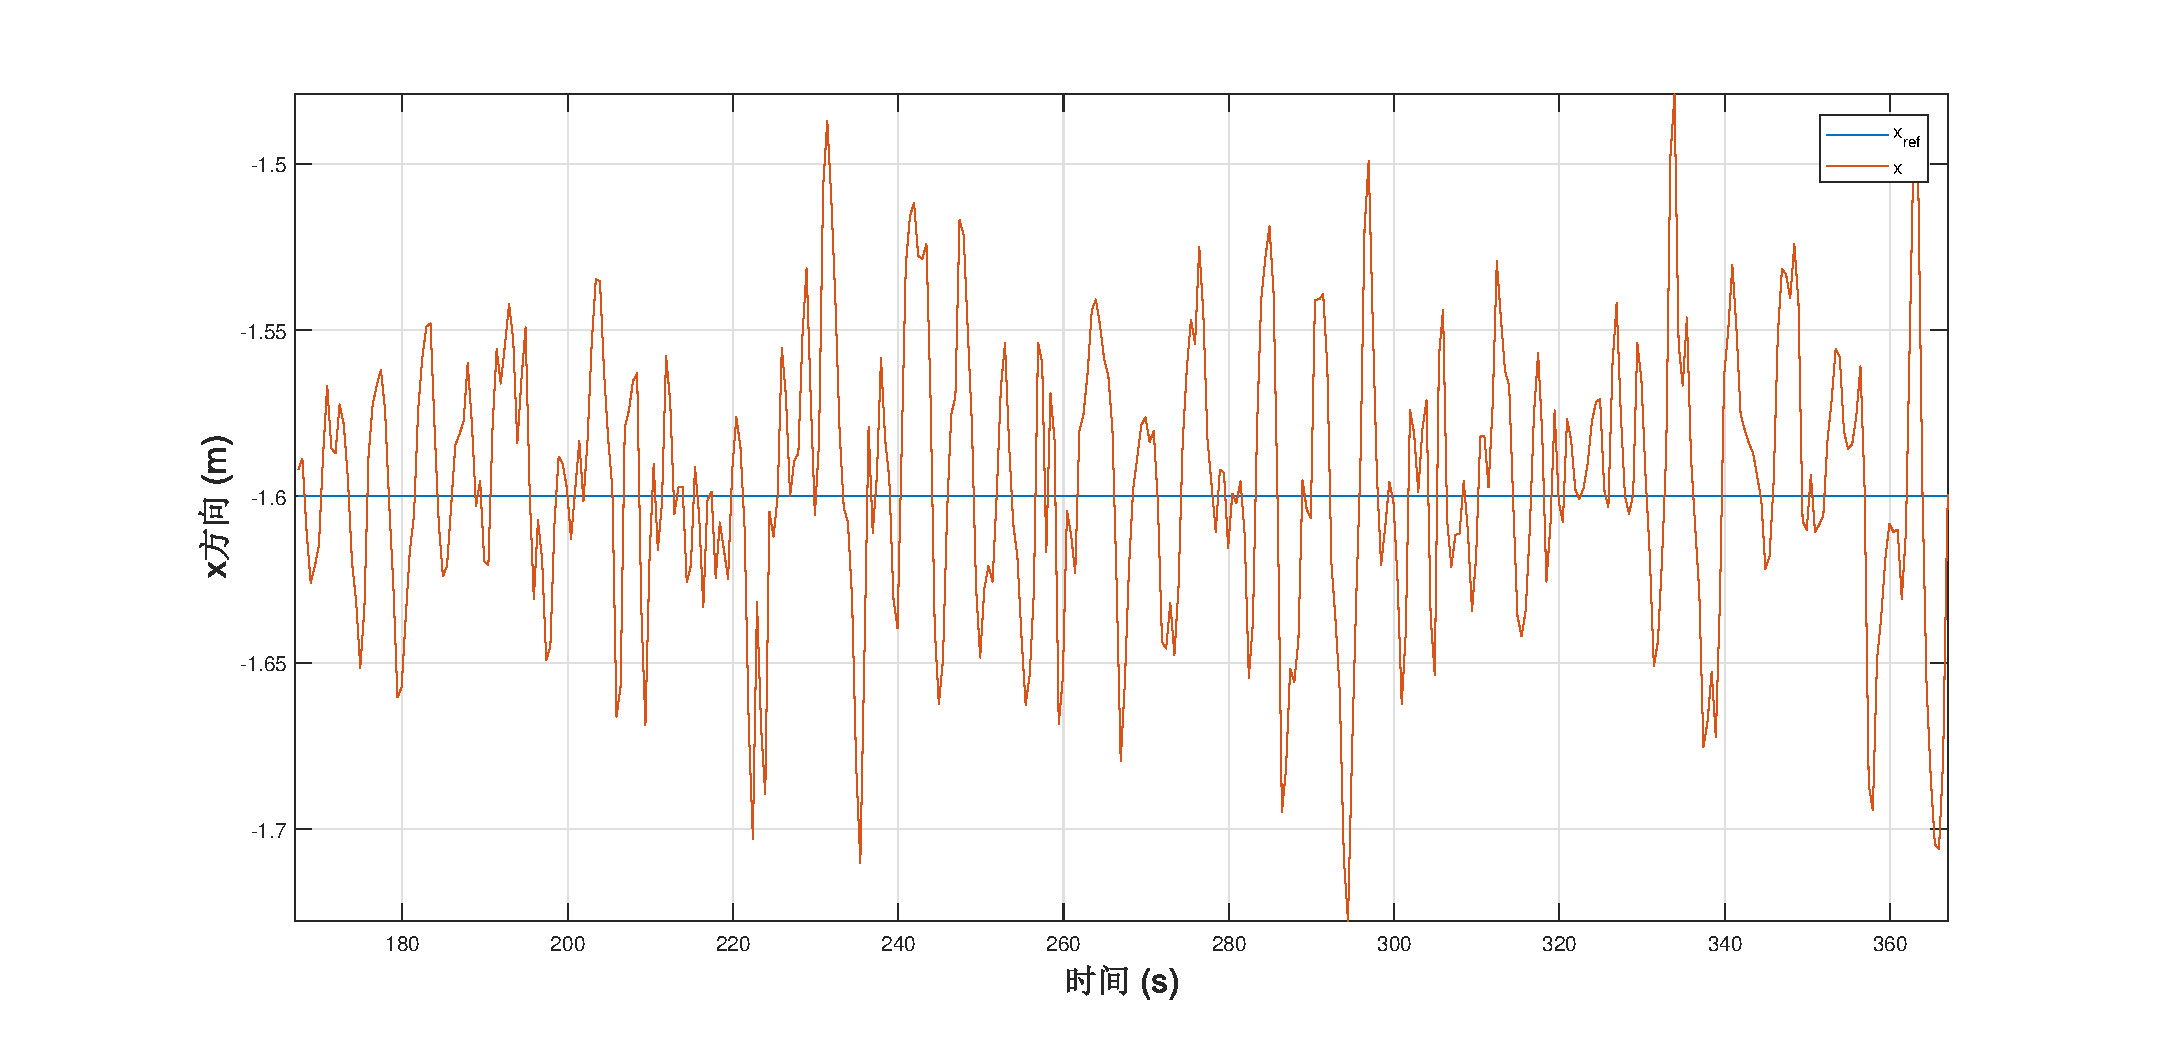
\includegraphics[width=1.00\textwidth]{xcontrol.eps}
%	\bicaption{x方向定位}{x tracking results}
%	\label{fig:xtrackingresults}
%\end{figure}
%
%\begin{figure}[H]
%	\centering
%	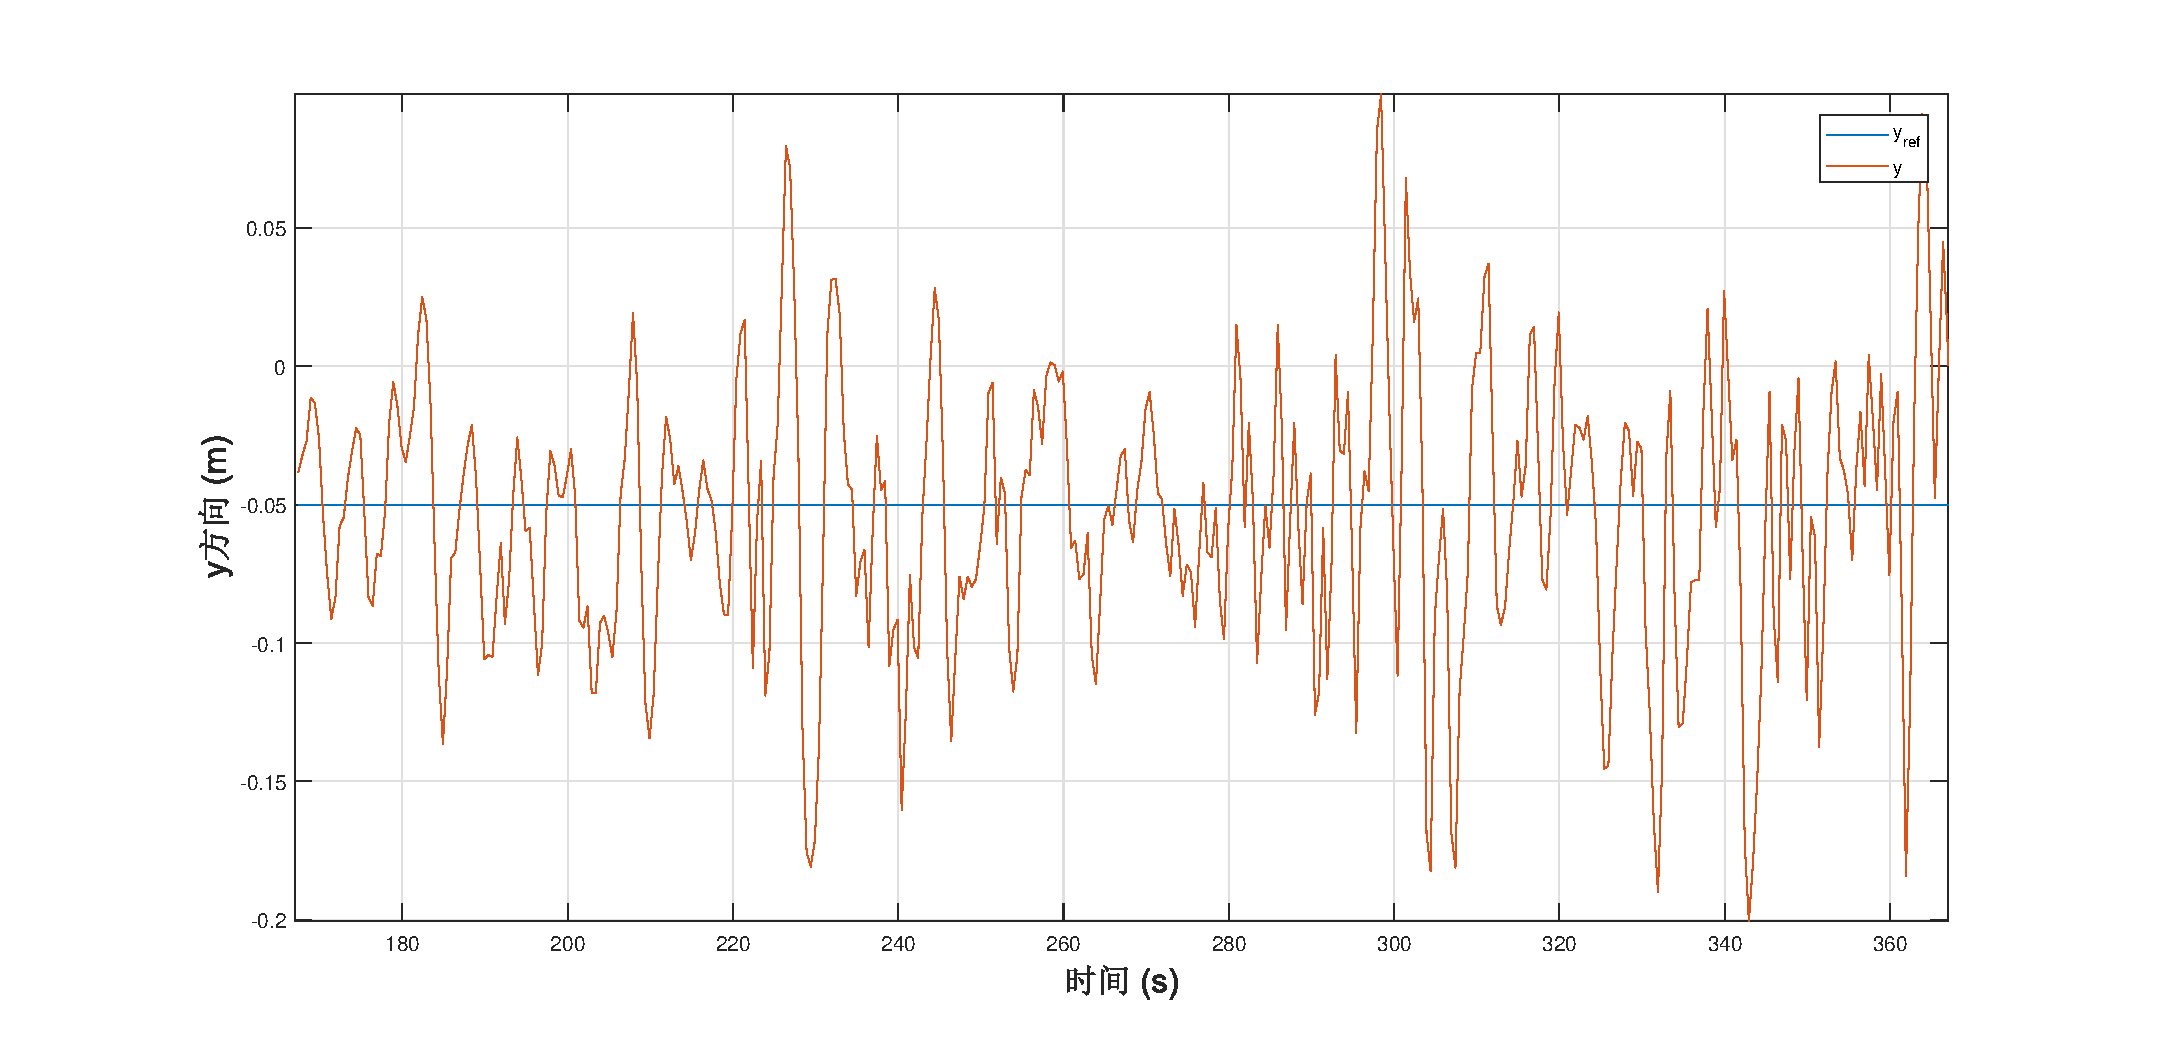
\includegraphics[width=1.00\textwidth]{ycontrol.eps}
%	\bicaption{y方向定位}{y tracking results}
%	\label{fig:ytrackingresults}
%\end{figure}
%
%\begin{figure}[H]
%	\centering
%	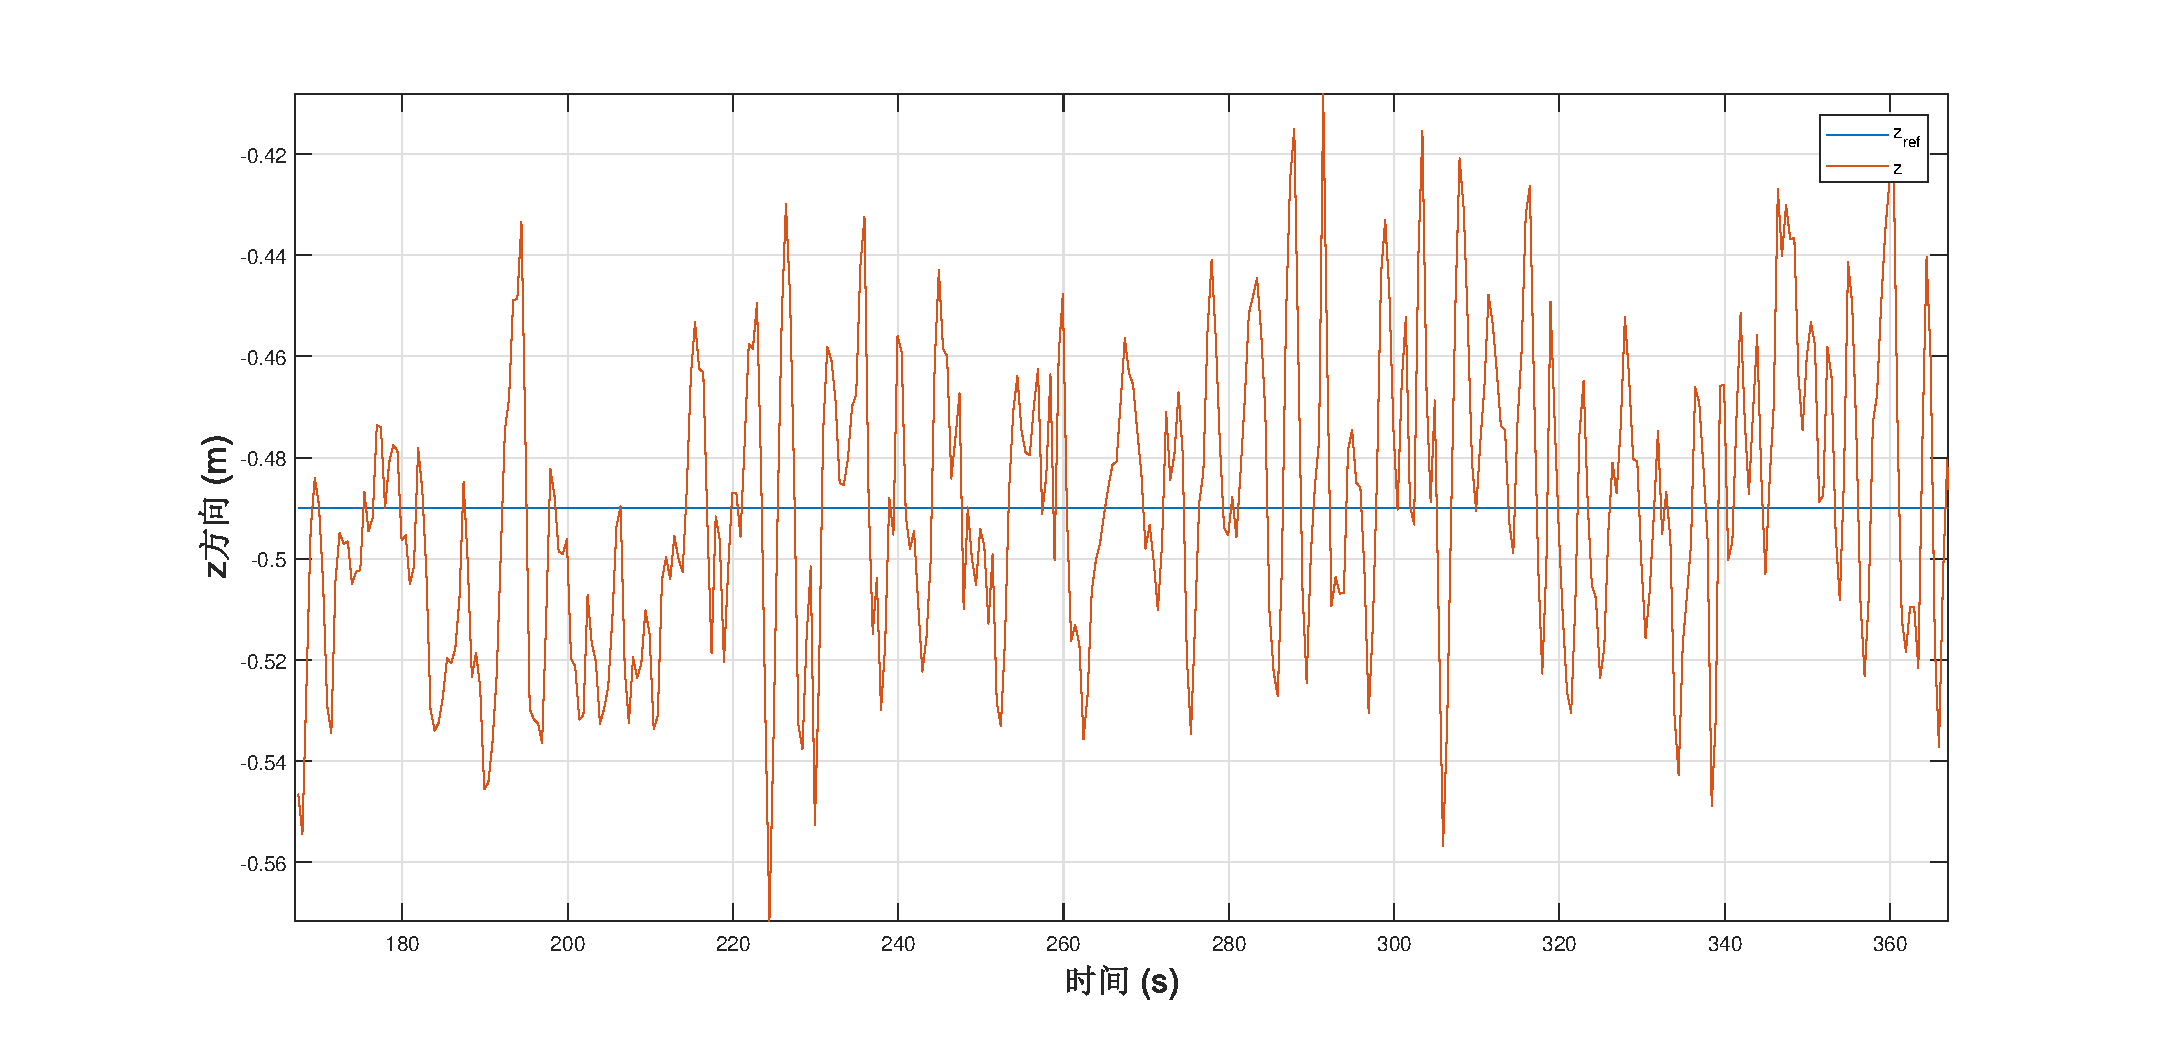
\includegraphics[width=1.00\textwidth]{zcontrol.eps}
%	\bicaption{z方向定位}{z tracking results}
%	\label{fig:ztrackingresults}
%\end{figure}
%
%\begin{figure}[H]
%	\centering
%	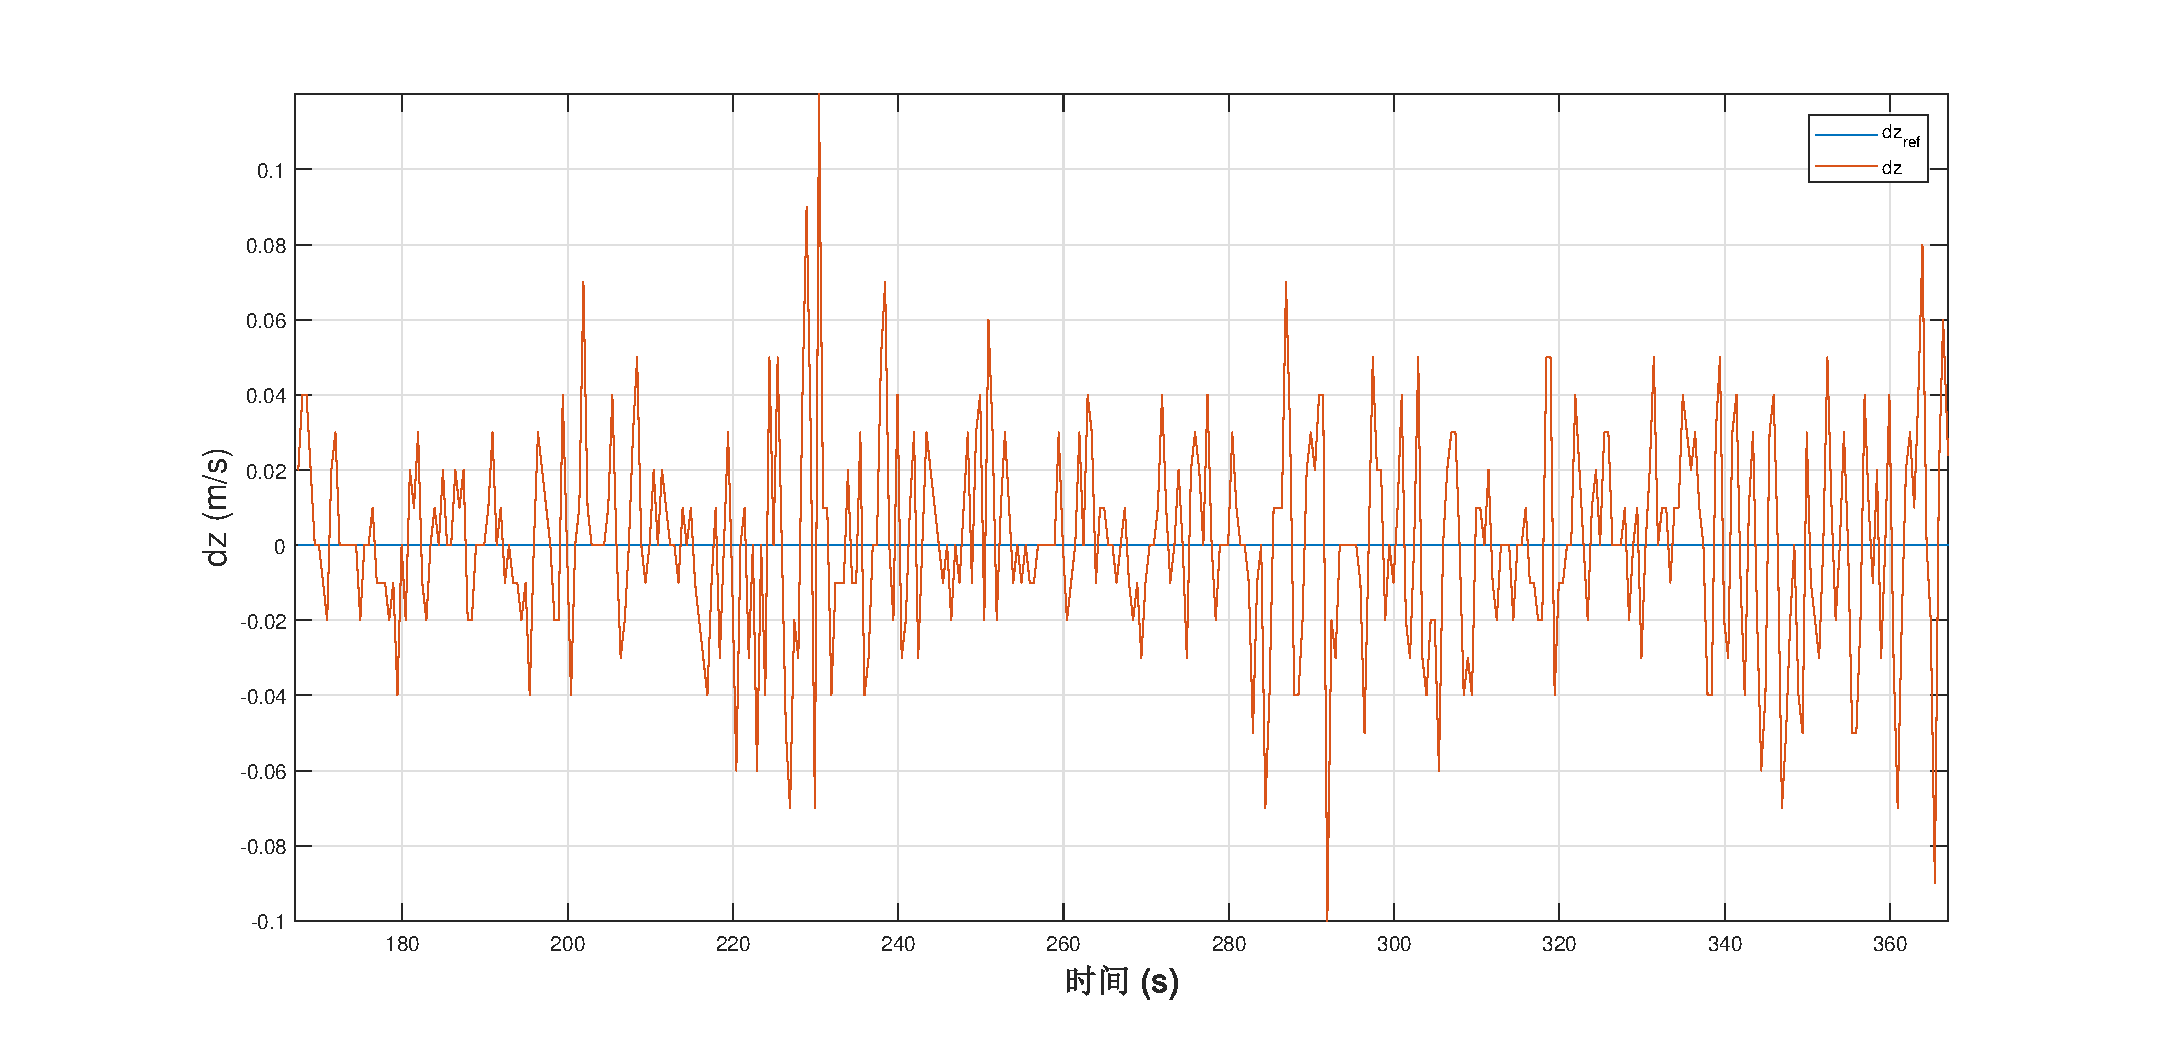
\includegraphics[width=1.00\textwidth]{dzcontrol.eps}
%	\bicaption{垂直速度保持情况}{Vertical velocity tracking results}
%	\label{fig:zveltrackingresults}
%\end{figure}

\begin{figure}[H]
	\centering
	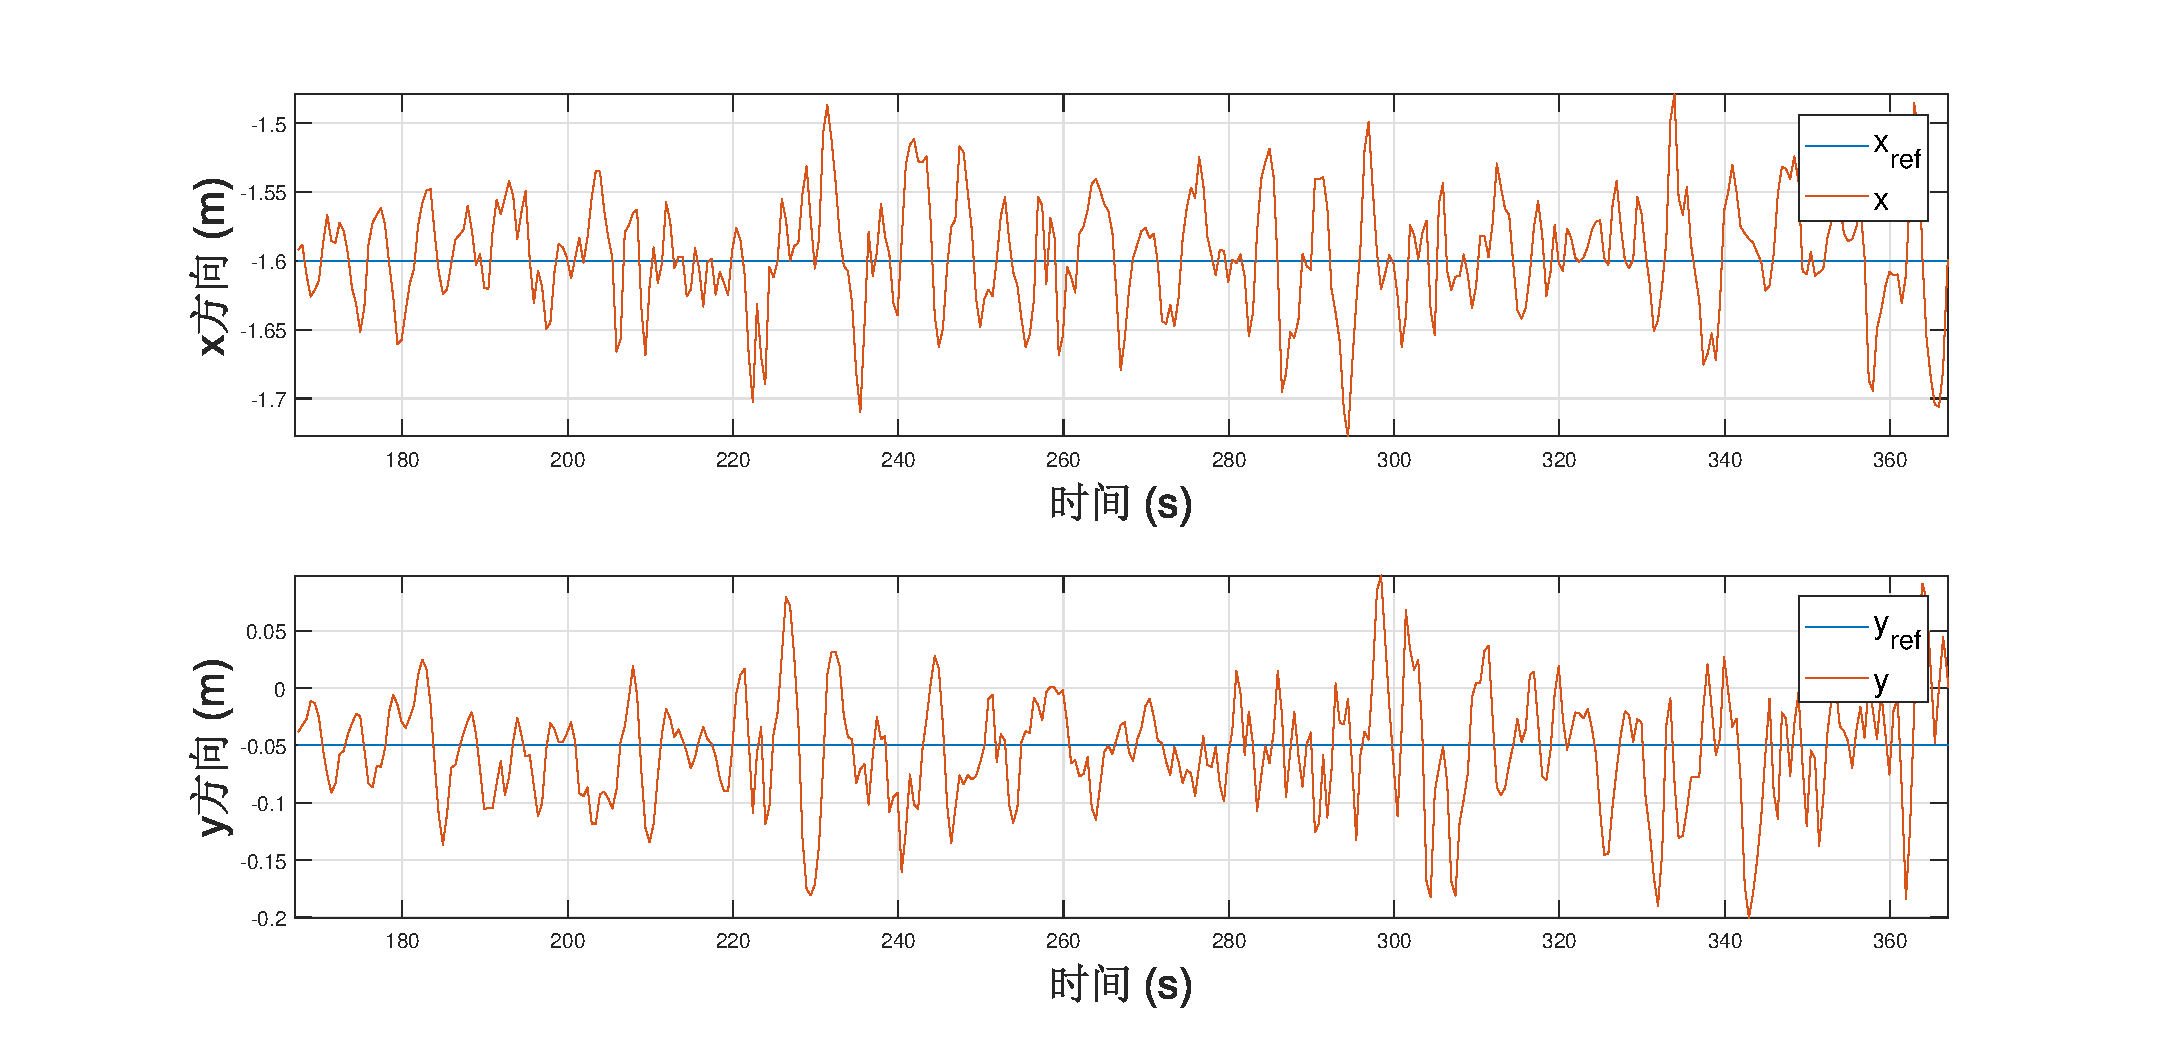
\includegraphics[width=1.00\textwidth]{xycontrol1.eps}
	\bicaption{xy方向定位}{xy tracking results}
	\label{fig:xytrackingresults}
\end{figure}

\begin{figure}[H]
	\centering
	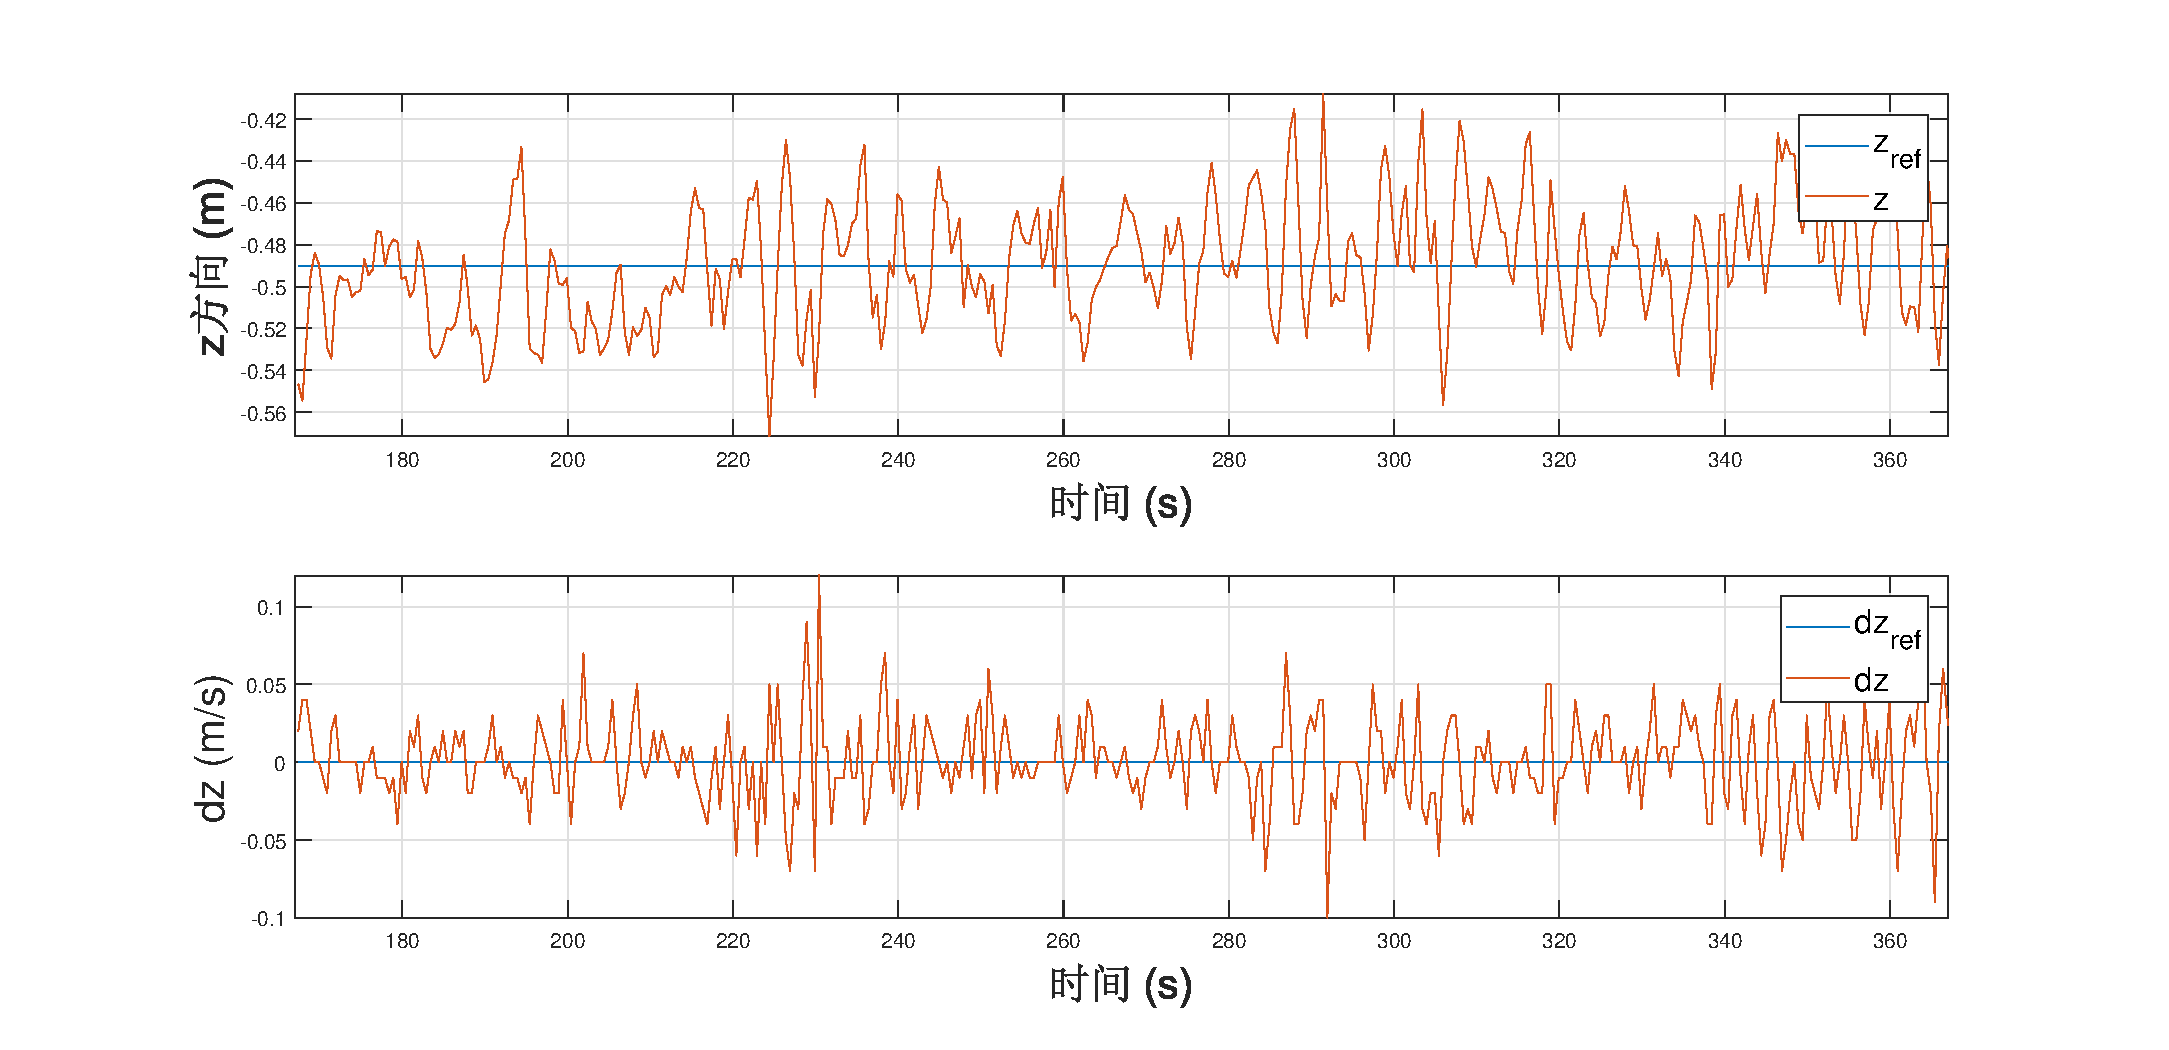
\includegraphics[width=1.00\textwidth]{zdzcontrol1.eps}
	\bicaption{z方向定位以及垂直速度保持情况}{z and dz tracking results}
	\label{fig:zdztrackingresults}
\end{figure}

从\autoref{fig:xytrackingresults}和\autoref{fig:zdztrackingresults}中定性分析当前位置是否能稳定工作在期望位置以评估位置控制器的性能。
显然,实验过程中飞行器的实际三维位置在期望三维位置的小范围内波动,表明当前位置是能收敛到期望位置。

最后,本实验通过采用实际位置平均值、实际位置误差均方差以及位置最大偏差三个指标来定量评估控制器的控制性能。
实际位置误差均方差是计算实际位置与期望位置的误差的均方差,位置最大误差是当前位置偏离期望位置的最大距离。
实际位置误差均方差和位置最大误差越小,控制性能越好。
具体指标计算结果如\autoref{Positiontrackingerror}所示。
\begin{table}[H]
	\bicaption{位置定位误差}{Position tracking error}
	\label{Positiontrackingerror}
	\begin{tabular}{ccccc}
		\toprule
		状态 & 给定位置($m$) & 实际位置平均值($m$) & 实际位置误差均方差($m$) & 位置最大偏差($m$)\\
		\midrule
		$x$ & -1.6000 & -1.6014 & 0.0600 & 0.1200 \\ 
		$y$ & -0.0500 & -0.0598 & 0.0732 & 0.1500 \\
		$z$ & -0.4700 & -0.4796 & 0.0320 & 0.0600 \\
		$dz$ & 0.0000 & 0.0075 & 0.0296 & 0.1000 \\
		\bottomrule 
	\end{tabular}
\end{table}

从\autoref{Positiontrackingerror}中可得出以下结论:

(1)由于位置传感器是使用GPS,GPS反馈的位置数据本身有比较明显的波动,这是抛开控制器性能差异外影响定位精度的重要因素。

(2)从$x$和$y$方向的位置波动程度来看,定位波动小于0.2m。抛开传感器信息反馈波动外,从控制器的角度上来看,定位效果满足飞行需求。

(3)从$z$方向和垂向速度的跟踪情况来看,高度波动小于0.2m,高度控制能满足飞行需求。

\gdutsection{总结与讨论}{Summary and discussion}
本章整合了现有的控制算法,完成了整个飞行控制系统的闭环,实现飞行器的稳定飞行,验证了本文提出的状态估计算法的有效性。
对于控制算法本身,还有很多工程细节可以处理,如使用扩展状态观测器获得更平滑的角速度,使用跟踪微分器生成前馈量等。
%由于时间有限,本文没有对更优的控制算法进行研究。

\gdutbackmatter
\gdutchapter{结论与展望}{Conclusion and prospect}
传感器的误差校准与多源信息融合技术对于提高多旋翼飞行器中状态估计精度与鲁棒性具有重要意义。
从提高低成本IMU测量精度和机载传感器抗干扰融合两方面技术问题出发,开展的研究工作包括:基于多位置法的IMU校准方法、基于多频率和多延时的传感器融合方法和传感器扰动抑制算法。
此外,在上述状态估计研究基础上,本文设计了控制算法,开发了一个完整的飞行控制系统,以进行飞行实验对提出的状态估计方法性能进行验证。

%本文展示了对飞行器自主飞行的最新技术的贡献,大部分贡献是状态估计算法。
%在第三章中,开发了状态估计算法,提出了一种模块化和可扩展的方法,该方法能够以一致的方式组合来自多个传感器的信息。
%在第四章中,开发了传感器校准算法,能够在没有外部设备的情况下对传感器进行高精度的校准。
%在第五章中,开发了控制算法并结合前两章的算法形成一个集成的飞行器系统。
%
%本文注意到,虽然本文的实验平台是多旋翼飞行器,但本文的方法不限于这一特定类型的平台。
%实际上,本文的方法是基于传感器的,同样适用于其他机器人,如固定翼、地面机器人等。
\gdutbacksection{成果总结}
综上所述,本文的主要贡献如下:
\begin{itemize}
	\item 针对IMU校准精度不足的问题,提出了一种检测阈值最优计算算法,解决了阈值计算非最优造成的校准结果精度不足的问题。
	\item 针对多源信息融合问题,提出了预测-修正-延时融合框架,在不需要调整算法的情况下可添加或减少传感器,解决了多源信息融合的问题。
	\item 针对传感器扰动问题,提出了偏航角解耦策略以及运动加速度插值延时补偿算法,解决了因运动加速度或磁场干扰影响飞行稳定性的问题。
	\item 设计了控制算法,完成了飞行控制系统的闭环,并通过实验表明,飞行控制系统是稳定可靠的。
\end{itemize}

\gdutbacksection{未来研究展望}
本文涉及到了几个有趣的研究领域,其中一些是随着飞行器技术的发展而不断发展成大型系统的,而另一些则是在评估最新方法的性能时值得追求的新方向。
\paragraph{自主飞行中估计与控制的耦合设计。}
在本文目前的工作中,控制器与估计器是分开设计的。然而,随着飞行器朝着高速自主飞行的方向发展,可能会要求估计器和控制器耦合设计,以生成和执行高效、无碰撞和安全的飞行轨迹。
\paragraph{用于飞行器的新的传感器技术。}
虽然传统的传感器如IMU、GPS、相机已被证明可用于飞行器导航,但最近传感技术的发展可能创造新的机会。例如,光场可以作为深度感知的传感器。这些新型传感技术在飞行器上的应用具有很大的潜力。
\paragraph{传感器和能观性研究。}
众所周知,传感器数量越多,系统的能观性越好,但单个传感器对系统能观性的影响尚不清楚。增加更多的传感器会带来出更多的能观性,但是传感器提供的信息以及信息的质量会导致能观性的复杂判断条件。因此,一个能够以在线方式识别能观性的通用框架将有利于更高层次的任务,如运动规划和风险评估。

\nocite{*}% 列出全部参考文献
\printbibliography

\gdutchapter{攻读学位期间取得与学位论文相关的成果}{Publication and patents during study}

\gdutbacksection{申请发明专利}

\begin{results}
  \item 鲁仁全, \textbf{邓正雄}, 徐雍, 林明, 饶红霞. 全方位移动侦查探测器、控制系统和控制方法. 发明专利申请号: 202011588192.4.
%  \item ***, \textbf{2111904069}, ***, ***, ***. 全方位移动侦查探测器、控制系统和控制方法. 发明专利申请号: 202011588192.4.
\end{results}

\gdutstatement

\gdutchapter{致谢}{Acknowlegements}
没有大家的支持,这篇论文是不可能完成的。
首先,我要感谢我的导师鲁仁全教授和徐雍教授,感谢他们在我在广工的研究生学习过程中给予我的支持和指导。
此外,我要感谢智能决策与协同控制研究所的同学和老师,以及海雀团队的师兄师弟们。
我们三年来进行了许多很棒的技术讨论和有趣的时光。
还有,我要感谢柯金铭、邝野和滕达,感谢他们三年来对我生活上和学习上的帮助。
特别地,我要感谢刘畅、邓华银、陈梓杰和凌胜财,感谢他们对我在撰写毕业论文上的帮助。
我感谢我的父母,感谢多年来他们给予我的爱和支持。

%没有大家的支持,这篇论文是不可能完成的。
%首先,我要感谢我的导师***和***,感谢他们在我在广工的研究生学习过程中给予我的支持和指导。
%此外,我要感谢智能决策与协同控制研究所的同学和老师,以及海雀团队的师兄师弟们。
%我们三年来进行了许多很棒的技术讨论和有趣的时光。
%还有,我要感谢***、***和***,感谢他们三年来对我生活上和学习上的帮助。
%特别地,我要感谢***、***、***和***,感谢他们对我在撰写毕业论文上的帮助。
%我感谢我的父母,感谢多年来他们给予我的爱和支持。
%\gdutappendix
%
%\gdutchapter{附录标题}{The appendix title}
%对需要收录于学位论文中且又不适合书写于正文中的附加数据、资料、详细
%公式推导、计算机程序等有特色的内容,可做为附录排写。
\end{document}